% ================================================================== %
\documentclass{article}
\usepackage{mathsnotes}

% Course Details
\course{Coding and Cryptography}
\term{Lent 2024--25}
\lecturer{Rachel Camina}
\tripospart{Part II of the Mathematical Tripos}
\university{University of Cambridge}
\name{Avish Kumar}
\email{ak2461@cam.ac.uk}
\website{https://ak1089.github.io/maths/notes}
\version{1.23}
\disclaimer{These notes are unofficial and may contain errors. While they are written and published with permission, they are not endorsed by the lecturer or University.}

% Auxiliary files
\input{../graphs.tikzstyles}

% Format the document
\begin{document}
\makecover
% ================================================================== %

\section{Noiseless Coding}
\subsection{The Coding Problem}
\label{section-noiseless-coding-problem}

The general problem of coding is that of
transmitting a message across a communication channel.
For example, if we wish to send an email containing a message $m =$ ``Call me!",
we may encode this as a sequence of binary strings using the standard ASCII format.

Under this code, $f(``C") =$ \texttt{1000011}.
In fact, each character is mapped to seven binary digits, or \textit{bits}.
The entire message is the concatenation of these strings: ``Call me!" becomes:
\[
f^*(\text{``Call me!"}) = 
\texttt{10000111100001110110011011000100000110110111001010100001}.
\]

\begin{definition}[Source, Encoder, Channel, Receiver, Decoder]
    \label{source-encoder-channel-receiver-decoder}
    More generally, we have a \textit{source}, often called Alice.
    She uses an \textit{encoder} to convert plaintext messages into encoded messages.
    These encoded messages are sent through a \textit{channel}:
    this channel may be \textit{noisy}, and introduce errors into the code.
    The encoded message is received by a \textit{receiver} Bob,
    who uses a \textit{decoder} to convert it back into the original plaintext.
\end{definition}

Given a source and a channel, described probabilistically, we want to design an encoder and decoder in order to transmit source information across the channel. We might want certain properties:

\begin{enumerate}
    \item Economy: we would like to minimise the amount of unnecessary information sent: the code should not be too long, as it wastes time and money.
    \item Reliability: the decoder should be able to successfully decipher the plaintext with very high probability, or mistakes should be detectable.
    \item Privacy: we may want only someone with the decoder to be able to read the message.
\end{enumerate}

Accomplishing this last desideratum is the aim of \textit{cryptography} in particular, while \textit{coding} deals with the first two. How might we achieve these?

\begin{remark}[Economy and Reliability]
	\label{economy-and-reliability}
    Morse code is \textit{economic} in that it attempts to minimise message length.
    This is done by giving shorter codes to letters which are used more frequently:
    $E = \cdot$, while $Q = -- \cdot --$.

	The ISBN system for numbering books is \textit{reliable}. Each book has a unique ten-digit ISBN: the first nine digits encode information about the book (its publisher, ID, and region) while the last digit is a \textit{check digit} chosen such that $10 a_1 + 9 a_2 + \dots + 2a_9 + a_{10} \equiv 0 \pmod{11}$.
	
	This has robust error-detection capabilities. For example, a transposition of any two digits $a_{i}$ and $a_{j}$ will add $(j-i)(a_{j} - a_i) \not\equiv 0 \pmod{11}$ to the left hand side. This means a single error can be detected, since the congruence will be broken.
\end{remark}

% ================================================================== %

\subsection{Communication Channels}
\label{section-noiseless-communication-channels}
\vskip 8pt

\begin{definition}[Channel]
	\label{channel-definition}
    A \textit{communication channel} takes letters from an input alphabet
    $\Sigma_1 = \set{a_1, \dots, a_r}$
    and emits letters from an output alphabet
    $\Sigma_2 = \set{b_1, \dots, b_s}$.
    It is determined by the probabilities
	\[
	\P[y_1\dots y_k \text{ emitted} \mid x_1\dots x_k \text{ input}]
	\where x_i \in \Sigma_1^*, y_i \in \Sigma_2^*.
	\]
\end{definition}

\begin{note}
	The important feature of a channel is that it is not necessarily perfect!
	Much like in the real world,
	where we deal with problems like TV static or data corruption,
	the channels we will study are affected by noise.
\end{note}

\begin{definition}[Discrete Memoryless Channel]
	\label{discrete-memoryless-channel}
    A \textit{discrete memoryless channel} over a finite alphabet
    is a channel for which the probabilities
	\[
	P_{ij} = \P[b_j \text{ received} \mid a_i \text{ sent}]
	\]
	are the same every time the channel is used,
	independent of past and future channel use.
	This is the \textit{memoryless property},
	while the discrete nature is given by the alphabets.
\end{definition}

We often identify the channel with its \textit{channel matrix} $P$,
which is the $r \times s$ matrix
with entries $p_{ij}$ equal to those probabilities.
Note that the rows of $P$, but not necessarily its columns, sum to 1,
and all entries are non-negative:
we thus say that $P$ is a \textit{stochastic matrix}.

\begin{example}[Binary Symmetric/Erasure Channel]
	\label{binary-symmetric-erasure-channel}
	For example, a Binary Symmetric Channel
	with probability $0 \leq p \leq 1$ of error
	is a DMC over the binary alphabet $\Sigma_1 = \Sigma_2 = \binset$.
	In particular, any bit sent has a probability $p$
	of being flipped by the channel due to noise.
	This can be seen in the below diagram.

	\ \ctikzfig{binary-symmetric-channel-definition} \

	Usually, we assume $p < 0.5$.
	If $p > 0.5$,
	then we can just pre-flip the bits sent to reduce the error probability
	(since any bit is likely flipped back by the channel).
	If $p = 0.5$,
	then every single bit received is equally likely to be \texttt{0} and \texttt{1},
	independently of what was actually transmitted,
	so the channel is entirely useless (pure noise).

	A Binary Erasure Channel is similar,
	taking $\Sigma_1 = \binset$ but
	$\Sigma_2 = \set{\texttt{0}, \texttt{1}, \texttt{*}}$,
	with the \texttt{*} understood to be an \textit{erasure}.
	Each bit transmitted has a probability $0 \leq p \leq 1$ of being erased,
	making it unreadable,
	and is transmitted correctly otherwise (never flipped), giving:

	\ \ctikzfig{binary-erasure-channel-definition} \

	where the columns correspond to \texttt{0}, \texttt{*}, and then \texttt{1}.
\end{example}

\begin{definition}[Capacity]
	\label{capacity-definition-heuristic}
    The \textit{capacity} of a channel is
    the highest rate at which information
    can be reliably transmitted over the channel.
    Here, the rate is measured as units of information per unit time:
    for a binary channel, this might be
    the number of decoded bits per transmitted bit.
    High reliability is achieved by
    an arbitrarily low probability of error.
\end{definition}

% ================================================================== %

\subsection{Strings and Alphabets}
\label{section-noiseless-strings-and-alphabets}

We frequently work with alphabets,
which are simply sets of elements called letters or characters.
These are the building blocks of a language:
the input alphabet of a code is the set of atoms
which are encoded into something else.

\begin{definition}[String, Concatenation, Length]
	\label{string-concatenation-length}
	For an alphabet $\Sigma$,
	we define the set of $\Sigma$-strings to be
	$\Sigma^* = \bigcup_{n \geq 0} \Sigma^n$.
	These are usually written as concatenations rather than tuples,
	so that the set of binary alphabet strings is
	\[
	\Sigma_\texttt{01}^* = \set{
	\eps, \texttt{0}, \texttt{1},
	\texttt{00}, \texttt{01}, \texttt{10}, \texttt{11},
	\texttt{000}, \texttt{001}, \texttt{010}, \texttt{011},
	\texttt{100}, \texttt{101}, \texttt{110}, \texttt{111},
	\texttt{0000}, \texttt{0001}, \dots }
	\]
	The \textit{length} of a string
	is the number of letters contained.
	Here $\eps$ is the empty string with length 0.
	If $x = x_1x_2\dots x_r$ and $y = y_1 y_2\dots y_s$ are $\Sigma$-strings,
	their \textit{concatenation} is given by $xy=x_1 \dots x_r y_1 \dots y_s$.
\end{definition}

For two alphabets $\Sigma_1$ and $\Sigma_2$, a \textit{code} is a function $f: \Sigma_1 \to \Sigma_2^*$. The strings $\set{f(x): x \in \Sigma_1}$, or the image of $f$, are called codewords.

\begin{example}[Polybius Square]
	\label{polybius-square-example}
    For example, the Polybius Square
    is a cipher developed by Ancient Greek polymath Polybius,
    who created a way to encode Greek as numbers.
    
    The input alphabet $\Sigma_1$
    was the 24 Greek letters $\alpha$ to $\omega$,
    while the output alphabet $\Sigma_2$
    was the set $\set{1, 2, 3, 4, 5}$.
    Each letter was mapped to precisely two digits from 1 to 5
    for easy transmission (using every pair except 55).
    This made the codewords the set
    \[
	\set{1 \dots 5}^2 =
	\set{11, 12, 13, 14, 15, 21, 22, \dots 52, 53, 54}.
	\]
\end{example}

\begin{note}
	 For English-language codes,
	 we do not necessarily have $\Sigma_1$ being
	 $\set{\mathrm{a} \dots \mathrm{z}}$
	 the set of letters.
	 The domain of the code function is the set of atoms of the code,
	 which is often pairs of letters, or even more commonly entire words.
\end{note}

We apply a code by encoding
$x_1x_2\dots x_n \in \Sigma_1^*$ as
$f(x_1)f(x_2)\dots f(x_n) \in \Sigma_2^*$.
This extends $f$ the code function
from atoms to entire words in the input language,
which we call $f^*: \Sigma_1^* \to \Sigma_2^*$.

However, not every function $f: \Sigma_1 \to \Sigma_2^*$ works as a code.

\begin{definition}[Decipherable]
	\label{decipherable-definition}
    A code $f$ is \textit{decipherable} if $f^*$ is injective,
    so that every string in $\Sigma_2^*$ arises from at most one message.
    Without this condition, the output of encoding
    might have come from multiple possible inputs,
    and we would have no way of knowing which when decoding it.
\end{definition}

\begin{proposition}[Decipherability requires injectivity]
	\label{decipherability-requires-injectivity}
	A decipherable code $f$ requires $f$ injective.
	However, this is not a sufficient condition.
\end{proposition}

\begin{prf}
    Firstly, if $f$ is not injective,
    then $f(x) = f(y)$ where $x \neq y \in \Sigma_1$.
    But then the encoding of $x$ and $y$
    when treated as members of $\Sigma_1^*$ is the same,
    violating injectivity of $f^*$.
    
    However, this is not a sufficient condition.
    Suppose $\Sigma_1 = \set{1, 2, 3, 4}$ and $\Sigma_2 = \binset$.
    Define
    \[
	f(1) = \texttt{0}
	\qquad
	f(2) = \texttt{1}
	\qquad
	f(3) = \texttt{00}
	\qquad
	f(4) = \texttt{01}
	\]
	so that $f$ is injective,
	but $f^*(1112) = \texttt{0001} = f^*(34)$,
	so $f^*$ is not.
\end{prf}

How do we construct decipherable codes?
There are a few basic properties of codes which guarantee decipherability
(none of these are necessary, but are all sufficient)
provided that $f$ is injective.

\begin{enumerate}
    \item A \textit{block code} is a code where all codewords are of the same length. For example, the Polybius cipher had all codewords of length 2, and so it can be decoded by considering the output as a list of length-2 strings.
    \item A \textit{comma code} reserves one letter in $\Sigma_2$ to act as the comma, which appears at the end of every output of $f$ and nowhere else. It thus delimits words in $\Sigma_2^*$, so we know where each letter in the original input to the code was mapped.
    \item A \textit{prefix-free} (or \textit{instantaneous}) code is a code where no codeword is a prefix of any other codeword: for any $x, y \in \Sigma_1$, we have $f(x) \neq f(y)\alpha$ for any $\alpha \neq \eps \in \Sigma_2^*$.
\end{enumerate}

\begin{note}
	In fact, block codes and comma codes are special cases of prefix-free codes.
\end{note}

\begin{theorem}[Kraft's Inequality]
	\label{krafts-inequality}
    Let $\Sigma_1 = \set{x_1, \dots x_m}$
    and $\abs{\Sigma_2} = a$.
    Then a prefix-free code $f: \Sigma_1 \to \Sigma_2^*$
    with word lengths $s_1, \, \dots, \, s_m$
    (where $\abs{f(x_i)} = s_i$)
    exists if and only if
    \[
	\sum_{i=1}^m a^{-s_i} \leq 1
	\]
\end{theorem}

\begin{prf}
    ($\Rightarrow$)
    Consider an infinite tree
    where each node has $a$ descendents
    corresponding to the $a$ letters of $\Sigma_2$.
    Then each codeword corresponds to precisely one of these nodes,
    where the path to the node spells out the codeword along the branches taken.
    
    Assuming $f$ is prefix-free,
    no codeword is the ancestor of any other.
    View the tree as a network, with water being pumped in at the root,
    where each node divides the flow equally between each descendant.
    The total amount of water extracted at the codewords is therefore
    the sum of $a^{-s_i}$,
    which is at most the total amount of water pumped in,
    demonstrating the inequality. 
    
    \ \ctikzfig{kraft-inequality-tree-proof}
    
    ($\Leftarrow$)
    Conversely, we can construct a prefix-free code
    with word lengths $s_1 < s_2 < \cdots < s_m$.
    Choose codewords sequentially,
    ensuring that any previous codewords are not prefixes.
    Suppose that the $r\th$ codeword has no valid code available.
    Then constructing the tree above gives
    \[
	\sum_{i=1}^{r-1} a^{-s_i} = 1
	\implies
	\sum_{i=1}^{m} a^{-s_i} > 1
	\]
	which contradicts our assumption.
\end{prf}

\begin{theorem}[McMillan / Karush]
	\label{mcmillan-karush}
    Every decipherable code satisfies Kraft's inequality.
\end{theorem}

\begin{prf}
	Let $f: \Sigma_1 \to \Sigma_2^*$
	be a decipherable code with word lengths $s_1 \dots s_m$,
	where $s = \max s_i$.
	For any $r \in \N$, we must have
	\[
	\left( \sum_{i=1}^m a^{-s_i} \right)^r =
	\left( \sum_{\ell=1}^{rs} b_\ell a^{-\ell} \right)
	\]
	where $b_\ell$ is the number of ways
	of choosing $r$ codewords with total length $\ell$.
	Since $f$ is decipherable,
	we know that $b_\ell \leq \abs{\Sigma_2}^\ell = a^\ell$,
	since no string can be the encoding of more than one set of codewords.
	This means that we can write
	\[
	\left( \sum_{i=1}^m a^{-s_i} \right)^r \leq
	\left( \sum_{\ell=1}^{rs} a^\ell a^{-\ell} \right) =
	rs
	\implies
	\left( \sum_{i=1}^m a^{-s_i} \right) \leq
	(rs)^{1/r}
	\]
	But this is true for any $r$,
	and $(rs)^{1/r} \to 1$ as $r \to \infty$.
	Therefore the left hand side of the inequality is at most 1,
	which is exactly the statement of Kraft's inequality.
\end{prf}

As a result, we mostly restrict our attention to prefix-free codes.

% ================================================================== %

\subsection{Mathematical Entropy}
\label{section-noiseless-entropy}

Entropy is a measure of ``randomness" or ``uncertainty".
Suppose a random variable $X$
takes values $x_1 \dots x_n$
with probabilities $p_1 \dots p_n$,
where we have $0 \leq p_i \leq 1$ for all $i$
and $\sum p_i = 1$.
Loosely, the \textit{entropy} $H(X)$ is
the expected number of yes/no questions required to determine the value of $X$.

This is not a formal definition yet: we consider some examples first.

\begin{example}[Basic Entropy Examples]
	Let's consider $X$ taking values $x_1 \dots x_4$.
    
    If $p_1 = p_2 = p_3 = p_4 = 1/4$,
    then asking precisely two yes/no questions
    can consistently determine the value of $X$.
    For example, the two questions could be
    ``is $X \in \set{x_1, x_2}$?"
    and
    ``is $X \in \set{x_1, x_3}$?".
    Here, this means $H(X) = 2$ directly.
    
    Now, suppose
    $(p_1, p_2, p_3, p_4) = (1/2, 1/4, 1/8, 1/8)$.
    Then we could ask the question ``$X = x_1?$"
    and finish with one question half the time.
    If the answer is no, we ask ``$X = x_2?$"
    and again be done half the time (so a quarter overall).
    Failing that, we ask ``$X = x_3?$"
    and know the value of $X$ with certainty after three questions.
    
    This gives
    $H(X) = 1 \times 1/2 + 2 \times 1/4 + 3 \times 1/8 +  3 \times 1/8 = 7/4 < 2$,
    and so the first random variable is ``more random".
    This aligns with our intuition.
\end{example}

This gives us enough to write down our formal definition.

\begin{definition}[Entropy]
	\label{random-variable-entropy}
    For a random variable $X$
    taking values $x_1 \dots x_n$
    with probabilities $p_1 \dots p_n$,
    where we have $0 \leq p_i \leq 1$ for all $i$
    and $\sum p_i = 1$,
    the \textit{entropy} $H(X)$ is defined to be
    \[
	H(X) = H(p_1, \dots, p_n) =
	-\sum_{i=1}^n p_i \log p_i.
	\]
\end{definition}

\begin{note}
	In this course, we always consider the logarithm to be defined as $\log_2$
	(the logarithm with base 2),
	rather than the natural logarithm with base $e$,
	due to our focus on binary.
\end{note}

\begin{note}
	This definition breaks down if $p_i = 0$ for some $i$:
	in this case, we take $p_i \log p_i = 0$ as a convention,
	since we could have excluded $p_i$ and $x_i$ for an equivalent distribution.
\end{note}

\begin{corollary}
    As $p_i \log p_i \leq 0$ for $0 \leq p_i \leq 1$,
    the entropy $H(X) \geq 0$.
\end{corollary}

\begin{example}[Entropy of a Biased Coin]
	\label{entropy-of-single-variable}
    Toss a biased coin
    which lands heads with probability $p$
    and tails with probability $1-p$.
    Then
    \[
	h(p) = H(p, 1-p) = -p \log p - (1-p) \log (1-p)
	\]
	Plotting this, we get an arch-shaped curve with $h(0) = h(1) = 0$,
	since the outcome is certain and thus there is no randomness.
	The graph is symmetric, which makes sense,
	and we get a peak at $p = 1/2$,
	which is the case for a fair coin
	(which is therefore maximal entropy).
\end{example}

We now prove a result which will come up frequently in the study of entropy.

\begin{theorem}[Gibbs' Inequality]
	\label{gibbs-inequality}
    Let $\mathbf p = (p_1 \dots p_n)$
    and $\mathbf q = (q_1 \dots q_n)$
    be probability distributions. Then
    \[
	- \sum_{i=1}^n p_i \log p_i \leq
	- \sum_{i=1}^n p_i \log q_i.
	\]
	with equality if and only if $\mathbf p = \mathbf q$.
\end{theorem}

\begin{prf}
    Since $\log x = \ln (x) / \ln (2)$,
    we may prove the equality using $\ln$ in place of $\log$,
    and dividing through both sides afterwards.
    Note that $\ln x \leq x-1$ with equality if and only if $x=1$.
    
    Let $I = \set{1 \leq i \leq n: p_i > 0}$
    be the set of nontrivial indices. Then
    \[
	\ln(q_i/p_i) \leq
	q_i / p_i - 1
	\quad \forall \, i \in I.
	\]
	and therefore we have
	\[
	\sum_{i \in I} p_i \ln (q_i / p_i) \leq
	\sum_{i \in I} q_i - \sum_{i \in I} p_i =
	\sum_{i \in I} q_i - 1 \leq 0
	\]
	Rearranging this inequality yields
	\[
	- \sum_{i \in I} p_i \ln p_i \leq
	- \sum_{i=1}^n p_i \ln p_i \leq
	- \sum_{i=1}^n p_i \ln q_i
	\]
	as required.
	Equality is only possible if we had equality in the first line,
	with all $i \in I$ satisfying
	$\ln(q_i/p_i) = q_i / p_i - 1 \implies q_i / p_i = 1 \implies q_i = p_i$
	as desired, and thus the proof holds.
\end{prf}

\begin{corollary}
    $H(p_1 \dots p_n) \leq \log n$
    with equality if and only if
    $p_i = 1/n$ for all $i$.
\end{corollary}

% ================================================================== %

\subsection{Optimal Noiseless Coding}
\label{section-noiseless-optimal-coding}

Recall that the coding problem considers alphabets $\Sigma_1$ and $\Sigma_2$
of sizes $m, a \geq 2$ respectively.
When considering a channel,
we model the source as a sequence of random variables $X_1, X_2 \dots$
which take values in $\Sigma_1$.

\begin{definition}[Memoryless Source]
	\label{memoryless-source}
    A \textit{Bernoulli} (or \textit{memoryless}) source
    is a sequence $X_1, X_2, \dots$
    of independently and identically distributed random variables.
\end{definition}

\begin{definition}[Expected Word Length, Optimal Code]
	\label{optimal-code}
    Consider a memoryless source.
    Let $\Sigma_1 = \set{\mu_1 \dots \mu_m}$
    and define $p_i = \P[X_1 = \mu_i]$.
    The expected word length $S$ of a code $f : \Sigma_1 \to \Sigma_2^*$
    with word length $s_1 \dots s_m$ is therefore
	\[
	\E[S] = \sum_{i=1}^m p_i s_i
	\]
	The code $f$ is then said to be \textit{optimal}
	if it has the shortest possible expected word length among decipherable codes:
	that is, if it minimises $\E[S]$.
\end{definition}

This brings us to one of the most important results in information theory.

\begin{theorem}[Shannon's Noiseless Coding Theorem]
	\label{shannon-noiseless-coding-theorem}
    The expected word length of an optimal decipherable code
    $f: \Sigma_1 \to \Sigma_2^*$ satisfies
    \[
	\frac{H(X)}{\log (a)}
	\leq \E[S] <
	\frac{H(X)}{\log (a)} + 1.
	\]
\end{theorem}

This theorem was proved in 1948 by Claude Shannon,
the father of information theory.
It is also known by several other names,
like \textit{Shannon's Source Coding Theorem for Symbol Codes}.

\begin{prf}
    The lower bound is given by combining Gibbs' and Kraft's inequalities
    (\ref{gibbs-inequality} and \ref{krafts-inequality}),
    taking $q_i = a^{-s_i}/c$,
    where $c = \sum a^{-s_i} \leq 1$
    is such that $\sum q_i = 1$. Then
    \begin{align*}
    	H(X) &= - \sum_{i=1}^m p_i \log p_i \\
    	&\leq - \sum_{i=1}^m p_i \log q_i \quad \text{ (by Gibbs')} \\
    	&= - \sum_{i=1}^m p_i \log (a^{-s_i}/c) \\
    	&= \log a \sum_{i=1}^m p_i s_i + \sum_{i=1}^m p_i \log c \\
    	&= \E[S] \times \log a + \log c \\
    	&\leq  \E[S] \times \log a
	\end{align*}
	where the last line follows by
	$c \leq 1$ implying $\log c \leq 0$.
	Dividing through by $\log a$ yields the result.
	We achieve this lower bound only if $q_i = p_i$,
	that is if $p_i = a^{-s_i}$ for some integers $s_i$ for all $p$.
	
	In fact, this lower bound must hold for \textit{all} decipherable codes,
	by McMillan / Karush (\ref{mcmillan-karush}).
	
	For the upper bound, we take
	$s_i = \ceil{-\log_a p_i}$.
	We have $s_i < - \log_a p_i + 1 \implies a^{-s_i} \leq p_i$.
	This means we satisfy Kraft's inequality (\ref{krafts-inequality}), since
	\[
	\sum_{i=1}^m a^{-s_i} \leq
	\sum_{i=1}^m p_i = 1
	\]
	and therefore there is a prefix-free code
	with word lengths $s_1 \dots s_m$. Also,
	\[
	\E[S] =
	\sum_{i=1}^m p_i s_i <
	\sum_{i=1}^m p_i (-\log_a p_i + 1) =
	\frac{H(X)}{\log a} + 1,
	\]
	so our upper bound holds.
\end{prf}

\begin{example}[Shannon-Fano Coding]
    This is an example of a code which follows from the above proof.
    We set $s_i = \ceil{- \log_a p_i}$
    and construct a prefix-free code with word lengths $s_1 \dots s_m$
    sorted in ascending order,
    ensuring that previous codewords are not used as prefixes.
    
    Suppose our source emits words $\mu_1 \dots \mu_5$
    with probabilities 0.4, 0.2, 0.2, 0.1, and 0.1.
    Then we construct the binary Shannon-Fano code (with $a=2$)
    by taking $s_i = \ceil{-\log_2 p_i}$,
    which is equal to 2, 3, 3, 4, and 4 respectively.
    
    We then have a lot of freedom.
    At each stage, we may choose \textit{anything}
    which does not contain a previous word as a prefix.
    For example, set $\mu_1 \mapsto \texttt{00}$.
    Then we may choose $\mu_2 \mapsto$ anything of length 3
    which does not begin \texttt{00}, say \texttt{010}.
    Similarly, $\mu_3 \mapsto \texttt{100}$,
    then $\mu_4 \mapsto \texttt{1100}$
    and lastly $\mu_5 \mapsto \texttt{1110}$,
    which is a prefix-free and thus decipherable code.
    
    The expected word length $\E[S] = 2.8$.
    For comparison, the entropy $H(X) \approx 2.122$.
\end{example}

\begin{note}
	The Shannon-Fano code is not always optimal.
	However, the next one is!
\end{note}

\begin{example}[Huffman Coding]
    We define Huffman Coding inductively.
    For simplicity, we take the binary case $a = 2$ again.
    Order the $p_i$ in descending order $p_1 > \dots > p_m$. Now:
    
    \begin{enumerate}
    	\item If $m=2$, then assign $s_1 = \texttt{0}$ and $s_2 = \texttt{1}$.
    	\item If $m>2$, then find the Huffman code $f'$ for $m-1$ words: $\mu_1 \dots \mu_{m-2}$ emitted with probabilities $p_1 \dots p_{m-2}$, and a new word $\nu$ with probability $p_{m-1} + p_m$. Then, assign words $\mu_1 \dots \mu_{m-2}$ the same codes, and set $f(\mu_{m-1}) = f'(\nu)\texttt{0}$ and $f(\mu_{m}) = f'(\nu)\texttt{1}$.
	\end{enumerate}
	
	This gives a prefix-free code.
	When some of the $p_i$ are equal,
	then we can choose how to order them,
	so Huffman codes are not necessarily unique.
	In our previous example, this gives:
	
	\ctikzfig{huffman-coding-intro-example}
	
	Now, $\E[S] = 2.2$:
	notably better than the Shannon-Fano code
	and remarkably close to $H(X)$.
\end{example}

Let us prove an auxiliary lemma first to show the optimality of the Huffman scheme.

\begin{proposition}[Sorting and Almost-Equality]
	\label{sorting-and-almost-equality}
    Suppose that $\mu_1 \dots \mu_m$
    are emitted with probabilities $p_1 \dots p_m$.
    Let $f$ be an optimal prefix-free code
    with word lengths $s_1 \dots s_m$. Then
    
    \begin{enumerate}
	    \item If $p_i > p_j$, then $s_i \leq s_j$.
	    \item There are two codewords of maximal length which are equal up to the last letter.
	\end{enumerate}
\end{proposition}

\begin{prf}
    (1) is obvious:
    simply swap the codewords $f(\mu_i)$ and $f(\mu_j)$.
    This strictly decreases the expected word length,
    contradicting the optimality of $f$.
    
    (2) is less obvious. Suppose it is false.
    Then either there is only one codeword of maximal length,
    or any two codewords of maximal length differ before the last digit.
    In either case, remove the last letter of each codeword of maximal length.
    This maintains the prefix-free condition,
    and shortens the expected word length,
    again contradicting the optimality of $f$.
\end{prf}

\begin{note}
	Shannon-Fano satisfies the first of these properties,
	but not necessarily the second.
	In our example,
	$f(\mu_4) = \texttt{1100}$ and
	$f(\mu_5) = \texttt{1110}$
	did not satisfy this condition.
\end{note}

Now, we may prove our target theorem.

\begin{theorem}[Huffman Coding Optimal]
    The Huffman coding scheme is optimal (\ref{optimal-code}):
    for words $\mu_1 \dots \mu_m$
    emitted with probabilities $p_1 \dots p_m$,
    it minimises the expected word length $\E[S]$.
\end{theorem}

\begin{prf}
	We prove this for the binary $a=2$ case
	by showing via induction on $m$ that any Huffman code of size $m$ is optimal.
	The $m=2$ case is obvious:
	the codewords \texttt{0} and \texttt{1} are minimal.
	
	Suppose $m > 2$.
	The inductive source emits $\mu_1 \dots \mu_{m-2}$
	with probabilities $p_1 \dots p_{m-2}$,
	and a new word $\nu$ with probability $p_{m-1} + p_m$.
	The Huffman code $f_{m-1}$ is optimal for this source.
	Now, we construct the Huffman code $f_m$ of size $m$
	by extending $f_{m-1}$.
	The expected word length satisfies:
	\[
	\E[S_m] = \E[S_{m+1}] + p_{m-1} + p_m
	\]
	Let $f_m'$ be an optimal code for $X_m$ which is prefix-free.
	Proposition \ref{sorting-and-almost-equality} then yields that
	the codewords associated with $\mu_{m-1}$ and $\mu_m$ are of maximal length
	and differ only in the last letter. 
	Say these are $y\texttt{0}$ and $y\texttt{1}$
	for some string $y \in \Sigma_2^*$.
	We define a code $f'_{m-1}$ for $X_{m-1}$ with
	\begin{align*}
    	f'_{m-1}(\mu_i) &= f'_{m}(\mu_i) : 1 \leq i \leq m-2, \\
    	f'_{m-1}(\nu) &= y.
	\end{align*}
	Then $f'_{m-1}$ is a prefix-free code
	and the expected-word length satisfies
	\[
	\E[S_{m}'] = \E[S'_{m-1}] + p_{m-1} + p_m
	\]
	By the induction hypothesis, $f_{m-1}$ is optimal,
	so $\E[S_{m-1}] \leq \E[S'_{m-1}]$.
	Putting this all together, we obtain $\E[S_m] \leq \E[S'_m]$:
	that is, $f_m$ has word length less than or equal to
	that of an optimal code for the source $X_m$.
	Therefore $f_m$ must itself be optimal, as required.
\end{prf}

\begin{note}
	Not all optimal codes are Huffman,
	but (from the proof of the above) it can be seen that
	for any optimal sequence of word lengths $s_1 \dots s_m$
	associated with $p_1 \dots p_m$,
	there is a Huffman code which results in these word lengths.
\end{note}

\

\

% ================================================================== %

\subsection{Coding Sequences}
\label{section-noiseless-coding-sequences}

In Shannon's Noiseless Coding Theorem (\ref{shannon-noiseless-coding-theorem})
we don't always attain the lower bound $H(X) / \log a$.
However, by coding longer \textit{sequences}
we can make our code more efficient and closer to this bound.

\begin{example}[Motivation for Coding Sequences]
    Suppose we have a memoryless (\ref{memoryless-source}) source
    which emits $\mu_1$ with probability $3/4$ and $\mu_2$ otherwise.
    The optimal binary code assigns
    $\mu_1 \mapsto \texttt{0}$ and $\mu_2 \mapsto \texttt{1}$.
    
    Consider strings of length 2.
    We have $\E[S^2] = 2$,
    since every two-letter input sequence codes to precisely two output letters.
    Can we beat this? Yes, if we code strings of length 2 directly.
    
    Consider the 4 ``letters"
    $\mu_1\mu_1$, $\mu_1\mu_2$, $\mu_2\mu_1$, and $\mu_2\mu_2$.
    These have probabilities $9/16$, $3/16$, $3/16$, and $1/16$ respectively.
    If we apply the Huffman algorithm,
    we obtain word lengths of 1, 2, 3, and 3,
    which maps to an expected word length of $\E[S^2] = 27/16 < 2$.
    
    This saving came from mapping $\mu_1 \mu_1$,
    which is a very common sequence, to just one bit.
    This would not have been possible without word combination!
    The idea is thus to split our sequences into
    high probability typical sequences and
    low probability atypical sequences.
\end{example}

If a coin with $\P[\text{Heads}] = p$ is tossed $N$ times,
we expect approximately $Np$ heads and $(1-p)N$ tails.
A particular sequence of precisely this many heads and tails has probability:
\[
p^{pN} (1-p)^{(1-p)N} =
2^{N(p \log p + (1-p)\log(1-p))} =
2^{-NH(X)}.
\]
where $X$ is the result of an individual coin toss.
So with high probability, we will get a typical sequence,
and its probability will be close to $2^{-NH(X)}$.
Can we formalise this idea?

\begin{definition}[Asymptotic Equipartition Property]
	\label{asymptotic-equipartition-property}
    A source $X_1, X_2, X_3 \dots$ satisfies the
    \textit{Asymptotic Equipartition Property} (AEP)
    with constant $H \geq 0$
    if for all $\eps > 0$ we have that
    $\exists \, N \suchthat
    (\forall \, n > N, \; \exists \, T_n \subs \Sigma^n)$
    with:
    
	\begin{enumerate}
	    \item $\P[(X_1 \dots X_n) \in T_n] > 1-\eps$
	    \item $2^{-n(H+\eps)} \leq p(x_1, \dots , x_n) \leq 2^{-n(H-\eps)}$ for all $(x_1, \dots, x_n) \in T_n$
	\end{enumerate}
	
	This $T_n$ is called a \textit{typical set}.
	We then encode the high probability typical sequences carefully
	and encode the low probability atypical sequences arbitrarily.
\end{definition}

\begin{remark}[AEP Helpful]
	For any given $\eps > 0$ and sufficiently large $n$,
	we have $p(x_1, \dots, x_n) \geq 2^{-n(H+\eps)}$
	for all $\x \in T_n$.
	Summing over these $\x$, we obtain:
	\[
	1 \geq \P[(X_1 \dots X_n) \in T_n] \geq
	2^{-n(H+\eps)} \abs{T_n}
	\implies
	\abs{T_n} \leq 2^{n(H+\epsilon)}
	\]
	We encode each of these sequences into some $r$-length string,
	so we require $a^r > \abs{T_n}$.
	For atypical sequences,
	we encode by prefixing a string of length $r$ (not already used)
	with a string of length $n$. Then
	\[
	\E[S_n] \leq \frac{\ceil{n(H+\eps)}}{\log a} + \delta n
	\]
	This is close to the Shannon bound (\ref{shannon-noiseless-coding-theorem})!
	We get $\E[S^n]/n \leq H/\log a + \delta'$,
	where we can make the $\delta'$ small,
	yielding a compact encoding of $n$-strings.
\end{remark}

Now, we consider a property of sources, related to our intuition about the AEP.

\begin{definition}[Reliable Encodability, Information Rate]
	\label{reliable-encodability-information-rate}
    A source $X_1, X_2, \dots$ is \textit{reliably encodable}
    at rate $r$ if for each $n$ there is $A_n \subs \Sigma^n$ with:
    
    \begin{enumerate}
    	\item $\log \abs{A_n} \times (1/n) \to r$ as $n \to \infty$.
    	\item $\P[(X_1, \dots, X_n) \in A_n] \to 1$ as $n \to \infty$
	\end{enumerate}
	
	The \textit{information rate} $H$ of a source
	is the infimum of all rates at which it is reliably encodable.
	Then $nH$ is roughly the number of bits required to encode $(X_1, \dots, X_n)$.
\end{definition}

\begin{theorem}[Shannon's First Coding Theorem, 1948]
    If a source satisfies the asymptotic equipartition property
    (\ref{asymptotic-equipartition-property})
    with constant $H$,
    then the source has information rate
    (\ref{reliable-encodability-information-rate})
    equal to $H$.
\end{theorem}
\begin{prf}
    Omitted.
\end{prf}

We now present an alternative definition
of the asymptotic equipartition property
(\ref{asymptotic-equipartition-property}).

\begin{definition}[Asymptotic Equipartition Property]
    A source $X_1, X_2, \dots$
    satisfies the AEP if for some $H \geq 0$, we have
    \[
	- \frac{1}{n} \log p(x_1, \dots, x_n)
	\arrow{\P} H
	\; \text{ as $n \to \infty$}
	\]
	where the arrow refers to \textit{convergence in probability}.
	This allows the source to take very different values for large $n$,
	but only on a set of small probability.
\end{definition}

\begin{remark}[Weak Law of Large Numbers]
	\label{weak-law-of-large-numbers}
    Recall that the \textit{weak law of large numbers} states that for any
    independently and identically distributed sequence of random variables
    $X_1, X_2, \dots$
    with finite expected value $\E[X_i] = \mu$:
    \[
	\frac{1}{n} \sum_{i=1}^n X_i
	\arrow{\P} \mu
	\; \text{ as $n \to \infty$}.
	\]
	We can apply this to our toy model of a memoryless (\ref{memoryless-source})
	source, since $p(X_1)$ are iid. random variables,
	and $p(x_1, \dots, x_n) = p(x_1) \times \dots \times p(x_n)$, yielding:
	\[
	- \frac{1}{n} \log p(x_1, \dots, x_n) =
	- \frac{1}{n} \sum_{i=1}^n \log p(x_i)
	\arrow{\P} \E[-\log p(X)] = H(X)
	\; \text{ as $n \to \infty$}.
	\]
	Thus any memoryless source satisfies the AEP with constant $H = H(X)$.
\end{remark}

\begin{corollary}
    A memoryless source has information rate equal to its entropy $H(X)$.
\end{corollary}

% ================================================================== %

\pagebreak
\section{Error Control Codes}
\subsection{Binary Codes}
\label{section-error-control-binary-codes}

Recall our initial schematic of a code
(Definition \ref{source-encoder-channel-receiver-decoder}).
In the previous chapter, we considered the problem of sending coded messages
when the channel was \textit{noiseless},
that is when we had a perfect guarantee that
the message we sent would be accurately received.
Now, we consider the case when this does not hold,
because our channel is \textit{noisy}.
Some such channels can be found in Example \ref{binary-symmetric-erasure-channel}.

\begin{definition}[Binary Code]
	\label{binary-code-n-m}
    An $[n, m]$ \textit{binary code}
    is a subset $C \subs \binset^n$ of size $m$.
    We say that $C$ has length $n$.
    The elements of $C$ are called \textit{codewords}.
\end{definition}

\begin{note}
	By this definition,
	since all elements of $C$ have length $n$,
	$C$ is a \textit{block code},
	where all $m$ of the codewords are of equal length.
	As seen previously, all block codes are prefix-free.
\end{note}

We use an $[n, m]$-code
to send one of $m$ possible messages through a binary symmetric channel
(\ref{binary-symmetric-erasure-channel})
making $n$ uses of the channel.

\begin{definition}[Information Rate]
	\label{information-rate}
    The \textit{information rate} of an $[n, m]$ binary code $C$
    is defined as $\rho(C) = \log(m)/n$.
\end{definition}

\begin{corollary}
    Since $C \subs \binset^n$
    is of size $m$, $\rho(C) \leq 1$,
    with equality if and only if $C = \binset^n$
    (or equivalently if $m = 2^n$).
    Similarly, a code of size $m=1$ has information rate 0. 
\end{corollary}

The error rate depends on the \textit{decoding rule}.
We consider three possible rules:

\begin{enumerate}
    \item The \textit{ideal observer} decoding rule decodes $x \in \binset^n$ as the codeword $c \in C$ which maximises the probability $\P[c \text{ sent} \mid x \text{ received}]$.
    \item The \textit{maximum likelihood} decoding rule decodes $x \in \binset^n$ as the codeword $c \in C$ which maximises the probability $\P[x \text{ received} \mid c \text{ sent}]$.
    \item The \textit{minimum distance} decoding rule decodes $x \in \binset^n$ as the codeword $c \in C$ which has the fewest digits changed: that is, minimising $\#\set{1 \leq i \leq n : x_i \neq c_i}$.
\end{enumerate}

\begin{note}
	For each of these, some convention is needed in case of a tie
	(when the codeword chosen is not unique).
	We could choose one at random,
	or arbitrarily yet consistently,
	or ask for the message to be sent again.
\end{note}

\begin{proposition}[Decoder Agreement 1]
	\label{decoder-agreement-ideal-observer-max-likelihood}
    If all messages in $C$ are equally likely to be sent,
    then the \textit{ideal observer} decoder method
    and the \textit{maximum likelihood} decoder method
    agree on how to decode any received message.
\end{proposition}

\begin{prf}
    By Bayes' rule, we can calculate the probability:
    \[
	\P[c \text{ sent} \mid x \text{ received}]
	=
	\frac
	{\P[c \text{ sent}, \, x \text{ received}]}
	{\P[x \text{ received}]}
	=
	\frac
	{\P[c \text{ sent}]}
	{\P[x \text{ received}]}
	\times \P[x \text{ received} \mid c \text{ sent}]
	\]
	but having received any $x$,
	this last fraction is equal for all $c$,
	and so the two probabilities must be equal to each other.
	The methods thus assign equal ``scores" to all codewords,
	so must agree.
\end{prf}

Now, we use the \textit{minimum distance} rule as the basis for a definition.

\begin{definition}[Hamming Distance]
	\label{hamming-distance}
    For $x, y \in \binset^n$,
    the \textit{Hamming distance} between $x$ and $y$
    is the scoring rule used by the minimum distance observer
    $d(x, y) = \#\set{1 \leq i \leq n : x_i \neq c_i}$.
    Notice that this is a metric!
\end{definition}

\begin{proposition}[Decoder Agreement 2]
	\label{decoder-agreement-max-likelihood-min-distance}
    If $p < 1/2$,
    then the \textit{maximum likelihood} decoder method
    and the \textit{minimum distance} decoder method
    agree on how to decode any received message.
\end{proposition}

\begin{prf}
	Suppose $d(x, c) = r$.
	Then we can calculate the probability explicitly as:
	\[
	\P[x \text{ received} \mid c \text{ sent}] =
	p^r(1-p)^{r-n} = (1-p)^n
	\times \left( \frac{p}{1-p} \right)^{n-r}
	\]
	When $p < 1/2$,
	this last fraction is less than 1.
	Therefore choosing $c$ to maximise this probability
	is the same as choosing $c$ to minimise $d(x, c)$.
\end{prf}

\begin{note}
	As mentioned in \ref{binary-symmetric-erasure-channel},
	we usually take $p < 1/2$ in general.
	If $p > 1/2$, then our bit is flipped most of the time,
	so it would make more sense to send the opposite bit,
	in which case our bit is now mostly correct (as if $p < 1/2$).
	If $p = 1/2$, we have an entirely useless channel
	which simply outputs a stream of random bits
	with no correlation to what we sent,
	which is uninteresting.
\end{note}

\begin{example}[Encoding Codewords]
    Suppose we have the codewords
    ``\texttt{000}" and ``\texttt{111}"
    which are  sent with probabilities
    $\alpha = 0.9$ and $1 - \alpha = 0.1$ respectively.
    We use a BSC with error probability $p = 1/4$.
    
    If we receive the string ``\texttt{110}",
    how should we decode it?
    
    Clearly, the \textit{minimum distance} decoder
    (and therefore the \textit{maximum likelihood} decoder too,
    by Proposition \ref{decoder-agreement-max-likelihood-min-distance})
    will decode the string as ``\texttt{111}".
    
    However, the \textit{ideal observer} decoder
    will calculate the odds ratio as:
    \[
	\underbrace{\ 9:1 \ }_
	{\text{prior of \texttt{000} vs \texttt{111}}}
	\times
	\underbrace{\ (3/64) : (9/64) \ }_
	{\text{odds of two flips vs one flip}}
	=
	\underbrace{\ 3 : 1 \ }_
	{\text{posterior odds ratio}}
	\]
	giving a probability of $3/4$ that ``\texttt{000}" was sent,
	and thus choosing it as the most likely of the two codewords to have been sent, 
	having received ``\texttt{110}".
\end{example}

\begin{note}
	The \textit{ideal observer} rule is also known as the \textit{minimum error} rule.
	It seems much better,
	but it requires knowing the prior probabilities of each codeword being sent.
	From now on, we use the other two methods,
	since they are equivalent.
\end{note}

\begin{definition}[Error Detecting/Correcting]
	\label{error-detecting-correcting}
	$C$ is $d$-error \textit{detecting}
	if changing at most $d$ letters of a codeword
	never produces a different codeword.
	Equivalently, this is the \textit{minimum separation distance} of $C$.
	
	$C$ is $e$-error \textit{correcting}
	if the knowledge that the string received has at most $e$ errors
	is sufficient to determine with certainty which codeword was sent.
\end{definition}

We often consider the \textit{repetition code} of length $n$.
Here, the codewords we want to send are just
the $n$-long strings of all \texttt{0}s and all \texttt{1}s,
where we simply repeat a single bit we want to send.
This is an $[n, 2]$ binary code.
We can detect $n-1$ errors,
and correct anything less than $n/2$ errors,
which is fairly good for a code!
Unfortunately, the information rate (\ref{information-rate}) is only $1/n$.

\begin{note}
	The information rate seems like a good definition!
	In this example we used $n$ bits of channel space
	to send 1 bit of actual information,
	and had an information rate of $1/n$.
	In fact, this holds in general:
	the information rate can be thought of as the ``bits per bit" of a code.
\end{note}

\begin{example}[Simple Parity Check Code]
    The \textit{simple parity check code} of length $n$,
    also known as the \textit{paper tape code},
    is another common code example.
    Here, we view the first $n-1$ bits as the actual information to communicate,
    and use the last bit as a free bit to enforce the rule that
    the total number of \texttt{1}s in the codeword is even. That is:
    \[
	C = \set{(x_1 \dots x_n) \in \binset^n : \sum_{i=1}^n x_i \equiv 0 \pmod 2}
	\]
	is the set of codewords, which is an $[n, 2^{n-1}]$ code.
	It is 1-error detecting,
	but it cannot correct any errors (0-error correcting).
	Its information rate is $1 - 1/n$, which is a lot better.
\end{example}

\begin{note}
	Suppose we change our code $C$
	to use the same permutation to reorder each codeword.
	Then we get a code with the same information rate,
	error detection capabilities, and so forth.
	We say such a code is \textit{permutationally equivalent}.
\end{note}

In the 1940s, Richard Hamming was working at Bell Labs on an old computer which used punch cards to store and run code. Since users of punch cards were prone to making errors, there were safety checks built in to the machines, so that they could detect malformed input, and loudly alert the operators with bright flashing lights and loud noises. Hamming was frustrated by this, and was said to have remarked ``Damn it, if the machine can detect the error, why can't it correct it?"

This experience influenced him to create the original
\textit{error-correcting Hamming code}.

\begin{example}[Hamming's Original 1950 Code]
	\label{hammings-original-code}
    Let $C \in \binset^7$ be defined by the 7-tuples
    which satisfy the congruences:
    \begin{align*}
    	c_1 + c_3 + c_5 + c_7 &\equiv 0 \pmod 2 \\
    	c_2 + c_3 + c_6 + c_7 &\equiv 0 \pmod 2 \\
    	c_4 + c_5 + c_6 + c_7 &\equiv 0 \pmod 2
	\end{align*}
	Since there are three of these congruences,
	the size of $C$ is $2^{7-3} = 16$.
	This means that $C$ is a [7, 16] code,
	and thus has information rate $4/7$.
	
	Suppose we receive some $x \in \binset^7$.
	Then we form the \textit{syndrome} $z_x = (z_1, z_2, z_4)$, where:
	\begin{align*}
    	z_1 &= x_1 + x_3 + x_5 + x_7 \\
    	z_2 &= x_2 + x_3 + x_6 + x_7 \\
    	z_4 &= x_4 + x_5 + x_6 + x_7
	\end{align*}
	with addition taken modulo 2.
	For any $c \in C$, by construction we have $z_c = (0, 0, 0)$.
	
	If $d(x, c) = 1$ for some $c \in C$,
	then the place where they differ is given by $z_1 + 2z_2 + 4z_3$.
	This is because if $x = c + e_i$,
	where $e_i$ is a vector with all \texttt{0}s
	except for a \texttt{1} in the $i\th$ place,
	then the syndrome of $x$ is the syndrome of $e_i$,
	which is the binary expansion of $i$ for all $1 \leq i \leq 7$.
	
	This is because, for example,
	$x_3$ appears in the definitions of $z_1$ and $z_2$ only,
	since $3 = \texttt{110}_2$
	and so only bits 1 and 2 would be affected.
	
	Thus our code $C$ corrects any single error!
	However, it doesn't correct two:
	for example, the string $\texttt{1110000} \in C$
	could be corrupted to $\texttt{1000000}$,
	which would be decoded as $\texttt{0000000}$.
\end{example}

Now recall that in the definition of the Hamming distance (\ref{hamming-distance}),
we stated that this was a metric. We now prove this formally.

\begin{proposition}[Hamming Metric]
    The \textit{Hamming distance}
    $d(x, y) = \#\set{1 \leq i \leq n : x_i \neq c_i}$
    is a metric on $\binset^n$.
\end{proposition}

\begin{prf}
    Clearly $d(x, y) \geq 0$, as the count of a set.
    If $d(x, y) = 0$, then $x$ and $y$ differ in zero places,
    and so they must be the same: conversely, $d(x, x)$ is clearly 0.
    Also, the symmetry of the definition gives us the relation $d(x, y) = d(y, x)$.
    So we only need to show the triangle inequality, using:
    \[
	\set{1 \leq i \leq n : x_i \neq z_i}
	\subs
	\set{1 \leq i \leq n : x_i \neq y_i}
	\cup
	\set{1 \leq i \leq n : y_i \neq z_i}
	\]
	which yields $d(x, z) \leq d(x, y) + d(y, z)$. Equivalently, it is
	the sum metric on $n$ copies of the discrete metric on $\binset$,
	which is therefore a metric itself.
\end{prf}

\begin{definition}[Minimum Distance]
    The \textit{minimum distance} of a code $C \subs \binset^n$
    is the smallest Hamming distance between two distinct codewords.
    An [$n$, $m$] code with minimum distance $d$
    is sometimes referred to as an [$n$, $m$, $d$] code.
    For example, Hamming's original code is a [7, 16, 3] code.
\end{definition}

\begin{note}
	We have $m \leq 2^n$, with equality if and only if $C = \binset^n$.
	This is called the \textit{trivial code}.
\end{note}

From this definition,
we can prove some bounds on how ``good" a code can be
(\ref{error-detecting-correcting}).

\begin{proposition}[Error Bounds]
    Let $C$ be a code with minimum distance $d = d(C)$. Then:
    
    \begin{enumerate}
    	\item[(i)] $C$ can always detect up to $d-1$ errors, but not necessarily $d$ errors.
    	\item[(ii)] $C$ can always correct $\floor{\frac{d-1}{2}}$ errors, but not necessarily more.
	\end{enumerate}
\end{proposition}

\begin{prf}
    Suppose $x \in \binset^n$ and $c \in C$
    with $1 \leq d(x, c) \leq d-1$.
    Then $x \notin C$,
    as otherwise the minimum distance would not be $d$.
    Therefore $C$ can detect up to $d-1$ errors.
    But if $c_1, c_2 \in C$ with $d(c_1, c_2) = d$,
    then $c_1$ can be corrupted to $c_2$ with just $d$ errors,
    which the code would not be able to detect.
    So $d$ errors cannot always be detected.
    
    Now, let $e = \floor{\frac{d-1}{2}}$,
    so $e \leq \frac{d-1}{2} \leq e+1$,
    or equivalently $2e < d \leq e+1$.
    
    Then take $x \in \binset^n$.
    If there is some $c_1 \in C$ with $d(x, c_1) \leq e$,
    we want to show $d(x, c_2) > e$ for all $c_2 \neq c_1$ in $C$.
    This is given directly by the triangle inequality:
    \[
	d(x, c_2) \geq d(c_1, c_2) - d(x, c_1) \geq d-e > e.
	\]
	Thus $C$ is $e$-error correcting.
	However, take $c_1, c_2 \in C$ with $d(c_1, c_2) = d$.
	Let $x$ differ from $c_1$ in precisely $e+1$ places
	where $c_1$ and $c_2$ also differ.
	Then $d(x, c_1) = e+1$, and we have
	\[
	d(x, c_2) = d - (e+1) \leq e+1
	\]
	so both $c_1$ and $c_2$ can be corrupted to $x$ with $e+1$ errors.
	Therefore $C$ cannot correct $e+1$ errors, and so our bounds are tight.
\end{prf}

\begin{corollary}
    The \textit{repetition code} is an [$n$, 2, $n$] code,
    so detects $n-1$ errors and corrects $\floor{\frac{n-1}{2}}$.
\end{corollary}

\begin{corollary}
    The \textit{paper tape code} is an [$n$, $2^{n-1}$, $2$] code,
    so detects one error but corrects none.
\end{corollary}

\begin{corollary}
    The \textit{original Hamming code} is a [7, 16, 3] code,
    as mentioned earlier.
\end{corollary}

Given an [$n$, $m$, $d$] code, we might want to transform it:
making the code ``safer" by enabling it to detect or correct more errors,
but at the cost of increasing the length of the codewords.
Conversely, we may want to go the other way, sacrificing robustness for efficiency.

\begin{definition}[Parity Extension, Punctured Code, Shortened Code]
    Let $C$ be an [$n$, $m$, $d$] code.
    Then the \textit{parity extension} of $C$ is
    \[
	\bar C =
	\set{(c_1, c_2, \dots c_n, \sum_{i=1}^n c_i) : (c_1 \dots c_n) \in C},
	\]
	where the addition is taken modulo 2.
	That is, the new code is the old code,
	where each of the codewords has an extra bit added as a parity check.
	This makes $\bar C$ an [$n+1$, $m$, $d'$] code,
	where $d \leq d' \leq d+1$, depending on the parity of $d$.
	
	This code is longer but potentially more error-detecting.
	Conversely, the \textit{punctured code}
	goes the other direction, and deletes the $i\th$ letter from each codeword.
	This forms a code which is one bit shorter,
	but possibly combines two codewords,
	unless no two codewords differ only in this letter.
	A sufficient condition to ensure that this does not happen
	is to enforce $d \geq 2$.
	
	Similarly, we define the \textit{shortened code}
	for a fixed $a \in \binset$ and $1 \leq i \leq n$.
	We take all the codewords in $C$, and remove the $i\th$ letter,
	given that it is an $a$. For some choice of $a$,
	this will retain at least $\ceil{m/2}$ codewords from the original $C$.
\end{definition}

% ================================================================== %

\subsection{Bounds on Codes}
\label{section-error-control-bounds}

Now, we try and find bounds on codes with certain nice or maximal properties.
Recall that the Hamming distance (\ref{hamming-distance}) is a metric.
As in any metric space, this allows us to define a \textit{ball}.

\begin{definition}[Hamming Ball]
    Let $x \in \binset^n$ with $r \geq 0$.
    The \textit{closed Hamming Ball} with centre $x$ and radius $r$ is:
    \[
	B_r(x) = B(x, r) =
	\set{y \in \binset^n : d(x, y) \leq r}
	\]
	The \textit{volume} of the ball is the size of the set.
	This is given by:
	\[
	V(n, r) = \sum_{i=0}^r \binom n i
	\]
	which is independent of $x$.
\end{definition}

This definition allows us to quantify precisely how error correcting
(\ref{error-detecting-correcting})
a code can be.

\begin{proposition}[Hamming's Bound]
    If $C \subs \binset^n$ is $e$-error correcting, then we must have
    \[
	\abs C \leq \frac{2^n}{V(n, e)}.
	\]
\end{proposition}
\begin{prf}
    Since $C$ is $e$-error correcting,
    the Hamming balls $B_e(c)$ are pairwise disjoint for each $c \in C$.
    (If not, then there would be $x \in B_e(c_1) \cap B_e(c_2)$:
    that is, a string obtained via at most $e$ errors on two different words.)
    Then $\abs C \times V(n, e) \leq 2^n$, which proves the bound.
\end{prf}

\begin{note}
	An [$n$, $m$] code (\ref{binary-code-n-m})
	which can correct $e$ errors
	is called \textit{perfect}
	if this bound is tight:
	that is, if we have $m = 2^n/V(n, e)$.
\end{note}

\begin{corollary}
    If $2^n/V(n, e) \notin \Z$
    then no perfect $e$-error correcting code of length $n$ can exist.
\end{corollary}

\begin{corollary}
    Hamming's original [7, 16, 3] code (\ref{hammings-original-code})
    can correct $e=1$ errors,
    so we can calculate $2^7 = 128$
    and $V(n, e) = 1 + 7 = 8$,
    so as $16 = 128/8$ the code is perfect.
\end{corollary}

\begin{corollary}
    Since a perfect $e$-error correcting code has balls which cover the entire set,
    \textit{any} instance of $e+1$ errors will always be in another ball,
    and therefore must be decoded incorrectly.
\end{corollary}

\begin{definition}[Maximal Code Size]
	\label{maximal-code-size}
    We define the \textit{maximal code size}
    with parameters $n$ and $d$ to be
    \[
	A(n, d) = \max
	\set{m \in \N_0 : \text{there exists some [$n$, $m$, $d$] code}}.
	\]
\end{definition}

\begin{corollary}
    $A(n, 1) = 2^n$: any distance is allowed,
    so we can have all codewords.
\end{corollary}

\begin{corollary}
    $A(n, n) = 2$: every codeword must be distinct in every bit,
    so there can be only two.
\end{corollary}

\begin{proposition}[Gilbert-Shannon-Varshamov Bound]
    For any $n$ and $d$,
    we have the \textit{GSV lower bound}
    and the \textit{Hamming upper bound}:
    \[
	\frac{2^n}{V(n, d-1)}
	\leq A(n, d) \leq
	\frac{2^n}{V(n, \floor{\frac{d-1}{2}})}.
	\]
\end{proposition}
\begin{prf}
    (GSV) Let $C \subs \binset^n$ be a code of length $n$ and minimum distance $d$
    of maximal size.
    Then there cannot be $x \in \binset^n$
    with $d(x, c) \geq d$ for all $c \in C$,
    otherwise we could take $C \cup \set x$ to be a larger code.
    
    Thus the union of the $B(c, d-1)$ cover $\binset^n$,
    and so we must have $2^n \leq \abs C \times V(n, d-1)$,
    since the number of total strings of length $n$ is
    at most the number covered by $\abs C$ balls,
    each of size $V(n, d-1)$. This proves the bound.
\end{prf}

\begin{note}
	We omit the proof of the upper bound, known as \textit{Hamming's bound}.
\end{note}

\begin{example}[GSV Bound]
    Take $n=10$ and $d=3$, so that $2^n = 1024$. Then we have:
    \begin{align*}
    	V(n, 1) &= 1 + 10 = 11 \\
    	V(n, 2) &= 1 + 10 + 45 = 56 \\
    	\implies 1024/56 &\leq A(10, 3) \leq 1024/11.
	\end{align*}
	These bounds work out to around 18.3 and 93.1 respectively, so we have
	\[
	19 \leq A(10, 3) \leq 93.
	\]
	So these bounds are not very tight!
	In fact, $A(10, 3) = 72$, discovered in 1999.
\end{example}

\begin{note}
	In general, calculating specific values of $A(n, d)$ is an open problem.
\end{note}

There also exist asymptotic versions of these bounds!
Loosely, as $n$ grows to infinity,
we wish to find the maximal size of a code of length $n$
which can correct a fraction $\delta$ of the errors.

\begin{proposition}[Asymptotic GSV]
	\label{asymptotic-gsv}
    For $0 < \delta < 1/2$, we define the limiting code size to be
    \[
	\alpha(\delta) = \limsup_{\ninn} n^{-1} \log A(n, \delta n).
	\]
	Now, recall from \ref{entropy-of-single-variable}
	the notation $h(\delta) = -\delta \log \delta - (1-\delta)\log(1-\delta)$.
	Then we must have the asymptotic bounds:
    \[
	1 - h(\delta) \leq \alpha(\delta) \leq 1 - h(\delta/2).
	\]
	In particular, we claim that:
	
	\begin{enumerate}
    	\item[(i)] $\log V(n, \floor{n\delta}) \leq n \times h(\delta)$, and
    	\item[(ii)] $\log A(n, \floor{n\delta}) \geq n \times (1- h(\delta))$.
	\end{enumerate}
\end{proposition}

\begin{prf}
	(i) Since $0 < \delta < 1/2$, $\delta < 1-\delta$. Now, notice that we have
	\begin{align*}
    	1 = (\delta + (1 - \delta))^n &= \sum_{i=0}^n \binom n i \delta^i (1-\delta)^{n-i} \\
    	&\geq \sum_{i=0}^{\floor{n \delta}} \binom n i \delta^i (1-\delta)^{n-i} \\
    	&= (1-\delta)^n \sum_{i=0}^{\floor{n \delta}} \binom n i \left( \frac{\delta}{1-\delta} \right)^i \\
		&\geq (1-\delta)^n \sum_{i=0}^{\floor{n \delta}} \binom n i \left( \frac{\delta}{1-\delta} \right)^{n \delta} \\
		&= \delta^{n\delta}(1-\delta)^{n(1-\delta)} \sum_{i=0}^{\floor{n \delta}} \binom n i \\
		&= \delta^{n\delta}(1-\delta)^{n(1-\delta)} V(n, \floor{n\delta})
	\end{align*}
	Taking logs then gives us the inequality
	\begin{align*}
    	0 &\geq n\delta \log \delta + n(1-\delta) \log (1-\delta) + \log V(n, \floor{n\delta}) \\
    	nh(\delta) &\geq \log V(n, \floor{n\delta}).
	\end{align*}

    (ii) Now, the GSV bound gives us:
	\begin{align*}
    	A(n, \floor{n \delta}) &\geq \frac{2^n}{V(n, \floor{n \delta} - 1)} \geq \frac{2^n}{V(n, \floor{n \delta})} \\
    	\implies	 \log A(n, \floor{n\delta}) &\geq n - \log V(n, \floor{n \delta})
	\end{align*}
	From subtracting the first inequality from $n$, we get:
	\begin{align*}
    	n - nh(\delta) &\leq n - \log V(n, \floor{n\delta}) \\
    	\implies n(1- h(\delta)) &\leq n - \log V(n, \floor{n\delta}) \leq \log A(n, \floor{n\delta})
	\end{align*}
	This proves the desired inequality!
\end{prf}

Heuristically, we can interpret $\delta$
as the fraction of errors which our code can correct.
$A(n, \floor{n\delta})$ is then the maximum size of a code with length $n$
which is capable of this,
and the limit supremum bounds the asymptotic behaviour of such a code.

% ================================================================== %

\subsection{Operational Channel Capacity}
\label{section-error-control-operational-capacity}

Now, we consider channels again,
in order to describe properties of channels
by considering the best possible codes
which can be used to transmit messages across them.
As usual, we will mainly be considering
discrete memoryless channels (\ref{discrete-memoryless-channel}).

Denote $\abs \Sigma = q$:
usually, we take $q = 2$ for the output alphabet (that is, a binary code).
A code of length $n$ is then a subset $C \subs \Sigma^n$.
For each code, a decoding rule is chosen:
here, we focus on the \textit{minimum distance} rule
(\ref{decoder-agreement-max-likelihood-min-distance}).

\begin{definition}[Operational Channel Capacity]
	\label{operational-channel-capacity}
    We define $\hat e(C) = \max_{c \in C} \P[\text{error} \mid c \text{ sent}]$
    to be the \textit{maximum error probability} of a code $C$.
    
    A channel can \textit{transmit reliably} at rate $0 \leq R \leq 1$
    if there exists some infinite sequence of codes $C_1$, $C_2$, \dots
    with $C_n$ a code of length $n$ and size $\floor{2^{nR}}$,
    such that $\hat e(C_n) \to 0$ as $n \to \infty$.
    
    The \textit{operational capacity} of a channel
    is then the supremum over all rates $R$
    such that the channel can transmit reliably at rate $R$.
\end{definition}

\begin{note}
	Later, we will define the \textit{informational} channel capacity
	(Definition \ref{informational-channel-capacity}).
	In fact, these two definitions will coincide exactly,
	which we prove (Theorem \ref{shannon-noisy-coding-theorem}).
\end{note}

\begin{note}
	The information rate (\ref{information-rate})
	of $C_n$ is $\log \lfloor2^{nR}\rfloor / n$,
	which is bounded by and tends to $R$.
\end{note}

\begin{proposition}[Error Rate Bound]
	\label{error-rate-bound}
    Let $\eps > 0$.
    Consider a BSC (\ref{binary-symmetric-erasure-channel}) with error probability $p$
    being used to send $n$ binary digits. Then we must have
    \[
	\lim_{n \to \infty} \P[\text{number of errors} \geq n \times (p + \eps)] = 0.
	\]
\end{proposition}

\begin{prf}
    Let $\mu_1 \dots \mu_n$
    be a sequence of independent identically distributed random variables,
    taking the values representing whether an error occurs in the $i\th$ position:
    \[
	\mu_i = \begin{cases}
		1 & i\th \text{ digit mistransmitted} \\
		0 & \!\otherwise
	\end{cases}
	\]
	Then we have $\P[\mu_i = 1] = p$ for all $i$:
	in particular, $\E[\mu_i] = p$. The probability
	\[
	\P[\text{number of errors} \geq n \times (p + \eps)] =
	\P \left[ \sum_{i=1}^n \mu_i \geq n(p + \eps)\right] \leq
	\P \left[ \abs{\frac{1}{n} \sum_{i=1}^n \mu_i} \geq p + \eps \right]
	\]
	But the right hand side tends to 0 as $n \to \infty$,
	by the weak law of large numbers.
	Therefore the left hand side must too.
\end{prf}

This allows us to prove a nice result about operational channel capacity.

\begin{proposition}[Nonzero Channel Capacity]
	\label{nonzero-channel-capacity}
    The operational channel capacity (\ref{operational-channel-capacity})
    of a binary symmetric channel (\ref{binary-symmetric-erasure-channel})
    with an error probability of $p < 1/4$ is not zero.
\end{proposition}

\begin{prf}
    We choose $\delta$ with $2p < \delta < 1/2$,
    and prove that there is reliable transmission
    (\ref{operational-channel-capacity})
    at a rate $1 - h(\delta) > 0$.
    Let $C_n$ be the largest code of length $n$
    and minimum distance $\floor{n \delta}$. Then:
    \[
	\abs{C_n} = A(n, \floor{n\delta}) \geq 2^{n(1-h(\delta))} = 2^{nR}
	\]
	due to Gilbert-Shannon-Varshamov (\ref{asymptotic-gsv}).
	
	Replacing $C_n$ by a subcode gives us $\abs{C_n} \leq \floor{2^{nR}}$
	with a minimum distance still at least $\floor{n \delta}$.
	Using minimum distance decoding,
	we see that the maximum error probability is at most:
	\[
	\hat e(C_n) \leq
	\P \left[\text{the BSC makes at least}
	\floor{\frac{\floor{n\delta} - 1}{2} + 1}
	\text{ errors}\right]
	\]
	which is at most the probability it makes at least $(n\delta-1)/2$ errors.
	As $p < 1/4$ we may choose $\eps > 0$ such that $p + \eps < \delta/2$. Then
	\[
	\frac{n\delta-1}{2} =
	n \left( \frac{\delta}{2} - \frac{1}{2n} \right) >
	n (p + \eps)
	\]
	for sufficiently large $n$,
	and this means $\hat e(C_n)$
	is at most the probability of making $n(p + \eps)$ errors.
	But by the previous proposition,
	this tends to 0 as $n \to \infty$,
	and so $\hat e(C_n)$ does too.
	
	Therefore there is a sequence of codes such that
	$C_n$ has length $n$ and size $\floor{2^{n(1 - h(\delta))}}$
	such that the maximum error probability $\hat e(C_n)$ tends to 0.
	
	Thus the channel transmits reliably at rate $R = 1 - h(\delta) > 0$.
	Therefore it has some operational channel capacity at least this large:
	in particular, it is not zero.
\end{prf}

Now, we return to the idea of entropy,
and expand our understanding from the basic case of one variable (\ref{random-variable-entropy})
to multiple variables.

\begin{definition}[Joint Entropy]
	Let $X$ and $Y$ be random variables taking values in $\Sigma_1$ and $\Sigma_2$. 
	The \textit{joint entropy} of $X$ and $Y$ is then given by
    \[
	H(X, Y) =
	- \sum_{x \in \Sigma_1} \sum_{y \in \Sigma_2} p_{xy} \log p_{xy}
	\where p_{xy} = \P[X = x, Y = y].
	\]
\end{definition}

\begin{proposition}[Joint Entropy Inequality]
	\label{joint-entropy-inequality}
    The joint entropy is at most the sum of the individual entropies:
    we have
    \[
	H(X, Y) \leq H(X) + H(Y)
	\]
	with equality if and only if $X$ and $Y$ are independent.
\end{proposition}

\begin{prf}
    Let $\Sigma_1 = \set{x_1 \dots x_m}$
    and $\Sigma_2 = \set{y_1 \dots y_n}$.
    Define $p_{ij} = \P[X = x_i, Y = y_j]$ like before,
    with $p_i = \P[X = x_i]$ and $q_j = \P[Y = y_j]$.
    Then by Gibbs' inequality (\ref{gibbs-inequality}) we have
    \[
	-\sum_{i,j} p_{ij} \log p_{ij} \leq
	-\sum_{i,j} p_{ij} \log (p_iq_j) =
	-\sum_i \left( \sum_j p_{ij} \right) \log p_i
	-\sum_j \left( \sum_i p_{ij} \right) \log q_j 
	\]
	Notice that the sum across the $j$ of $p_{ij}$ is just $p_i$,
	and the sum across the $i$ is $q_j$. Thus
	\[
	H(X, Y) =
	-\sum_{i,j} p_{ij} \log p_{ij} \leq
	-\sum_i p_i \log p_i - \sum_j q_j \log q_j =
	H(X) + H(Y)
	\]
	with equality if and only if the two probability distributions coincide,
	that is $p_{ij} = p_i q_j$ for all $i$ and $j$.
	But this is the same as the random variables being independent,
	proving the result.
\end{prf}

Sometimes, knowing the value of a random variable
gives you information about another random variable.
In fact, we can quantify precisely how much information!

\begin{definition}[Conditional Entropy]
    The \textit{conditional entropy} of a random variable $X$
    given the event $\set{Y = y}$ is given by:
    \[
	H(X \mid Y = y) =
	-\sum_{x \in \Sigma_1} \P[X = x \mid Y = y] \log \P[X = x \mid Y = y]
	\]
	The conditional entropy of a random variable $X$
	given another random variable $Y$ is:
	\[
	H(X \mid Y) =
	\sum_{y \in \Sigma_2} \P[Y = y] \times H(X \mid Y = y)
	\]
	which is the ``expected" conditional entropy, given some value of $Y$.
\end{definition}

\begin{proposition}[Conditional Entropy Equality]
	\label{conditional-entropy-equality}
    The joint entropy $H(X, Y)$ is equal to $H(X \mid Y) + H(Y)$.
\end{proposition}

\begin{prf}
    Use Bayes' rule to rewrite the conditional entropy as:
    \begin{align*}
    	H(X \mid Y)
    	&= -\sum_{y \in \Sigma_2}\sum_{x \in \Sigma_1}
    	\P[X = x \mid Y = y] \times \P[Y = y] \times \log \P[X = x \mid Y = y] \\
    	&= -\sum_{y \in \Sigma_2}\sum_{x \in \Sigma_1} \P[X = x, Y = y]
    	\times \log \frac{\P[X = x, Y = y] }{\P[Y=y]} \\
    	&= -\sum_{y \in \Sigma_2}\sum_{x \in \Sigma_1} p_{xy}
    	\times \log p_{xy}
    	+ \sum_{y \in \Sigma_2} \left( \sum_{x \in \Sigma_1} p_{xy} \right)
    	\times \log q_j \\
    	&= H(X, Y) - H(Y)
	\end{align*}
	which proves the result.
\end{prf}

\begin{corollary}
    $H(X \mid Y) \leq H(X)$
    with equality if and only if $X$ and $Y$ are independent.
\end{corollary}

\begin{example}[Joint and Conditional Entropy]
    Suppose we throw a fair six-sided die.
    Define $X$ to be the value shown, and define
    \[
	Y = \begin{cases}
		0 & X \text{ even} \\
		1 & X \text{ odd}.
	\end{cases}
	\]
	Then $H(X, Y) = H(X)$,
	since $Y$ is fully determined by $X$,
	and this is $\log_2 6$.
	The entropy of $Y$ is simply $H(Y) = \log_2 2 = 1$.
	
	Then the conditional entropies are:
	\begin{enumerate}
    	\item $H(X \mid Y) = H(X, Y) - H(Y) = \log 6 - 1 = \log 3$.
    	\item $H(Y \mid X) = H(X, Y) - H(X) = \log 6 - \log 6 = 0$.
	\end{enumerate}
	Both of these make sense!
	Given $Y$, there are 3 possible equally likely values for $X$.
	However, given $X$, the value of $Y$ is totally determined,
	so there is no ``remaining" randomness.
\end{example}

\begin{note}
	$X$ and $Y$ having zero covariance
	is a necessary but not sufficient condition for independence.
	However, if $H(X \mid Y) = H(X)$,
	then independence really is always attained!
\end{note}

\begin{note}
	In the definition of conditional and joint entropy, we did not use the actual values of $X$ and $Y$, so we may replace random variables $X$ and $Y$ with vectors $\x = (x_1 \dots x_r)$ and $\mathbf y = (y_1 \dots y_s)$.
\end{note}

\begin{proposition}[Double Conditional Entropy]
	\label{double-conditional-entropy}
    The conditional entropy $H(X \mid Y)$
    is at most $H(X \mid Y, Z) + H(Z)$.
\end{proposition}
\begin{prf}
    We expand $H(X, Y, Z)$ in two different ways.
    
    \begin{enumerate}
    	\item $H(X, Y, Z) = H(Z \mid X, Y) + H(X \mid Y) + H(Y)$.
    	\item $H(X, Y, Z) = H(X \mid Y, Z) + H(Z \mid Y) + H(Y)$.
	\end{enumerate}
	
	Since the entropy $H(Z \mid X, Y) \geq 0$, we must have
	\[
	H(X \mid Y) \leq
	H(X \mid Y, Z) + H(Z \mid Y) \leq
	H(X \mid Y, Z) + H(Z)
	\]
	which completes the proof.
\end{prf}

\begin{theorem}[Fano's Inequality]
	\label{fanos-inequality}
    Suppose $X$ and $Y$ are random variables taking values in $\Sigma$,
    with $\abs \Sigma = m$. Let $p = \P[X \neq Y]$.
    Then we must have
    \[
	H(X \mid Y) \leq H(p) + p \log(m-1).
	\] 
\end{theorem}

\begin{prf}
	Let $Z$ be the indicator variable for $X \neq Y$,
	so that $\E[Z] = \P[Z=0] = 1- \P[Z=1] = p$.
	Then by \ref{double-conditional-entropy}, we must have:
	\[
	H(X \mid Y) \leq H(X \mid Y, Z) + H(Z)
	\]
	Here, $H(Z) = h(p)$.
	Now, we can take the first term on the right hand side and write:
	\begin{align*}
    	H(X \mid Y = y, \, Z = 0) &= 0 \\
    	H(X \mid Y = y, \, Z = 1) &\leq \log(m-1)
	\end{align*}
	The first line is because $Z = 0$ means $X = Y = y$ with certainty:
	there is no entropy.
	The second line is bounded by $\log(m-1)$
	because there are $m-1$ choices for $X$ remaining,
	so the maximum possible entropy is if they are all equally likely. Then
	\begin{align*}
		H(X \mid Y, Z)
		&= \sum_{y,z} \P[Y=y, Z=z] \times H(X \mid Y = y, Z = z) \\
		&\leq \sum_{y} \P[Y=y, Z=1] \times \log(m-1) \\
		&= \P[Z = 1] \times \log (m-1)
	\end{align*}
	which proves the inequality, since $\P[Z=1] = p$.
\end{prf}

\begin{note}
	We often interpret $X$ and $Y$ to be
	the input and output of a channel respectively.
	Then $p$ is the probability that the transmission is incorrect.
\end{note}

\begin{definition}[Mutual Information]
    For $X$ and $Y$ random variables,
    the \textit{mutual information} is given by
    \[
	I(X, Y) = H(X) - H(X \mid Y).
	\]
	This is the amount of information about $X$ conveyed by $Y$.
\end{definition}

\begin{corollary}
    We can also write this as $I(X, Y) = H(X) + H(Y) - H(X, Y) \geq 0$
    by \ref{conditional-entropy-equality} and \ref{joint-entropy-inequality},
    so this definition is symmetric
    with $I(X, Y) = 0$ if and only if $X$ and $Y$ are independent.
\end{corollary}

% ================================================================== %

\subsection{Informational Channel Capacity}
\label{section-error-control-informational-capacity}

We now consider a different definition of the channel capacity,
which also measures how good a channel is at transmitting.
In the previous section, we introduced the \textit{operational} channel capacity
(Definition \ref{operational-channel-capacity}),
which loosely defines the limiting behaviour of a channel:
as the length of codes grows, the information rate tends to $R$.
Now, we consider the \textit{informational} channel capacity.

\begin{definition}[Informational Channel Capacity]
	\label{informational-channel-capacity}
	Once again, consider a discrete memoryless channel
	(\ref{discrete-memoryless-channel}).
	Let $X$ take values in an alphabet $\Sigma_1$ of size $m$,
	with probabilities $p_1 \dots p_m$,
	and let $Y$ be the random variable
	representing the channel's output when the input is $X$.
	
    The \textit{informational channel capacity} is $\max_X \set{I(X, Y)}$, where
    this maximum is taken over all possible random variables $X$ as defined above.
\end{definition}

\begin{note}
	Since this capacity is a maximum
	and not a property of any particular input random variable,
	it depends only on the \textit{channel matrix}.
\end{note}

\begin{note}
	We are maximising over all probabilities
	$\mathbf p \in \set{(p_1 \dots p_m) : p_i \geq 0, \, \sum p_i = 1}$,
	which is a compact set, since it is closed and bounded in $\R^m$.
	As the function $\mathbf p \mapsto I(X, Y)$ is continuous,
	the maximum is therefore attained by the Extreme Value Theorem.
\end{note}

\begin{theorem}[Shannon's Noisy Coding Theorem]
	\label{shannon-noisy-coding-theorem}
    The operational channel capacity (\ref{operational-channel-capacity})
    and informational channel capacity (\ref{informational-channel-capacity})
    are in fact the same for all discrete memoryless channels.
\end{theorem}

\begin{note}
	This is Shannon's second coding theorem,
	with the first being the \textit{noiseless} version
	(\ref{shannon-noiseless-coding-theorem}).
	We prove some cases in \S\ref{section-error-control-shannon-noisy-coding-theorem-proofs},
	first computing the capacity of certain channels assuming this result.
\end{note}

\begin{example}[BSC Channel Capacity]
    Suppose we have a BSC (\ref{binary-symmetric-erasure-channel})
    with error probability $0 \leq p < 1/2$.
    Then the input $X$ can be defined by
    $\P[X = \texttt{0}] = 1-\alpha$ and $\P[X=\texttt{1}] = \alpha$.
    The output $Y$ is then:
    \begin{align*}
    	\P[Y = \texttt{0}] &= (1-p)(1-\alpha) + p\alpha \\
    	\P[Y = \texttt{1}] &= p(1-\alpha) + p(1-\alpha)
	\end{align*}
	since the probability of mistransmission is $p$.
	Recall that $h(\delta) = -\delta \log \delta - (1-\delta) \log(1-\delta)$.
	Then we have to maximise the mutual information over $\alpha$,
	which we can calculate to be:
	\begin{align*}
    	\text{capacity } C &= \max_{0 \leq \alpha \leq 1} I(X, Y) \\
    	&= \max_{0 \leq \alpha \leq 1} (H(Y) - H(Y \mid X)) \\
    	&= \max_{0 \leq \alpha \leq 1} (h(p(1-\alpha) + p(1-\alpha)) - h(p)) \\
    	&= 1 - h(p) \text{, attained when $\alpha = 1/2$}\\
    	&= 1 + p \log p + (1-p) \log(1-p)
	\end{align*}
	In fact, recalling Proposition \ref{nonzero-channel-capacity},
	we already had the bound $C \geq 1 - h(\delta)$ for all $2p < \delta < 1/2$.
	This was useful for $p < 1/4$: now, we have ``the same bound"
	but with the error probability doubled!
	This definition also works for $p \geq 1/2$,
	even though we ignore these cases.
\end{example}

\begin{example}[BEC Channel Capacity]
	Now, we consider a BEC
	(Binary Erasure Channel, also from \ref{binary-symmetric-erasure-channel})
	with erasure probability $p$.
	The input is again parameterised by $\alpha$ in the same way, but now:
    \begin{align*}
    	\P[Y = \texttt{0}] &= (1-p)(1-\alpha) \\
    	\P[Y = \texttt{1}] &= (1-p)\alpha \\
    	\P[Y = \texttt{*}] &= p
	\end{align*}
	with \texttt{*} being the erasure character.
	Now, if $Y = \texttt{0}$ or $Y = \texttt{1}$,
	we know $X$ with certainty,
	since the bit is never fully ``flipped", only erased.
	Thus $H(X \mid Y = \texttt{0}) = H(X \mid Y = \texttt{1}) = 0$, and:
	\[
	H(X \mid Y = \texttt{*}) =
	-\sum_{x} \P[X = x \mid Y = \texttt{*}] \log \P[X = x \mid Y = \texttt{*}]
	\]
	By Bayes' rule, we can see that:
	\[
	\P[X = \texttt{0} \mid Y = \texttt{*}] =
	\frac{\P[X = \texttt{0}, \, Y = \texttt{*}]}{\P[Y = \texttt{*}]} =
	\frac{(1-\alpha)p}{p} = 1-\alpha
	\]
	and similarly $\P[X = \texttt{1} \mid Y = \texttt{*}] = \alpha$.
	This is fairly obvious: erasure is symmetric,
	so you gain no information over the prior.
	Therefore $H(X \mid Y = \texttt{*}) = h(\alpha)$,
	so $H(X \mid Y) = ph(\alpha)$. So:
	\begin{align*}
    	\text{capacity } C &= \max_{0 \leq \alpha \leq 1} I(X, Y) \\
    	&= \max_{0 \leq \alpha \leq 1} (H(Y) - H(Y \mid X)) \\
    	&= \max_{0 \leq \alpha \leq 1} (h(\alpha) + ph(\alpha)) \\
    	&= (1-p) \max_{0 \leq \alpha \leq 1} h(\alpha) \\
    	&= 1 - p \text{, again attained when $\alpha = 1/2$}
	\end{align*}
	Thus $1-p$ is the capacity of the channel.
\end{example}

\begin{corollary}
    A BSC with error probability $p$ has capacity $1 - h(p)$,
    and a BEC with erasure probability $q$ has capacity $1-q$.
    Thus it is equally bad to ``lose" a proportion $h(p)$ bits
    as it is to flip a proportion $p$ of bits.
    Since $h(p) > 2p$ for $0 < p < 1/2$, we can say that
    flipping a bit is in fact over \textit{twice} as bad as losing it!
\end{corollary}

\begin{note}
	This makes sense:
	with erasures, we at least know where our errors are coming from.
\end{note}

\begin{definition}[Channel Extension]
    We model using a channel $n$ times as the $n\th$ extension.
    That is, we replace the input and output alphabets by
    $\Sigma_1' = \Sigma_1^n$ and $\Sigma_2' = \Sigma_2^n$.
    Then the channel probabilities are:
    \[
	\P[y_1 \dots y_n \text{ received} \mid x_1 \dots x_n \text{ sent}] =
	\prod_{i=1}^n  \P[y_i \text{ received} \mid x_i \text{ sent}]
	\]
	by memorylessness of the channel yielding independence.
\end{definition}

\begin{note}
	We interpret this as sending a block of $n$ characters.
	The independence of the $X_i$ states that in fact
	every letter is independent of all other letters.
	In real life, this is usually not true!
\end{note}

\begin{remark}[Entropy of the English Language]
	\label{remark-on-english-language-entropy}
    The 26 letters of the English language are obviously neither equiprobable nor independent. What is the \textit{actual} information rate of English, assuming we consider only the 26 letters and excluding other characters?

	Of course, the maximum entropy would be $\log_2(26)$, if all probabilities were the same: this is around 4.70. But of course, this isn't true. Samuel Morse (who invented Morse code) wanted to assign probabilities to letters to make his code shorter. He estimated these by counting the letters in sets of \textit{printer's type}, which was a set of metal blocks used for traditional ink pressing in the 1800s.
	
	Each letter was provided in different quantities for printing, with the quantities intended to approximate their use in printing. Treating these as probabilities, this distribution implies an entropy of around 4.22 (90\% of the maximum entropy). Modern estimates of frequency from a much larger corpus of text gives a similar estimate of 4.14 bits.

	However, the letters are also not independent! Claude Shannon was the first to estimate the true entropy, in a 1950 paper entitled \textit{Prediction and Entropy of Printed English}. He found an entropy of around 1 bit per letter, so a ``redundancy" of 75\% (equivalently, an information rate of around 0.25). In fact, even using only the previous eight letters, the entropy is only 2.3 bits. This estimate is also fairly accurate compared to more modern ones!
\end{remark}


\begin{proposition}[Scalar Capacity]
	\label{scalar-capacity-of-extension}
    If a DMC has informational channel capacity
    (\ref{informational-channel-capacity})
	$C$, then the $n\th$ extension of the channel has information capacity $nC$.
\end{proposition}
\begin{prf}
    Take the random variable input $\mathbf X = (X_1 \dots X_n)$
    which produces as output the random variable $\mathbf Y = (Y_1 \dots Y_n)$.
    Then consider the entropy:
    \[
	H(\mathbf Y \mid \mathbf X) =
	\sum_{\x \in \Sigma_1^n} \P[\mathbf X = \x]
	\times
	H(\mathbf Y \mid \mathbf X = \x)
	\]
	Since the channel is memoryless,
	each $Y_i$ is independent of everything except the corresponding $X_i$.
	Therefore we can write the entropy as the sum:
	\[
	H(\mathbf Y \mid \mathbf X = \x) =
	\sum_{i=1}^n H(Y_i \mid \mathbf X = \x) =
	\sum_{i=1}^n H(Y_i \mid X_i = x_i).
	\]
	Therefore we can write the overall conditional entropy as
	\[
	H(\mathbf Y \mid \mathbf X) =
	\sum_{i=1}^n \sum_{\mu \in \Sigma}
	H(Y_i \mid X_i = \mu) \times \P[X_i = \mu] =
	\sum_{i=1}^n H(Y_i \mid X_i)
	\]
	So $H(\mathbf Y \mid \mathbf X)$ is the sum of $H(Y_i \mid X_i)$.
	We know that we can bound the entropy $H(\mathbf Y)$ from above
	by the sum of the $n$ entropies $H(Y_i)$ for $1 \leq i \leq n$,
	which means that:
	\begin{align*}
		I(\mathbf X, \mathbf Y) &= H(\mathbf Y) - H(\mathbf Y \mid \mathbf X) \\
		&\leq \sum_{i=1}^n H(Y_i) - \sum_{i=1}^n H(Y_i \mid X_i) \\
		&\leq \sum_{i=1}^n I(X_i, Y_i) 
	\end{align*}
	But this is at most $nC$,
	attained when $H(\mathbf Y)$ is equal to the sum of the $H(Y_i)$.
	So when the $Y_i$ are all independent,
	we have a channel capacity of $nC$, as required.
\end{prf}

% ================================================================== %

\subsection{Shannon's Noisy Coding Theorem}
\label{section-error-control-shannon-noisy-coding-theorem-proofs}

We now consider Shannon's Noisy Coding Theorem
(Theorem \ref{shannon-noisy-coding-theorem})
in more detail, and prove it. This theorem states that
the \textit{operational} and \textit{informational} definitions of channel capacity,
as given in \ref{operational-channel-capacity}
and \ref{informational-channel-capacity},
in fact coincide.

At first, this result is surprising, as the operational channel capacity is defined in terms of reliable transmission, while the informational channel capacity is given in terms of the seemingly unrelated constructs of entropy and mutual information.

\begin{proposition}[DMC Direction 1]
    For a discrete memoryless channel (\ref{discrete-memoryless-channel}),
    the operational channel capacity
    is no greater than the informational channel capacity.
\end{proposition}
\begin{prf}
    Let $C$ be the informational capacity,
    and suppose by way of contradiction we can transmit reliably at some rate $R > C$.
    Take the sequence of codes $C_1$, $C_2$, \dots
    with each $C_n$ of length $n$ and size $\lfloor 2^{nR} \rfloor$
    and maximum error probability $\hat e(C_n) \to 0$ as $n \to \infty$.
    
    Consider the definition of $\hat e(C_n)$,
    compared to the simple error probability:
    \[
	e(C_n) = \frac{1}{\abs{C_n}} \sum_{c \in C_n} \P[\text{error} \mid c \text{ sent}] \leq \hat e(C_n).
	\]
	Take $X$ to be the random variable input of the channel,
	distributed uniformly over $C_n$.
	Let $Y$ be the random variable output when $X$ is transmitted and decoded.
	Then $e(C_n) = \P[X \neq Y] = p_n$.
	
	Now, since $X$ is the uniform distribution,
	we have $H(X) = \log \abs{C_n}$.
	For sufficiently large $n$, this is at least $nR - 1$,
	since $\abs{C_n} = \lfloor 2^{nR} \rfloor$.
	Also, $H(X \mid Y) \leq h(p_n) + p_n \log(\abs{C_n} - 1)$,
	by Fano's inequality (Theorem \ref{fanos-inequality}).
	Thus the mutual information is at most:
	\[
	nC \geq I(X, Y) = H(X) - H(X \mid Y) \geq (nR-1) - (1 + p_nnR)
	\]
	since $\log(\abs{C_n} - 1) \geq \log 2^{nR} = nR$,
	and $h(p_n) \leq 1$,
	where the fact that the capacity is $nC$ follows from
	Proposition \ref{scalar-capacity-of-extension}.
	But then rearranging yields
	\[
	p_n \geq \frac{n(R-C) - 2}{nR} =
	1 - (C/R) - (2/nR) \to 1 - (C/R).
	\]
	Thus $p_n$ tends to $1-(C/R) > 0$ as $n \to \infty$,
	since we assumed that $C < R$.
	But we established that $p_n \leq \hat e(C_n)$,
	so then $\hat e(C_n)$ cannot tend to 0, contradicting reliable transmission!
\end{prf}

\begin{proposition}[BSC Error Probability]
    For a binary symmetric channel (\ref{binary-symmetric-erasure-channel})
    with error probability $p$, take any $R < 1 - h(p)$.
    Then there is some sequence of codes $C_1$, $C_2$, \dots
    with $C_n$ of length $n$ and size $\lfloor 2^{nR} \rfloor$
    such that the average error probability $e(C_n) \to 0$ as $n \to \infty$.
\end{proposition}
\begin{prf}
    The idea of this proof is to use a \textit{random code}.
    Without loss of generality, assume $p < 1/2$.
    Then there is some $\eps > 0$ with $R < 1 - H(p + \eps)$.
    We use minimum distance decoding, making an arbitrary choice in case of a tie.
    
    Let $m = \lfloor 2^{nR} \rfloor$,
    and pick an [$n$, $m$] code $C_n$ at random.
    That is, we pick each of the possible codes $C_n \subs \binset^n$ at random
    with equal probability $2^n$ choose $m$.
    
    Now, choose $1 \leq i \leq m$ at random, each with probability $1/m$.
    We send $c_i$ through the channel, and get output $Y$.
    It suffices to show that the probability
    $\P[Y \text{ not decoded as } c_i] \to 0$ as $n \to \infty$.
    
    Let $r = \floor{n(p+\eps)}$.
    Then we can split the incorrect decoding probability into two cases:
    \[
	\P[Y \text{ not decoded as } c_i] =
	\underbrace{\P[c_i \notin B_r(Y)]}_{\text{too many errors}} +
	\underbrace{\P[B_r(Y) \cap C_n \supsetneq \set{c_i}]}_
	{\text{some other codeword}}.
	\]
	The first case can be written as
	$\P[d(c_i, Y) > r] = \P[\text{channel makes more than } r \text{ errors}]$.
	But this tends to 0 as $n \to \infty$, by Proposition \ref{error-rate-bound}.
	
	Now, consider the second case.
	For any $j \neq i$, the randomness of the code yields
	\[
	\P[c_j \in B(Y, r) \mid c_i \in B(Y, r)] =
	\frac{V(n, r)-1}{2^n-1} \leq
	\frac{V(n, r)}{2^n}.
	\]
	Summing this expression over the $m-1 \leq 2^{nR}$ other codewords
	and using Proposition \ref{asymptotic-gsv} yields:
	\[
	\P[B_r(Y) \cap C_n \supsetneq \set{c_i}] \leq
	\frac{(m-1) V(n,r)}{2^n} \leq
	\frac{2^{nR} V(n,r)}{2^n} \leq
	2^{nR} \times 2^{nH(p + \eps)} \times 2^{-n}
	= 2^{n(R - (1-H(p + \eps))}
	\]
	which tends to 0 as $n \to \infty$, since $R < 1-H(p + \eps)$ by assumption!
\end{prf}

\begin{note}
	This is \textit{not} the condition for reliable transmission!
	For that, we require the maximum error probability $\hat e(C_n)$ to tend to 0,
	but here we have only bounded the average error probability.
	To salvage this proof, we simply throw out the worst half of the codewords!
\end{note}

\begin{proposition}[BSC Direction 2]
    For a binary symmetric channel, the operational channel capacity is at least the informational channel capacity.
    In particular, if the error probability is $p$, then let $R < 1 - h(p)$.
    There is then a sequence of codes with $\hat e(C_n) \to 0$ as $n \to \infty$.
\end{proposition}
\begin{prf}
    Choose $R'$ strictly between $R$ and $C = 1 - h(p)$.
    Use the previous proposition to construct a sequence of codes $C_n'$
    which have average error probability $e(C_n')$ tending to 0,
    with the size of each code being $\lfloor 2^{nR'} \rfloor$.
    
    Then, sort the codewords in $C_n'$ by their error probability
    $\P[\text{mistransmitted} \mid c \text{ sent}]$
    and throw out the worse half.
    This gives a code $C_n$ with $\hat e(C_n) \leq 2e(C_n')$.
    Therefore $\hat e(C_n)$ tends to 0 as $n \to \infty$,
    and also $2^{nR'-1} = 2^{n(R' - 1/n)} > 2^{nR}$ for sufficiently large $n$.
    
    We can replace $C_n$ by a subcode of size $\lfloor 2^{nR} \rfloor$
    for sufficiently large $n$, and any code at all for $n$ before this point,
    to obtain a sequence of codes of the right size
    with maximum error probability tending to 0 as required.
    Therefore $C$ transmits reliably at rate $R$.
    
    But this is true for all $R < 1 - h(p) = C$,
    and so the supremum of these rates is $C$.
    Therefore the operational channel capacity is at least this supremum,
    and so at least the informational channel capacity, exactly as required.
\end{prf}

\begin{note}
	Since these proofs used random codes, they were entirely non-constructive. In practice, we build redundancy into our codes to transmit at or below a desired error probability.
\end{note}

% ================================================================== %

\subsection{The Kelly Criterion}
\label{section-error-control-kelly-criterion}

In 1956, John Larry Kelly Jr. was working at Bell Labs, and published \textit{A New Interpretation of Information Rate}, a paper which applied the lessons of noisy coding and transmission rates to something very different: gambling.

The game proceeds as follows. Every day at noon, you may make a bet for any amount \$$K$ of your choice (provided you have the capital), and give this money to your friend.
Your friend keeps this money and tosses a biased coin which lands on heads with probability $p$ and tails otherwise. If heads, you receive \$$K \times u$ in return.

The question is: what is the optimal strategy? Obviously, this depends on the probability $p$ with which you win the game, and also the proportional payout $u$.
\begin{enumerate}
    \item Clearly, if $p u < 1$, then the expected value of this game is $Kpu-K < 0$, and so the game is negative in expectation. Therefore you should not take the bet.
    \item If $pu = 1$, then the game is a martingale: the expected value is zero, so the game is fair. Any sort of loss aversion (which people tend to have) leads to a recommendation of not playing.
    \item What if $p u > 1$? Well, the expected value is positive, but simply betting all your money isn't necessarily a good strategy. In fact, with probability 1, you will go broke eventually, and in fact will go broke with probability $1-(1-p)^n$ after $n$ days.
\end{enumerate}

Now, we can write down a recurrence.
Suppose our fortune after $n$ days is $Z_n$,
where $Z_0 = 1$ is our initial wealth (starting capital),
and we bet a proportion $w$ of our wealth daily. Then we have:
\[
Z_{n+1} = Z_n \times Y_{n+1} \where
Y_{n+1} = \begin{cases}
	uw + (1-w) & \text{if the $n+1^\text{st}$ toss is a head} \\
	(1-w) & \text{if the $n+1^\text{st}$ toss is a tail} \\
\end{cases}
\]
Now, we apply the weak law of large numbers,
as in \ref{weak-law-of-large-numbers},
noticing that $Z_n = Y_1 \times Y_2 \times \dots \times Y_n$,
and taking the sequence of independent and identically distributed random variables to be $\log Y_i$.
\[
\P\left[ \abs{\tfrac{1}{n} \log Z_n - \E[\log Y_1]} > \eps \right] \to 0.
\]
So to maximise $Z_n$ (and hence $\tfrac{1}{n} \log Z_n$) in the long run, we maximise
\begin{align*}
    f(w) &= \E[ \log Y_1 ] = p \log (uw + 1-w) + (1-p) \log (1-w) \\
    f'(w) &= \frac{(pu-1)-(u-1)w}{((u-1)w+1)(1-w)}
\end{align*}
If $u < 1$ this is negative:
we don't bet, and in fact should take the other side of the bet if we can!
Now assume $u \geq 1$. If $pu \leq 1$,
then $f(w)$ is decreasing for $w \geq 0$, so the same applies.
Finally, if $pu > 1$, we take a maximum at:
\[
w_0 = \frac{pu-1}{u-1}
\]
which is therefore the proportion of our wealth we should bet!
When $u = 2$, which corresponds to ``even odds", we therefore bet money if and only if $p > 1/2$: that is, if the game is biased in our favour.
This again matches our heuristic.

\begin{note}
	Economists often assume that people have utility functions which grow approximately as fast as the logarithm of their wealth, so that how good a doubling of one's capital is for you is close to being independent of your current capital. Under this framework, utility maximisation is indeed log-wealth maximisation, but the Kelly criterion is \textit{totally independent} of this assumption!
\end{note}

Kelly showed how to interpret this using information theory.
In his model, the gambler receives information about the game
(in his example, a horse race) over a noisy channel.

Just like in Shannon's Noisy Coding Theorem
(Theorem \ref{shannon-noisy-coding-theorem}),
information can be transmitted close to the channel capacity
with negligible risk of error in the long run. So if the game lasts for a sufficiently long time, the gambler can increase their fortune at arbitrarily close to this optimal rate with very high probability!

\begin{corollary}
    Using the Kelly criterion is equivalent to maximising expected wealth in almost every world: for any fixed $\delta$, you can get your wealth to grow at this rate with probability $1-\delta$.
\end{corollary}

\begin{note}
	This is \textit{not} the same as expected wealth maximisation: such an agent ``should" go all-in on every bet with positive expected value, even though they eventually go broke with probability 1.
\end{note}

\begin{corollary}
    No strategy can beat the Kelly criterion in more than half of possible worlds. This is optimal, as the other strategy could itself be the Kelly criterion!
\end{corollary}

% ================================================================== %

\pagebreak
\section{Algebraic Codes}
\subsection{Linear Codes}
\label{section-algebraic-linear-codes}

We have considered binary codes as arbitrary subsets $C \subs \binset$.
Now we insist on some structure.

\begin{definition}[Field Of Two Elements]
	\label{field-of-two-elements}
    We define $\F_2 = \set{0, \, 1}^n$ to be a \textit{field}
    over two elements: 0 and 1.
    Addition and multiplication are possible in this field modulo 2.
    We have $0 + 0 = 1 + 1 = 0$, and $0 + 1 = 1 + 0 = 1$.
    We also have $0 \times 0 = 0 \times 1 = 1 \times 0 = 0$, and $1 \times 1 = 1$.
\end{definition}

We can consider vector spaces over the field $\F_2$.
These are elements of $\F_2^n$ for some length $n$,
where addition is element-wise.
An element of $\F_2^n$ is thus an $n$-vector with all entries 0 or 1.

\begin{definition}[Linear Code]
    A code $C \subs F_2^n$ is \textit{linear}
    if $\mathbf{0} = (0, \, \dots, \, 0) \in C$ and
    for all $x$ and $y$ in $C$, $x + y \in C$.
    
    Equivalently, $C \subs \F_2^n$ is linear
    if and only if it is a vector space over $\F_2$.
    The \textit{rank} of a code $C$ is its dimension as such a vector space.
\end{definition}

\begin{note}
	A code of length $n$ and rank $k$ is called an $(n, k)$ code.
\end{note}

\begin{corollary}
    If $C$ is an $(n, k)$ code, it has a basis $v_1, \, \dots, \, v_k$.
    Then $C = \set{\sum \lambda_i v_i : \lambda_i \in \F_2}$.
    So in fact $\abs C = 2^k$: an $(n, k)$ code is an [$n$, $2^k$] code,
    and has information rate $k/n$.
\end{corollary}

\begin{definition}[Dot Product]
    For $x$ and $y$ in $\F_2^n$, we define the dot product $x \cdot y$ to be:
    \[
	\sum_{i=1}^n x_i y_i \in \F_2.
	\]
	By symmetry, $x \cdot y = y \cdot x$.
	This is also bilinear: $x \cdot (y + z) = x \cdot y + x \cdot z$.
\end{definition}

\begin{note}
	$x \cdot x = 0$ does not mean that $x = \textbf{0}$,
	just that $x$ has an even number of 1s.
\end{note}

\begin{proposition}[Linear Code Construction]
	\label{dual-code-construction}
    Let $P \subs \F_2^n$ be any subset. Then
	$C = \set{x \in \F_2^n : (p \cdot x = 0) \ \forall p \in P}$
	is a linear code.
\end{proposition}
\begin{prf}
    $\textbf{0} \in C$, since $p \cdot \mathbf{0} = 0$ for all $p \in P$.
    Also, if $x$ and $y$ are in $C$, then
    $p \cdot (x + y) = p \cdot x + p \cdot y$
    by linearity, and this is 0, so $x + y \in C$.
\end{prf}

\begin{note}
	$P$ is then called a \textit{set of parity checks},
	and $C$ is a \textit{parity check code} over $P$.
\end{note}

\begin{definition}[Dual Code]
    Let $C \subs \F_2^n$ be a linear code.
    The \textit{dual code} $C^\bot$ is defined to be
    \[
	C^\bot = \set{x \in \F_2^n : x \cdot y = 0 \ \forall y \in C}.
	\]
\end{definition}

\begin{note}
	Dual codes are also linear codes by Proposition \ref{dual-code-construction},
	but it is possible that they intersect non-trivially with their original code $C$.
\end{note}

Take $V = \F_2^n$, and $V^*$ is the set of linear maps from $V \to \F_2$.
Then consider $\phi : V \to V^*$, which sends $x \mapsto \theta_x$,
with $\theta_x : y \mapsto x \cdot y$ is a linear map in $V^*$.
Then $\phi$ is a linear map!
Suppose $x \in \ker \phi$. Then $x \cdot y = 0$ for all $y \in V$.
Taking $y = e_i$, which is the vector with all entries 0 except entry $i$,
we get $x_i = 0$. But this is true for all $i$, so in fact $x = \textbf{0}$,
and thus the kernel is trivial.

But since $\dim V = \dim V^*$, $\phi$ must be an isomorphism.
So $\phi(C^\bot) = \set{\theta \in V^* : \theta(x) = 0 \ \forall x \in C}$,
which is the ``annihilator of $C$" $C^0$.
This means that
$\dim C + \dim \phi(C^\bot) = \dim C + \dim C^\bot = n$.

\begin{corollary}
    Any linear code is a parity check code.
\end{corollary}

\begin{definition}[Generator and Parity Check Matrix]
	\label{generator-parity-check-matrix}
    Let $C$ be an $(n, k)$ linear code.
    Then a \textit{generator matrix} for $C$ is the $k \times n$ matrix whose rows are a basis for $C$. A \textit{parity check} matrix is an $(n-k) \times n$ generator matrix for $C^\bot$.
\end{definition}

\begin{proposition}[Equivalence]
    Every $(n, k)$ linear code is equivalent to some linear code with generator matrix of the form
    $(I_k \ \ B)$, where $I_k$ is the $k \times k$ identity matrix.
\end{proposition}

\begin{prf}
    We can perform operations including swapping two rows and adding one row to another.
    (We can also multiply by scalars, but this is unhelpful in $\F_2$.)
    
    By Gaussian elimination, we can get $G$ the generator matrix in row echelon form:
    \[
	\begin{pmatrix}
		1 & * & * & * & \cdots & * \\
		0 & 1 & * & * & \cdots & * \\
		0 & 0 & 0 & 1 & \cdots & * \\
		\vdots & \vdots & \vdots & \vdots & \ddots & \vdots \\
		0 & 0 & 0 & 0 & \cdots & * \\
	\end{pmatrix}
	\quad
	\text{ a $k \times n$ matrix}
	\]
	That is, there is some $\ell(1) < \ell(2) < \dots < \ell(k)$, where $G_{ij} = 0$ if $j < \ell(i)$ and 1 if $j = \ell(i)$.
	
	Now, using equivalence, we can permute the columns to pull the 1s into the right place, so that the left block of the matrix is $I_k$.
	That is, without loss of generality, we may take $\ell(i) = i$ for all $1 \leq i \leq k$, and then use more row operations to put $G$ in the form $(I_k \ \ B )$ as required, where $B$ is a $k \times (n-k)$ matrix.
\end{prf}

\begin{note}
	A message $y \in \F_2^k$ (a row vector) is sent as $yG$.
	If $G$ is of this form, then $yG = (y \ \ yB)$.
\end{note}

\begin{proposition}[Parity Check Matrix]
    An $(n, k)$ linear code with generator matrix $(I_k \ \ B)$ has parity check matrix $(-B^T \ \ I_{n-k})$.
\end{proposition}

\begin{prf}
    As $(I_K \ \ B) (-B \ \ I_{n-k})^T = -B + B = 0$, the rows generate a subcode of $C^\bot$. Also, the dimensions match: $\dim(C^\bot) = n - k = \rank(H)$. So the rows of $H$ are indeed a basis of $C^\bot$.
\end{prf}

\begin{definition}[Hamming Weight]
	\label{hamming-weight}
    Building off the Hamming distance (Definition \ref{hamming-distance}), we define the \textit{Hamming weight} of $x \in \F_2^n$ as $w(x) = d(x, \mathbf{0})$, or the number of 1s in $x$.
\end{definition}

\begin{corollary}
    The minimum distance of a linear code $C$ is then the minimum weight of a non-zero codeword, since $d(x, y) = d(x-y, \mathbf{0}) = d(x + y, \mathbf{0}) = w(x+y)$, and so $x$ and $y$ are distinct if and only if $x + y \neq \mathbf{0}$. This gives the minimum distance as the minimum weight of $x + y$. This is called the \textit{weight} of $C$, and is easier to find than the minimum distance of an arbitrary binary code.
\end{corollary}

% ================================================================== %

\subsection{Syndrome Decoding}
\label{section-algebraic-syndrome-decoding}

Suppose $C$ is an $(n, r)$ linear code with parity check matrix $H$.
In particular, we must have that $C = \set{c \in \F_2^n : Hc = \mathbf{0}}$, when considering the $c$ as column vectors.

Suppose we have sent $c$ through a noisy channel, and received $x$ through the other side.
Since $\F_2^n$ is a field with addition modulo 2, we can write $x = c + e$ for some unique \textit{error pattern} $e \in \F_2^n$.

\begin{note}
	This $e$ has entry $e_i = 1$ if and only if the $i\th$ bit of $c$ was corrupted by the channel.
\end{note}

Now, we consider $Hx = Hc + He$.
But then $Hc = \mathbf{0}$ by definition, and so we are picking up $He$!
This $Hx$ is called the \textit{syndrome} of the received codeword.

Suppose that we know $C$ is $k$-error correcting.
Then we can tabulate the syndromes $He$ for each $e \in \F_2^n$ with distance $k$ or less from $\mathbf{0}$ (equivalently, for each $e$ with $w(e) \leq k$).
This means that when we receive $x \in \F_2^n$, we can search for $Hx$ in our table, and if successful, we can find $Hx = He$ for some known error pattern $e$ in our table!

We then decode $x$ as $c = x - e$, which will always be correct if there were $k$ or fewer errors, as the distance $d(c, x) = w(e) \leq k$, and $Hc = Hx - He = 0$ as required.

\begin{note}
	This method of decoding relies on the linearity of $H$: we required $H(c + e) = Hc + He$.
\end{note}

Now, we are ready to restate Example \ref{hammings-original-code} in the language of linear codes and syndromes!

\begin{example}[Hamming's Original 1950 Code Redux]
	\label{hamming-original-code-redux}
    We defined $C \in \F_2^7$ by the 7-tuples
    which satisfy the congruences:
    \begin{align*}
    	c_1 + c_3 + c_5 + c_7 &\equiv 0 \pmod 2 \\
    	c_2 + c_3 + c_6 + c_7 &\equiv 0 \pmod 2 \\
    	c_4 + c_5 + c_6 + c_7 &\equiv 0 \pmod 2
	\end{align*}
	The dual code is therefore $C^\bot = \set{(1010101), \, (0110011), \, (0001111)}$.
	This is everything which is orthogonal to every codeword in $C$, by design.
	
	In particular, we can write down our parity check matrix $H$ with rows $C^\bot$:
	\[
	H = \begin{pmatrix}
		1 & 0 & 1 & 0 & 1 & 0 & 1 \\
		0 & 1 & 1 & 0 & 0 & 1 & 1 \\
		0 & 0 & 0 & 1 & 1 & 1 & 1 \\
	\end{pmatrix}
	\]
	When we receive $x \in \F_2^n$, we formed the syndrome $z_x = (z_1, z_2, z_4)$, where:
	\begin{align*}
    	z_1 &= x_1 + x_3 + x_5 + x_7 \\
    	z_2 &= x_2 + x_3 + x_6 + x_7 \qquad (\text{so } z_x = H x) \\
    	z_4 &= x_4 + x_5 + x_6 + x_7
	\end{align*}
	with addition taken modulo 2.
	For any $c \in C$, by construction we have $z_c = (0, 0, 0)$.
	
	If $d(x, c) = 1$ for some $c \in C$,
	then the place where they differ is given by $z_1 + 2z_2 + 4z_3$.
	This is because if $x = c + e_i$,
	where $e_i$ is a vector with all 0s
	except for a 1 in the $i\th$ place,
	then the syndrome of $x$ is the syndrome of $e_i$,
	which is the binary expansion of $i$ for all $1 \leq i \leq 7$.
	
	We can see this by writing $x = c + e_i$, and so $Hx = Hc + He_i = He_i$.
	But if $e_i$ really is this error vector with a single 1 in the $i\th$ place, then $He_i$ is the $i\th$ column of $H$, read bottom to top.
	These are simply (0 0 1), (0 1 0), (0 1 1), (1 0 0), and so on: indeed, they are the binary representations of the numbers $i = 1$ to 7. Thus we have a 1-error correcting syndrome code!
\end{example}

In fact, this allows us to generalise the idea of Hamming codes!

\begin{definition}[Generalised Hamming Code]
    Let $d \geq 2$ and take $n = 2^d - 1$. Let $H$ be a $d \times n$ matrix whose $n$ columns are the $2^d-1$ non-zero elements of $\F_2^d$.
    
    The \textit{Hamming} $(n, n-d)$ \textit{linear code} is then the  linear code with parity check matrix $H$. It is easy to see the parity checks used: they are precisely the rows of the matrix!
\end{definition}

\begin{note}
	With $d = 3$, we find Hamming's original [7, 16, 3] code, which is a (7, 4) linear code.
\end{note}

\begin{proposition}[Weights in Matrices]
    Let $C$ be a linear code with parity check matrix $H$. Then the weight of $C$ is $d$ if and only if any set of $d-1$ columns of $H$ are linearly independent, but there is some set of $d$ columns which are linearly dependent.
\end{proposition}

\begin{prf}
    Suppose $C$ has length $n$. Then $C = \set{x \in \F_2^n : Hx = \mathbf{0}}$. If $H$ has columns $v_1, \dots, v_n$, then the codeword $(x_1, \dots, \, x_n)$ is in $C$ if and only if the sum of $x_iv_i$ is $\mathbf{0}$.
    
    That is, codewords are dependence relations between columns of $H$.
\end{prf}

\begin{corollary}
    The Hamming $(n, n-d)$ linear code $C_d$ has minimum distance $d(C_d) = 3$, and is a perfect 1-error correcting code.
\end{corollary}

\begin{prf}
    Any two columns of the parity check matrix $H$ are linearly independent by construction, but there is a set of three linearly dependent columns (the first, second, and third), so $d(C_d) = 3$.
    
    Thus $C_d$ is 1-error correcting,
    so to be perfect we want $V(n, 1) \times \abs{C_d} = 2^n$.
    Here, $n = 2^d-1$, and so $V(n, 1) = 1+n = 2^d$.
    Then as $\abs{C_d} = 2^{n-d}$, the relation holds.
\end{prf}

% ================================================================== %

\subsection{Reed-Muller Codes}
\label{section-algebraic-reed-muller-code}

We now motivate the famous Reed-Muller code, using  a construction specific to linear codes.

\begin{definition}[Bar Product]
	\label{bar-product-definition}
    Let $C_2 \subs C_1$ be a pair of nested linear codes of length $n$. Then the \textit{bar product} is defined by:
    \[
	C_1|C_2 = \set{(x|x+y) : x \in C_1, \, y \in C_2}.
	\]
	Here, $(x|x+y)$ denotes the concatenation of two $n$-long codewords. This is therefore a code of length $2n$, and linearity is preserved.
\end{definition}

\begin{note}
	Here, we require the codes to be nested, though definitions often omit this condition. If we can decode the codes $C_1$ and $C_2$, then we can easily do the same for their bar product $C_1|C_2$.
\end{note}

\begin{proposition}[Bar Product Properties]
	\label{bar-product-properties}
    For nested linear codes $C_2 \subs C_1$, the bar product satisfies:
    \begin{enumerate}
	    \item $\rank(C_1|C_2) = \rank(C_1) + \rank(C_2)$.
	    \item $w(C_1|C_2) = \min \set{2w(C_1), \, w(C_2)}$.
	\end{enumerate}
\end{proposition}

\begin{prf}
    Let $x_1, \dots, x_k$ be a basis for $C_1$, and 
    let $y_1, \dots, y_\ell$ be a basis for $C_2$.
    Then the size $k+\ell$ set
    $\set{(x_i|x_i) : 1 \leq i \leq k} \cup \set{(0|y_j) : 1 \leq j \leq \ell}$
	is a basis for $C_1|C_2$.
	
	Now, let $x \in C_1$ and $y \in C_2$, not both zero, and consider two cases.
	\begin{enumerate}
    	\item If $y \neq 0$, then $w(x|y) = w(x) + w(x+y) \geq w(y) \geq w(C_2)$.
    	\item If $y = 0$, then $x \neq 0$, and so $w(x|x) = 2w(x) \geq 2w(C_1)$.
	\end{enumerate}
	So $w(C_1|C_2) = \min \set{2w(C_1), \, w(C_2)}$. Additionally, there is some $x \in C_1$ with $w(x) = w(C_1)$, so $w(x|x) = 2w(x) = 2w(C_1)$, and a $y \in C_2$ with $w(y) = w(C_2)$, so these bounds are tight.
\end{prf}

Now, we are almost ready to define the Reed-Muller code. We set up some notation first.

\begin{remark}[Reed-Muller Code Setup]
	\label{reed-muller-code-setup}
    Let $X = \F_2^d = \set{p_1, \dots, p_{2^d}}$, where we choose some ordering, and set $n = 2^d$. For each $A \subs X$, we get an indicator vector $\mathbf{1}_A \in \F_2^n$ using the rule $(\mathbf{1}_A)_i = 1$ if and only if $p_i \in A$.
    
    For $x, y \in \F_2^n$, we have the addition and ``wedge product" relations:
    \begin{align*}
	    x + y &= (x_1 + y_1, \dots, x_n + y_n) \\
	    x \land y &= (x_1 y_1, \dots, x_n y_n)
	\end{align*}
	Then $(\F_2^n, +, \land)$ is a ring: in fact, it is the product ring of $n$ copies of the ring $(\F_2, +, \times)$, with operations defined componentwise.
	
	For $A, B \subs X$, recall the \textit{symmetric difference} $A \triangle B = (A \setminus B) \cup (B \setminus A) = (A \cup B) \setminus (A \cap B)$. This gives us the indicator function relations:
	\begin{align*}
	    \mathbf{1}_A + \mathbf{1}_B &= \mathbf{1}_{A \triangle B} \\
	    \mathbf{1}_A \land \mathbf{1}_B &= \mathbf{1}_{A \cap B} \\
	    w(\mathbf{1}_A) &= \abs A.
	\end{align*}
	Now, we let $v_0 = \mathbf{1}_X = (1, 1, \dots, 1)$ be the multiplicative identity under $\land$. For $1 \leq i \leq d$, we let $(v_i)_j = 1$ if $j \in \set{p \in X: p_i = 0}$. That is, since the $p$ are identified with $d$-vectors, we take the entry in position $i$ and check if it is equal to $0$, so that $v_i$ is an $n$-vector with entries 1 in the places corresponding to $d$-vectors with a 0 in position $i$.
\end{remark}

\begin{definition}[Reed-Muller Codes]
    The \textit{Reed-Muller code} of order $r$ and length $n = 2^d$, written $\mathrm{RM}(d, r)$, is the vector subspace of $\F_2^n$ spanned by $v_0$ and wedge products of at most $r$ of the $v_i$. Since the identity under $\land$ is $v_0$, we take this to be the value of the empty wedge product.
\end{definition}

This definition may feel strange and difficult to visualise. It is easy to construct Reed-Muller codes for a fixed $d$ by constructing an $n \times n$ table. When $d = 3$, we can write:

\renewcommand{\arraystretch}{1.3}
\begin{table}[h!]
\small{
\begin{center}
\begin{tabular}{|r|c|c|c|c|c|c|c|c|}
\hline
& \texttt{000} & \texttt{001} & \texttt{010} & \texttt{011} & \texttt{100} & \texttt{101} & \texttt{110} & \texttt{111}  \\ \hline
$v_0$ & 1 & 1 & 1 & 1 & 1 & 1 & 1 & 1 \\ \hline
$v_1$ & 1 & 1 & 1 & 1 & 0 & 0 & 0 & 0 \\ \hline
$v_2$ & 1 & 1 & 0 & 0 & 1 & 1 & 0 & 0 \\ \hline
$v_3$ & 1 & 0 & 1 & 0 & 1 & 0 & 1 & 0 \\ \hline
$v_1 \land v_2$ & 1 & 1 & 0 & 0 & 0 & 0 & 0 & 0 \\ \hline
$v_2 \land v_3$ & 1 & 0 & 0 & 0 & 1 & 0 & 0 & 0 \\ \hline
$v_1 \land v_3$ & 1 & 0 & 1 & 0 & 0 & 0 & 0 & 0 \\ \hline
$v_1 \land v_2 \land v_3$ & 1 & 0 & 0 & 0 & 0 & 0 & 0 & 0 \\ \hline
\end{tabular}
\end{center}
}
\end{table}

\begin{note}
	Here, we have ordered $\F_2^3$ naturally, by treating elements as binary digits, and counting from 0 to $n-1 = 7$. Indeed, reading the rows of $v_1$, $v_2$, and $v_3$ as a list of 8 column vectors from right to left gives the binary expansions of the numbers from 0 to 7.
\end{note}

Now, we can take specific values of $r$:
\begin{enumerate}
	\setcounter{enumi}{-1}
    \item When $r = 0$, we take only the span of $v_0$, yielding the repetition code of length 8.
    \item When $r = 1$, we take only the span of $\set{v_0, v_1, v_2, v_3}$. This gives us the first four rows of the table. Deleting the first column, we see the Hamming [7, 16, 3] code! In fact, the first four rows and last seven columns are the generator matrix for this code.
    
    Also, all the $v_i$ have even weight. This means that $\mathrm{RM}(3, 1)$ is equivalent to the parity check extension of the Hamming code, with one extra bit.
    \item When $r = 2$, $\mathrm{RM}(3, 2)$ is the span of all the rows except the last one. These are linearly independent, as we shall see soon. Moreover, each codeword has even weight: this is because the seven ``generator codewords" do, and $w(x + y) \equiv w(x) + w(y) \pmod{2}$.
    
    This means that $\mathrm{RM}(3, 2)$ is an (8, 7) linear code with every codeword having even weight. It is therefore equivalent to the parity check code of length 8.
    \item When $r = 3$, $\mathrm{RM}(3, 3)$ is the span of 8 linearly independent vectors, which is clearly all of $\F_2^8$. This means that $\mathrm{RM}(3, 3)$ is the trivial code of length 8.
\end{enumerate}
Indeed, $\mathrm{RM}(d, 0)$ and $\mathrm{RM}(d, d)$ are always the repetition and trivial codes respectively.

\begin{theorem}[Reed-Muller Properties]
	\label{reed-muller-recurrence}
    The vectors $v_{i_1} \land \dots \land v_{i_s}$ for $1 \leq i_1 < \dots < i_s \leq d$ and $0 \leq s \leq d$ form a basis for $\F_2^n$, where $n = 2^d$. Moreover, the Reed-Muller code RM($d, r$) is a set with rank
    \[
	\rank(\mathrm{RM}(d, r)) = \sum_{s = 0}^r \binom{d}{s}.
	\]
	Furthermore, RM($d, r$) is equal to the bar product $\mathrm{RM}(d-1, r)|\mathrm{RM}(d-1, r-1)$, and has a weight of $2^{d-r}$.
\end{theorem}

\begin{prf}
    To construct some vector given by the wedge product of $s$ of the $v_i$, we may choose $s$ to be any value from 0 to $d$. Then, we may choose the vectors in $d$ choose $s$ ways. This gives
    \[
	\sum_{s = 0}^d \binom{d}{s} = (1 + 1)^d = 2^d = n
	\]
	possible vectors, which is the correct size for a basis of $\F_2^n$. Thus we must show that these vectors span $\F_2^n$, or equivalently that the trivial Reed-Muller code $\mathrm{RM}(d, r) = \F_2^n$.
	
	Let $p \in X$. We want to find an indicator for $p$. Define
	\[
	y_i = \begin{cases}
		v_i & \text{if the $i\th$ co-ordinate of $p$ is equal to 0} \\
		v_i + v_0 & \text{if the $i\th$ co-ordinate of $p$ is equal to 1}
	\end{cases}
	\]
	and notice that $\indicator{p} = y_1 \land \dots \land y_d$. Expanding using the distributive law yields $\indicator{p} \in \mathrm{RM}(d, d)$, but these indicator variables clearly span $\F_2^n$.
	
	In fact, by definition $\mathrm{RM}(d, r)$ is spanned by vectors $v_{i_1} \land \dots \land v_{i_s}$ as above, but now with $s \leq r$. Now, we know that these vectors are linearly independent, and so are a basis. The number of these vectors, and hence the rank of the code, is now the sum we require:
    \[
	\sum_{s = 0}^r \binom{d}{s}.
	\]
	Now, we wish to show the recursive bar product relation. Recall that we usually order the set $\F_2^d$ lexicographically, which is the most natural way to do it. However, clearly we may choose any of the $n!$ possible orders of this set, and generate an equivalent code.
	
	We choose a clever ordering. Choose $X$ to be the order of $\F_2^d$ which has $v_d = (0, \dots, 0, 1, \dots, 1)$, with $2^{d-1}$ of each to form an $n$-vector. The previous vectors $v_i$ for $0 \leq i < d$ are now instead given by $(v_i'|v_i')$, the bar product, where the $v_i'$ are given by the $X'$ corresponding to $\F_2^{d-1}$.
	
	Now, take some element $z \in \mathrm{RM}(d, r)$. By definition, this is the sum of wedge products of the  $v_i$, since the Reed-Muller code is generated by the wedge projects and the closure under addition (by linearity). We can split this up into wedge products which do not contain $v_d$ and those that do.
	
	This allows us to use the distributivity of $\land$ to write
	$z = x + (y \land v_d)$,
	where $x$ and $y$ are sums of wedge products of $v_0$ to $v_{d-1}$ (that is, they are in the previous code).
	
	We have $x = (x'|x')$ for some $x' \in \mathrm{RM}(d-1, r)$, and $y = (y'|y')$ for some $y' \in \mathrm{RM}(d-1, r-1)$ by the same reasoning. Here, this is because $y \land v_d$ is generated by at most $r$ wedge products, by construction of the code, and so $y$ must be generated by at most one fewer.
	
	But this means $z = (x'|x') + (y'|y') \land (0, \dots, 0|1, \dots, 1)$. We can rewrite this as $(x'|x' + y')$, which is precisely the description of the bar product $\mathrm{RM}(d-1, r)|\mathrm{RM}(d-1, r-1)$. To verify that the codes are in fact equal, we can use the equality of their ranks.
	
	Finally, we wish to verify that the weight of the code is $2^{d-r}$. We can do this easily: for instance the code RM($d, 0$) is the repetition code of length $2^d$ and thus has weight $2^d = 2^{d-0}$. Similarly, the code RM($d, d)$ is the trivial code of length $2^d$ and clearly has weight $1 = 2^{d-d}$ as required.
	
	For other weights, that is if $0 < r < d$, we can use induction. By induction, $\mathrm{RM}(d-1, r)$ has a weight of $2^{d-1-r}$, and $\mathrm{RM}(d-1, r)$ has a weight of $2^{d-r}$. But we have just shown that our code $\mathrm{RM}(d, r)$ is the bar product of these codes, and so Proposition \ref{bar-product-properties} gives us that the weight is the minimum of $2^{d-r}$ and $2 \times 2^{d-1-r}$. Both of these are in fact equal to $2^{d-r}$, so this is the weight of our code, exactly as required!
\end{prf}

\begin{remark}[Reed-Muller Heuristic]
    A helpful way to think about the Reed-Muller construction is as follows.
    We take some code number $d$, and define $n = 2^d$ to be the length of our code.
    We write out all the $d$-vectors in the space $\F_2^d$ (of which there are $2^d = n$), and order them lexicographically. This gives us an $n$-long list of $d$-vectors, which we call $X$.
    
    Now, we may consider $n$-vectors in the space $\F_2^n$. We define $d+1$ such vectors: the first is $v_0$, which is the vector $(1, 1, \dots, 1)$, and the next are $v_i$ for $1 \leq i \leq d$, where $v_i$ has a 1 in position $1 \leq j \leq n$ if the $j\th$ element of $X$ has a 0 in position $i$. For example, when $d = 3$:
    \begin{align*}
    	X = \set{
		\texttt{000}, \texttt{001}, \texttt{010}, \texttt{011},
		\texttt{100}, \texttt{101}, \texttt{110}, \texttt{111}
		}
	\end{align*}
	so $v_2$ would be the 8-vector which has a 1 in precisely those positions corresponding to the elements of $X$ with a 0 in the second position. These are the first, second, fifth, and sixth elements of $X$: 
	\texttt{000}, \texttt{001}, \texttt{100}, and \texttt{101}. Thus $v_2 = (1, 1, 0, 0, 1, 1, 0, 0)$.
	
	We then define the \textit{wedge} product to be ``bitwise AND" on two $n$-vectors. We then choose some $0 \leq r \leq d$, and define the codewords of the Reed-Muller code RM($d, r$) to be precisely the $n$-vectors of the form ``bitwise AND of some collection of at most $r$ of the $v_i$".
\end{remark}

\begin{note}
	A different ordering of $\F_2^d$ gives us an equivalent code, which is a property we used in the proof of Theorem \ref{reed-muller-recurrence}. In fact, the recurrence relation between codes we proved yields another way to define the Reed-Muller code! We start with $\mathrm{RM}(d, 0)$ and $\mathrm{RM}(d, d)$ as the repetition and trivial codes of length $n = 2^d$, and define other codes using the bar product recurrence relation:
\end{note}
\[
\mathrm{RM}(d, r) = \mathrm{RM}(d-1, r)|\mathrm{RM}(d-1, r-1).
\]

% ================================================================== %

\pagebreak
\subsection{An Overview of Algebra}
\label{section-algebraic-grm-overview}

The results we will prove later, especially when we study cryptography, are going to involve a lot of formal algebra, and especially the study of groups and rings. While we do not formally prove all the material we use, an overview of these mathematical objects will be helpful later on. We begin with an introduction here.

\begin{note}
	These definitions and results should of course all be familiar already! More discussion and proofs can be found in \textit{IB Groups, Rings and Modules}, \textit{IB Linear Algebra}, and \textit{II Galois Theory}.
\end{note}

\begin{definition}[Group]
    A \textit{group} $(G, \cdot)$ is a non-empty set $G$ with a binary operation $\cdot$ which takes two elements in $G$ and returns a third element (not necessarily distinct). This set satisfies the properties:
    \begin{enumerate}
	    \item \textit{Associativity}: for all $x$, $y$, and $z$ in $G$, we have $(x \cdot y) \cdot z = x \cdot (y \cdot z)$.
	    \item \textit{Identity}: there is a fixed element $e \in G$ such that for all $x \in G$, we have $e \cdot x = x \cdot e = x$.
	    \item \textit{Inverses}: for each element $x \in G$, there is an element $y \in G$ such that $x \cdot y = y \cdot x = e$.
	\end{enumerate}
\end{definition}

\begin{definition}[Ring]
    A \textit{ring} $R$ is a non-empty set with two binary operations $+$ and $\times$. We insist that $(R, +)$ is a \textit{commutative} group with $\times$ \textit{distributive} over $+$. That is, for all $x$, $y$, and $z$ in $R$, we have
    \[
	a \times (b + c) = (a \times b) + (b \times c).
	\]
	We often write $ab$ for $a \times b$ and $a + b \times c$ for $a + (b \times c)$. The integers $\Z$ are an infinite ring, as is $\F_2^n$ under $+$ and $\land$ (as we remarked in \ref{reed-muller-code-setup}).
\end{definition}

\begin{definition}[Ideal]
    An \textit{ideal} $I \triangleleft R$ is an additive \textit{subgroup} of a ring (a subset of a group which is a group in its own right with the same identity), which is closed even under external multiplication. That is, if $a \in I$ and $r \in R$, then $ra \in I$. The even integers are an ideal of the integers.
\end{definition}

\begin{theorem}[Correspondence Theorem]
	\label{correspondence-theorem}
    Let $I \triangleleft R$ be an ideal of $R$, and let $q$ be the \textit{quotient map} $q : R \to R/I$. The quotient map is the function which sends elements in $R$ to the equivalence classes $R/I$, where two elements of $R$ are equivalent if their difference is in the ideal $I$.
    
    Then there is a bijection between the set of ideals $J \triangleleft R$ such that $I \subs J$ and the set of ideals in the quotient ring $R/I$. In particular, the bijection is given by $J \mapsto J/I$, and the inverse is $K \mapsto \set{r \in R : q(r) \in K}$.
\end{theorem}

\begin{definition}[Principal Ideal Domain]
	\label{principal-ideal-domain}
    An ideal is \textit{principal} if it is generated by a single element: we can write every element in terms of that element. For example, the ideal $6\Z \triangleleft \Z$ is generated by the element 6, and we write $6\Z = (6)$. If every ideal of $R$ is principal, then $R$ is a \textit{principal ideal domain}, or PID.
\end{definition}

We have met fields already, first in Definition \ref{field-of-two-elements}, where we considered $\F_2$.

\begin{definition}[Field]
    A \textit{field} is a ring where multiplication is also commutative and which contains a multiplicative identity (which we call 1) such that every element apart from the additive identity (called 0) has a multiplicative inverse.
    
    For example, $\Q$ is a field, because every rational number $p/q$ has the multiplicative inverse $q/p \in \Q$, if $p/q \neq 0$. However $\Z$ is not a field, since there is no element such that $2 \cdot x = 1$.
    
    If $F$ is a field, then the \textit{polynomial ring} $F[X]$, which is the set of polynomials in $X$ taking coefficients in $F$, is a principal ideal domain.
\end{definition}

\begin{example}[Rings and Fields]
    We can take $\Z$ to be a ring. As we noted earlier, $6\Z$ is a principal ideal of $\Z$ generated by 6. The only ideals in $\Z$ are of the form $n\Z$, and so the ideals which contain $6\Z$ are precisely $\Z$, $2\Z$, $3\Z$, and of course $6\Z$ itself.
    
    Now, consider $\F_2[X]$, which is the set of polynomials taking values in $\F_2 = \set{0, 1}$. Take the ideal generated by the element $X^3 + 1$. Then the ideals which contain this are those which divide this polynomial: $(1)$, $(X+1)$, $(X^2 + X + 1)$, and of course $(X^3 + 1)$ itself.
\end{example}

\begin{theorem}[Finite Fields]
    Let $K$ be a finite field. Then $\abs K = p^r$ for some prime $p$ and $r \geq 1$, and $\F_p \subs K$.
    
    Moreover, if $q = p^r$, then there exists a unique field $\F_q$ with $q$ elements up to isomorphism.
\end{theorem}

\begin{proposition}[Isomorphism]
    Let $q = p^r$ be a prime power. Then there is some element $\alpha \in \F_q$ such that
    \[
    \F_q^\times = \F_q \setminus 0 = \set{1, \alpha, \alpha^2, \dots, \alpha^{q-2}}.
    \]
    That is, $\F_2^\times$ is the cyclic group $C_{q-1}$, and $\alpha$ is called a primitive element.
    
    If $r \mid s$, then $\F_{p^r}$ is a subfield of $\F_{p^s}$. Also, if $f(X) \in \F_q[X]$, then there exists some $r \geq 1$ such that $f(X)$ factors completely into linear factors.
\end{proposition}

\begin{definition}[Derivative]
    Let $\F$ be a field and define a polynomial over the field to be:
    \[
	f(X) = \sum_{k=0}^n a_k X^k \in \F[X].
	\]
	We define the \textit{derivative} of $f$, written $f'(X)$, to be the sum:
	\[
	f'(X) = \sum_{k=1}^n ka_k X^{k-1} \in \F[X].
	\]
	This is a formal series, and has nothing to do with limits or continuity.
\end{definition}

\begin{proposition}[Differentiation]
    Let $\F$ be a field and $f(X)$ and $f'(X)$ as above. Then let $a \in \F$. If $(X-a)^2 \mid f(X)$, then both $f(a)$ and $f'(a)$ are 0.
\end{proposition}

\begin{prf}
    We have $f(X) = (X-a)^2 g(X)$, so $f'(X) = 2(X-a)g(X) + (X-a)^2g'(X)$. Thus we have $f(a) = f'(a) = 0$, as required.
\end{prf}

In particular, consider $(X^N - 1) \in \F_q[X]$ for $N$ odd. Then there is some $K$ with $\F_q \subs K$ such that $(X^N-1)$ factorises into linear factors in $K[X]$. Furthermore, $X^N-1$ has distinct roots.

% ================================================================== %

\subsection{Cyclic Codes}
\label{section-algebraic-cyclic-codes}

Much like when we defined linear codes in \S\ref{section-algebraic-linear-codes}, we motivate the study of cyclic codes by insisting on extra structure being enforced on our subsets.

\begin{definition}[Cyclic Code]
	\label{cyclic-code-original}
    A code $C \subs \F_2^n$ is \textit{cyclic} if it is linear and if we have:
    \begin{align*}
		&(a_0, a_1, \dots, a_{n-2}, a_{n-1}) \in C \\
		\implies
		&(a_1, a_2 \dots, a_{n-1}, a_0) \in C
	\end{align*}
	That is, we may cycle the elements around any number of places.
\end{definition}

\begin{note}
	We identify $\F_2^n$ with the quotient $\F_2[X] / (X^n - 1)$. In fact, we can take $\pi$ to be the natural isomorphism $\pi : (a_0, \dots, a_{n-1}) \mapsto a_0 + a_1X + \dots + a_{n-1}X^{n-1}$.
\end{note}

\begin{proposition}[Cyclic Conditions]
    A code $C \subs \F_2^n$ is cyclic if and only if $\calC = \pi(C)$ satisfies:
    \begin{enumerate}
	    \item $0 \in \calC$.
	    \item If $f$ and $g$ are in $\calC$, then so is $f + g$.
	    \item If $f \in \calC$ and $g \in \F_2[X]$, then $gf \in C$.
	\end{enumerate}
\end{proposition}

\begin{prf}
    The first two must hold by linearity of $C$. Lastly, notice that
    \[
	X f(X) = a_{n-1} + a_{0}X + \dots + a_{n-2}X^{n-1} \pmod{X^n - 1}
	\]
	and so the last point holds for $g(X) = X$. In fact, repeating this procedure shows that it holds for all functions of the form $g(X) = X^r$, so linearity proves the last point.
\end{prf}

\begin{corollary}
    $C$ is a cyclic code of length $n$ if and only if $\calC$ is an ideal in $\F_2[X] / (X^n - 1)$.
\end{corollary}

\begin{note}
	From now on, we identify the code $C$ with the ideal $\calC$, and simply write $C$ for both.
\end{note}

\begin{definition}[Generator Polynomial]
    A \textit{generator polynomial} $g(X)$ for a cyclic code $C$ is a polynomial dividing $X^n - 1$ such that
    \[
	C = \set{f(X)g(X) \pmod{X^n - 1} : f(X) \in \F_2[X]}.
	\]
\end{definition}

\begin{theorem}[Generator Polynomial Existence]
    In fact, every cyclic code has a generator polynomial!
\end{theorem}

\begin{prf}
    $C$ is an ideal in $\F_2[X] / (X^n - 1)$. By the Correspondence Theorem (\ref{correspondence-theorem}), $C = J/(X^n-1)$ for some $(X^n-1) \subs J \triangleleft \F_2[X]$. But this is a principal ideal domain (\ref{principal-ideal-domain}), and so $J = (g(X))$ for some $g(X) \in \F_2[X]$. But then $(X^n - 1) \subs (g(X))$, and so $g(X) \mid X^n - 1$.
\end{prf}

\begin{corollary}
    If we insist that they are monic, then generator polynomials are unique. But in fact this is always true, since every polynomial in $\F_2[X]$ is monic!
\end{corollary}

\begin{corollary}
    There is a bijection between the cyclic codes of length $n$ and the factors of $X^n-1$ in the polynomial ring $\F_2[X]$.
\end{corollary}

\begin{corollary}
    If cyclic codes $C_1$ and $C_2$ have generator polynomials $g_1$ and $g_2$, then $g_1(X) \mid g_2(X)$ if and only if $C_2$ is a subcode of $C_1$.
\end{corollary}

\begin{corollary}
    If $n$ is odd, then $f(X) = X^n - 1$ has no repeated roots. This means that we can factor $X^n - 1 = f_1(X) \times \dots \times f_k(X)$ into distinct irreducible polynomials $f_i(X) \in \F_2[X]$. The number of cyclic codes of length $n$ is therefore $2^k$.
\end{corollary}

\begin{proposition}[Generator Basis]
    Suppose that $C$ is a cyclic code of length $n$ with generator polynomial
    \[
	g(X) = a_0 + a_1X + \dots + a_{k-1} X^{k-1} + X^k.
	\]
	Then $\set{g(X), \, Xg(X), \, \dots, \, X^{n-k-1}g(X)}$ is a basis for $C$.
\end{proposition}

\begin{prf}
    We show linear independence first. Suppose that $f(X)g(X) \equiv 0 \pmod{X^n-1}$ for some $f(X) \in \F_2[X]$ with $\deg(f) \leq n - k - 1$. Then $\deg(fg) \leq n-1$, so $f(X)g(X) = 0 \Ra f(X)=0$.
    
    Now, we show that this set spans. Let $p(X) \in \F_2[X]$, representing an element of $C$. Without loss of generality, we may assume that $\deg(p) < n$. Then $p(X) = f(X)g(X)$ for some $f(X) \in \F_2[X]$ with degree $\deg(f) = \deg(p) - \deg(g) < n - k$.
    
    But then $p(X)$ is in the span of this set, as required, so this set is a basis for $C$.
\end{prf}

\begin{corollary}
    The code $C$ has rank $n - k$.
\end{corollary}

So we have considered a code being a set of codewords of the form $(a_0, \dots, a_{n-1}) \in \F_2^n$, such that the code is closed under permutation and addition. We have seen that this equivalent to a polynomial in the quotient ring of $\F_2[X] / (X^n-1)$, which gives us a generator polynomial $g(X)$.

This formulation allows us to write down a generator matrix (\ref{generator-parity-check-matrix}) for $C$. If $C$ is generated by the polynomial $g(X) = a_0 + \dots + a_k X_k$, with $a_k = 1$, then the generator matrix is:
\[
G = \begin{pmatrix}
	a_0 & a_1 & a_2 & \cdots & 0 & 0 & 0 \\
	0 & a_0 & a_1 & \cdots & 0 & 0 & 0 \\
	0 & 0 & a_0 & \cdots & 0 & 0 & 0 \\
	\vdots & \vdots & \vdots & \ddots & \vdots & \vdots & \vdots \\
	0 & 0 & 0 & \cdots & a_{k-2} & a_{k-1} & a_k
\end{pmatrix}
\quad
\text{(an $n \times (n-k)$ matrix).}
\]
\begin{definition}[Parity Check Polynomial]
    The \textit{parity check polynomial} is the polynomial $h \in \F_2[X]$ such that $g(X)h(X) = X^n-1$.
\end{definition}

Suppose $h(X) = b_0 + \dots + b_{n-k}X^{n-k}$, with $b_{n-k} = 1$. Then we can write down the matrix:
\[
H = \begin{pmatrix}
	b_{n-k} & b_{n-k-1} & b_{n-k-2} & \cdots & 0 & 0 & 0 \\
	0 & b_{n-k} & b_{n-k-1} & \cdots & 0 & 0 & 0 \\
	\vdots & \vdots & \vdots & \ddots & \vdots & \vdots & \vdots \\
	0 & 0 & 0 & \cdots & b_2 & b_1 & b_0 \\
\end{pmatrix}
\quad
\text{(an $n \times k$ matrix).}
\]
Then in fact this is a parity check matrix (\ref{generator-parity-check-matrix}) for $C$! The rows of $G$ are orthogonal to the rows of $H$, the dot product of the $k\th$ row of $G$ and the $k\th$ row of $H$ gives the coefficient of $X^{n-k}$ in $g(X)h(X)$. As $b_{n-k} = 1$, the rank of $H$ is $k$, which is the rank of $C^\bot$ as required.

\begin{corollary}
    The parity check polynomial is the generator polynomial for the ``reversed" code of $C^\bot$, where all codewords are read back-to-front.
\end{corollary}

% ================================================================== %

\subsection{BCH Codes}
\label{section-algebraic-bch-codes}

We now consider a particular type of cyclic code, discovered by Bose and Ray-Chaudhuri and later discovered independently by Hocquenghem. To motivate this, we first consider an alternative formulation of a cyclic code to the one given in Definition \ref{cyclic-code-original}.

\begin{definition}[Cyclic Code]
    Let $K$ be some finite field which contains $\F_2$. Now consider $A \subs \set{x \in K : x^n = 1}$. The \textit{cyclic code of length $n$ defined by $A$} is the set:
    \[
	C = \set{f(X) \pmod{X^n-1} : f(\alpha) = 0 \text{ for all } \alpha \in A}.
	\]
	That is, $C$ is the set of polynomials modulo $(X^n-1)$ which annihilate all elements of $A$. As required, the zero polynomial is in $C$, additivity is satisfied, and if $f \in C$, then $\alpha f(\alpha) \in C$, which gives us the cyclic condition too.
\end{definition}

With this alternative ``polynomial-first" definition, we may define the BCH code!

\begin{definition}[BCH Code]
    Let $K$ be some field containing $\F_2$. Suppose $n$ is odd and $\alpha \in K$ is a primitive $n\th$ root of unity, so the roots of $X^n-1$ are $1, \alpha, \alpha^2, \dots \alpha^{n-1}$.
    
    Then the cyclic code with defining set $A = \set{\alpha, \alpha^2, \dots, \alpha^{\delta-1}}$ is called the \textit{BCH Code} with a \textit{design distance} of $\delta$.
\end{definition}

\begin{note}
    The minimal polynomial for $\alpha$ over $\F_2$ is the polynomial of least degree satisfied by $\alpha$.
\end{note}

\begin{corollary}
    The generator polynomial $g(X)$ for a BCH code is the lowest common multiple of the polynomials $m_1(X), m_2(X), \dots, m_{\delta-1}(X)$, which are the minimal polynomials for $\alpha^i$ over $\F_2$.
\end{corollary}

\begin{proposition}[Vandermonde Determinant]
    The determinant of the $n \times n$ matrix with the $i\th$ column equal to $1, x_i, \dots, x_i^{n-1}$ for some sequence $x_1, \dots, x_n$ is the product of $(x_i - x_j)$ over all $1 \leq j < i \leq n$.
\end{proposition}

\begin{prf}
    We work in the ring $\Z[x_1, \dots, x_n]$. When $x_i = x_j$, the determinant is zero, so $(x_i - x_j)$ (and thus the product) divides the determinant. But both sides have the same degree and coefficient of $x_2x_3^2\dots x_n^{n-1}$, which is 1, so in fact they must be the same polynomial.
\end{prf}

\begin{theorem}[Design Distance Theorem]
	\label{design-distance-theorem}
    The \textit{minimum distance} of a BCH code is at least the design distance $\delta$.
\end{theorem}

\begin{prf}
    Consider the $(\delta-1) \times n$ matrix
    \[
	H = \begin{pmatrix}
		1 & \alpha & \alpha^2 & \cdots & \alpha^{n-1} \\
		1 & \alpha^2 & \alpha^4 & \cdots & \alpha^{2(n-1)} \\
		1 & \alpha^3 & \alpha^6 & \cdots & \alpha^{3(n-1)} \\
		\vdots & \vdots & \vdots & \ddots & \vdots \\
		1 & \alpha^{\delta-1} & \alpha^{2(\delta-1)} & \cdots & \alpha^{(\delta-1)(n-1)} \\
	\end{pmatrix}.
	\]
	Any $\delta-1$ columns form a Vandermonde matrix from the previous proposition, where the $x_i$ are $\alpha^i$ (at least when factors are pulled out). Thus any $\delta-1$ columns of $H$ are linearly independent.
	
	But a codeword in $C$ is just a dependence relation between the columns of $H$, and so the weight of $C$ is at least $\delta$ as desired, since the determinant is non-zero (as $\alpha_i \neq \alpha_j$ for $i \neq j$).
\end{prf}

\begin{note}
	Unfortunately, $H$ is \textit{not} a parity check matrix in the usual sense, since the entries are in $K$ rather than $\F_2$. However, it does function in a similar way.
\end{note}

\begin{example}[BCH Codes]
    Take $n = 7$, and consider the polynomial $X^7-1$. We can factorise this as:
    \[
	(X^7 - 1) = (X+1)(X^3 + X + 1)(X^3 + X^2 + 1).
	\]
	These must all be irreducible in $\F_2[X]$. If the two cubic polynomials did have factors, then in particular they must have \textit{linear} factors, and this is not possible, because they have no roots in $\F_2$ (since both are 1 when evaluated at either 0 or 1, as $X^3 = X^2 = X$ in $\F_2$).
	
	Define $g(X) = X^3 + X + 1$. Then $h(X) = X^4 + X^2 + X + 1$, since these multiply to $X^7 -1$. We can thus write down the parity check matrix:
	\[
	H = \begin{pmatrix}
		1 & 0 & 1 & 1 & 1 & 0 & 0 \\
		0 & 1 & 0 & 1 & 1 & 1 & 0 \\
		0 & 0 & 1 & 0 & 1 & 1 & 1
	\end{pmatrix}.
	\]
	But the columns of $H$ are the seven non-zero elements of $\F_2^3$, and so the code generated by this polynomial $g$ is once again the original Hamming code!
	
	Now consider the splitting field $K$ of $X^7 - 1$. Then let $\alpha \in K$ be a root of $g(X)$, and thus a primitive $7\th$ root of unity. Then we have:
	\begin{align*}
		g(\alpha) = 0 &\implies \alpha^3 = \alpha + 1 \\
		&\implies \alpha^6 = (\alpha + 1)^2 = \alpha^2 + 1 \\
		&\implies g(\alpha^2) = 0
	\end{align*}
	Similarly, $g(\alpha^3) = 0$, but this does not hold for $\alpha^4$. The BCH code with length 7 and design distance $\delta = 3$ therefore has defining set $\set{\alpha, \alpha^2}$, and so has generator polynomial $g(X)$. This is Hamming's original code, and so the weight of the code is at least 3.
\end{example}

\begin{note}
	This is the fourth time we have constructed Hamming's original code! We first met it in Example \ref{hammings-original-code}, then again in Example \ref{hamming-original-code-redux} as a linear code, then in \S\ref{section-algebraic-reed-muller-code} as the Reed-Muller code $\mathrm{RM}(3, 1)$, then finally as the BCH code with length 7 and design distance 3 here!
\end{note}

How do we decode BCH codes? Suppose that $K$ is a field containing $\F_2$ and that $\alpha$ is an $n\th$ root of unity in $K$, where $n$ is odd. Then we choose $\delta \leq n$ to be the design distance, and consider the set $\set{\alpha, \alpha^2, \dots, \alpha^{\delta-1}}$ to be the generator of our code $C$. That is:
\[
C = \set{f(X) \pmod{X^n-1} : f(\alpha^i) = 0 \; \text{for all } 1 \leq i < \delta}.
\]
We send $c \in C$ and receive $r = c + e$ for some \textit{error vector} which we call $e$. By the Design Distance Theorem (\ref{design-distance-theorem}), the minimum distance of $C$ is at least $\delta$, and so we can correct at least $t = \floor{\frac{\delta-1}{2}}$ errors. Identify $r$, $c$, and $e$ with polynomials in the quotient ring $\F_2^n/(X^n-1)$.

\begin{definition}[Error-Locator Polynomial]
    For polynomials $r(X)$, $c(X)$, and $e(X)$, define $\xi = \set{0 \leq i \leq n-1 : e_i \neq 0}$. This is the set of exponents where $e(X)$ has a non-zero coefficient, or alternatively the set of indices at which there was an error in transmission.
    Then the \textit{error-locator polynomial} is given by:
    \[
	\sigma(X) = \prod_{i \in \xi} (1-\alpha^i X).
	\]
	The degree of this polynomial is $\abs \xi$. Assuming that $\deg(\sigma) = \abs \xi \leq t$ (the number of errors we can certainly correct), our task is to recover $\sigma(X)$ only from $r(X)$.
\end{definition}

\begin{theorem}[Error-Locator Polynomial Recovery]
	\label{error-locator-polynomial-recovery}
    The error-locator polynomial $\sigma(X)$ has constant term 1, and satisfies the congruence:
    \[
	\sigma(X) \sum_{j=1}^{2t} r(\alpha^j)X^j \equiv w(X) \pmod{X^{2t+1}}
	\]
	for some polynomial $w(X)$ of degree at most $t$. Moreover, $\sigma(X)$ is the \textit{unique} polynomial of least degree which satisfies this congruence.
\end{theorem}

\begin{prf}
    We first define a candidate polynomial:
    \[
	w(X) = -X \sigma'(X) = \sum_{i \in \xi} \alpha^i X \prod_{j \neq i \in \xi} (1-\alpha^j X).
	\]
	This $w(X)$ has degree equal to $\deg(\sigma) \leq t$. From now on, we work in the ring of \textit{formal power series} $K[[X]]$, which are possibly infinite linear combinations of the form $\beta_i X^i$ with the $\beta_i \in K$.
	In particular, we have the crucial formal power series:
	\[
	\frac{1}{1-\alpha^i X} = \sum_{n=0}^\infty (\alpha^iX)^n \in K[[X]].
	\]
	\begin{align*}
	    \frac{w(X)}{\sigma(X)} = \sum_{i \in \xi} \frac{\alpha^iX}{1-\alpha^iX}
	    = \sum_{i \in \xi} \sum_{j=1}^\infty (\alpha^iX)^j
	    = \sum_{j=1}^\infty \underbrace{\sum_{i \in \xi} (\alpha^j)^i}_{e(\alpha^j)} X^j
	    = \sum_{j=1}^\infty e(\alpha^j) X^j.
	\end{align*}
	Multiplying through by $\sigma(X)$ therefore proves the congruence, as the degrees match. (By definition of $C$, we have $c(\alpha^j) = 0$ for $1 \leq j < \delta$, ie. for $1 \leq \delta \leq 2t$. Thus $r(\alpha^j) = e(\alpha^j)$ for $1 \leq j \leq 2t$.)

	Now, if we have $\tilde \sigma(X)$ and $\tilde w(X)$ with $\deg(\tilde \sigma) \leq \deg(\sigma)$, then $\sigma(X) \tilde w(X) \equiv \tilde \sigma(X)w(X)$ mod $X^{2t+1}$, and so are equal (since all are of degree $\leq t$). Since $\sigma(X)$ has distinct non-zero roots, $\sigma(X)$ and $w(X) = -X\sigma'(X)$ are coprime. But then $\sigma(X) \mid \tilde\sigma(X)$, and since $\deg(\tilde\sigma) \leq \deg(\sigma)$, $\tilde\sigma(X)$ is just a scalar multiple of $\sigma(X)$. As the constant terms match, $\sigma = \tilde\sigma$, proving uniqueness.
\end{prf}

% ================================================================== %

\subsection{Feedback Shift Registers}
\label{section-algebraic-shift-registers}

We now consider a function between vector spaces $\F_2^d$. These will represent a common mechanism used in digital logic, called a \textit{shift register}.

\begin{definition}[Feedback Shift Register]
	\label{feedback-shift-register}
    A \textit{general feedback shift register} is a function $f: \F_2^d \to \F_2^d$ of the form:
    \[
	f(x_0, \dots, x_{d-1}) = f(x_1, \dots, x_{d-1}, c(x_0, \dots, x_{d-1})),
	\]
	where $c : \F_2^d \to \F_2$ is some function. That is, this function ``deletes the first letter, moves the other letters back to fill the spot, then appends some function of the original letters."
	
	If $c$ is a linear function, then we call $f$ a \textit{linear feedback shift register}, or LFSR.
\end{definition}

What does this look like in practice? We take some register in $\F_2^d$, and apply the linear function $c$ to it to generate a new element. Then, we push it to the end, and make space at the front.

\ctikzfig{linear-feedback-shift-register-definition}

We can repeatedly apply this process to generate a stream of registers! Since each register in the sequence shares almost all its elements with the previous register, except one new element at the end generated by applying $c$, we can consider the sequence to be over these elements.

\begin{definition}[Stream, Feedback Polynomial]
    Suppose we have an \textit{initial fill} $y_0, \dots, y_{d-1}$, which we consider to be some initialising sequence for the register in $\F_2^d$.
    
    Consider a linear feedback shift register $f$ associated with a linear function $c$, which we write as $c(x_0, \dots, x_{d-1}) = a_0 x_0 + \dots + a_{d-1} x_{d-1}$.
    
	Then the \textit{stream} associated with $f$ and the initial fill $y_0, \dots, y_{d-1}$ of the register is the sequence of $y_i$ which, for $n \geq d$, progresses as:
	\[
	y_n = a_0 y_{n-d} + a_1 y_{n-d+1} + \dots + a_{d-2} y_{n-2} + a_{d-1}y_{n-1}
	= c(y_{n-d}, \dots, y_{n-1}).
	\]
	This is a recurrence relation, or difference equation. The \textit{feedback polynomial} is then:
	\[
	P(X) = X^d + a_{d-1} X^{d-1} + \dots + a_1 X + a_0.
	\]
\end{definition}

We now consider a new way of looking at infinite sequences of elements in $\F_2$. For finite sequences, we could identify an equivalent generating polynomial. For infinite sequences, this will not be a \textit{polynomial} per se, but a \textit{formal power series} like in the proof of Theorem \ref{error-locator-polynomial-recovery}.

\begin{definition}[Generating Function]
    A sequence $x_0, x_1, x_2, \dots$ of elements in $\F_2$ has \textit{generating function}:
    \[
	G(X) = \sum_{j=0}^\infty x_j X^j = x_0 + x_1X + x_2X^2 + \dots \in \F_2[[X]].
	\]
	This is a \textit{formal power series} with coefficients in $\F_2$.
\end{definition}

\begin{theorem}[LFSR Stream Theorem]
    The stream $x_0, x_1, \dots$ comes from a linear feedback shift register with feedback polynomial $P(X)$ with $a_0 \neq 0$ if and only if the generating function is:
    \[
	G(X) = \frac{B(X)}{A(X)}
	\]
	where $A(X)$ is the reverse of $P(X)$ and $B(X)$ is a polynomial with $\deg B < \deg A$.
\end{theorem}

\begin{prf}
    Suppose that $P(X) = a_d X^d + a_{d-1} X^{d-1} + \dots + a_1 X + a_0$ with $a_d = 1$. Then the reverse is $A(X) = a_0 X^d + a_1 X^{d-1} + \dots + a_{d-1} X + a_d$. So we can compute:
    \[
	A(X) G(X) =
	\left( \sum_{i=0}^d a_{d-i} X^i \right)
	\left( \sum_{j=0}^\infty x_j X^j \right).
	\]
	We want this to be $B(X)$, a polynomial of degree less than $\deg A = d$. This is true if and only if the coefficient of $X^r$ in $A(X)G(X)$ is zero for all $r \geq d$. Equivalently, we require:
	\[
	\left( \sum_{i=0}^d a_{d-i} x_{r-i} \right) = 0 \text{ for all $r \geq d$}
	\]
	which is true if and only if the sequence $(x_n)$ comes from an LFSR with polynomial $P(X)$.
\end{prf}

\begin{corollary}
    The congruence $G(X)A(X) \equiv B(X) \pmod{X^{2d}}$ determines $A$, and hence $P$, similarly to the Error-Locator Polynomial Recovery Theorem (\ref{error-locator-polynomial-recovery}).
\end{corollary}

\begin{note}
	If $a_0 = 0$, then the output stream is $x_0, y_0, y_1, \dots$, where $(y_n)$ is the output of an LFSR with feedback polynomial $X^{d-1} + a_{d-1} X^{d-2} + \dots + a_2 X + a_1$. That is, the first digit is ignored!
\end{note}

% ================================================================== %

\subsection{The Berlekamp-Massey Algorithm}
\label{section-algebraic-berlekamp-massey}

Now, we turn to what is in some sense the reverse problem of computing the stream of an LFSR. If the sequence $(x_n)$ is the output stream of a binary LFSR with an unknown polynomial, how would we go about finding the unknown $d$ and $a_0, \dots, a_{d-1}$ with
\[
x_n + \sum_{i=1}^d a_{d-i} x_{n-i} = 0 \text{ for all $n \geq d$}?
\]
In this case, we can write down the matrix equation:
\[
\begin{pmatrix}
	x_{d} & x_{d-1} & \cdots & x_1 & x_0 \\
	x_{d+1} & x_{d} & \cdots & x_1 & x_0 \\
	\vdots & \vdots & \ddots & \vdots & \vdots \\
	x_{2d} & x_{2d-1} & \cdots & x_{d+1} & x_{d}
\end{pmatrix}
\begin{pmatrix}
	1 \\ a_{d-1} \\ \vdots \\ a_0
\end{pmatrix}
=
\begin{pmatrix}
	0 \\ 0 \\ 0 \\ 0
\end{pmatrix}
\]
How would we find a solution?
The answer comes in the form of the \textit{Berlekamp-Massey Algorithm}. We look sucessively at the matrices of the form:
\[
A_0 = \begin{pmatrix}
	x_0
\end{pmatrix}
\qquad
A_1 = \begin{pmatrix}
	x_1 & x_0 \\
	x_2 & x_1
\end{pmatrix}
\qquad
A_2 = \begin{pmatrix}
	x_2 & x_1 & x_0 \\
	x_3 & x_2 & x_1 \\
	x_4 & x_3 & x_2
\end{pmatrix}
\]
starting at $A_r$, if we happen to know that $r \geq d$ in advance.

\begin{note}
	The matrices $A_i$ are nested, with all but the bottom and left row and column of $A_{i+1}$ being the previous matrix $A_i$.
\end{note}

For each $i$, we compute $\det A_i$. If $\det(A_i) \neq 0$, then $d \neq i$, because the vector of coefficients cannot be mapped to the zero vector under $A_i$. If $\det A_i = 0$, then we solve the matrix equation on the assumption that $d = i$ to obtain a putative polynomial solution.

We check our solution over the number of terms in the stream to which we have access, and if it fails for any element of the sequence, we know that $d \neq i$. If we have proceeded inductively so far, we know in fact that $d > i$, so we can begin with the hypothesis $A = A_{i+1}$.

\begin{note}
	When checking, it is easier to use Gaussian elimination rather than expanding along the rows and columns.
\end{note}

The Berlekamp-Massey algorithm can definitively rule out certain degrees $d$, but is vulnerable to ``false positives". In fact, it is impossible for any algorithm not to be vulnerable to this! No matter how many terms of the sequence are checked, it is impossible to distinguish between the initial fill of the LFSR and the ``feedback phase".

More generally, any finite sequence can be generated by infinitely many LFSRs. If we have a bound on the degree (that is, a fixed $M$ such that we know $d \leq M$), can we find the solution?

Trivially, not always! For example, if the initial fill is a list of $M$ zeros, then in fact the sequence will be entirely filled with zeros forever, and so we cannot possibly determine the ``true" polynomial.

However, the algorithm does always find the \textit{minimal solution}. That is, for \textit{any} finite sequence $x_0, \dots, x_m$ which is generated by an LFSR, the algorithm will return the minimal polynomial (by degree) $P(X)$ such that if $\deg P = d$, then the sequence $x_0, \dots, x_{d-1}$ generates the above sequence of $m+1$ terms when used as the initial fill of an LFSR with polynomial $P$.

% ================================================================== %

\pagebreak
\section{Cryptography}
\subsection{Cryptosystems}
\label{section-cryptography-systems}

In \S\ref{section-noiseless-coding-problem}, we remarked that there were three very common desiderata for the communication problem over a possibly noisy channel.

\begin{enumerate}
    \item Economy: we would like to minimise the amount of unnecessary information sent: the code should not be too long, as it wastes time and money.
    \item Reliability: the decoder should be able to successfully decipher the plaintext with very high probability, or mistakes should be detectable.
    \item Privacy: we may want only someone with the decoder to be able to read the message.
\end{enumerate}

We have focused thus far on the first two of these problems: in the noiseless case, we sought to make our codes as efficient as possible (optimising in \S\ref{section-noiseless-optimal-coding}) and in the noisy case, we sought to prove bounds on how accurate we could make our codes even over an unreliable channel.

Now, we turn from \textit{coding} to \textit{cryptography}, which focuses on preserving \textit{privacy}. What if we not only want our receiver to be able to reliably decode what we want to say, but for \textit{nobody else} to be able to do so, even if they can intercept our message?

\begin{definition}[Cryptosystem]
	\label{cryptosystem}
	\textit{Encryption} is the process of turning unencrypted original text into a secret, encrypted message which only our desired recipient can access.
    We use the phrase ``plaintext" to refer to this unencrypted text, and ``ciphertext" to refer to the result.
    
    Before transmission, the parties share some secret information called the \textit{key}. Then the sets of interest to the problem of cryptography are:
    \begin{align*}
		\calM &= \set{\text{all possible unencrypted messages}} \\
		\calC &= \set{\text{all possible encrypted messages}} \\
		\calK &= \set{\text{all possible keys}}.
	\end{align*}
    A \textit{cryptosystem} is then a collection of these sets $\calM$, $\calC$, and $\calK$, as well as functions:
    \[
	e: \calM \times \calK \to \calC
	\qquad
	d: \calC \times \calK \to \calM
	\]
	called the \textit{encryption} and \textit{decryption} functins respectively, with the property that:
	\[
	d(e(m, k), k) = m \qquad \forall \, m,k \in \calM \times \calK.
	\]
	That is, for all possible keys and all possible messages, the message can be decrypted using the key! Of course, ideally the message will not be decodable without the key.
\end{definition}

\begin{example}[Simple Substitution Cipher]
    Some examples of the basis cryptosystems will encrypt the letters of the English language. We often take $\calM = \calC = \Sigma$, where $\Sigma$ is some alphabet like $\set{\mathrm{A, B, C, \dots, Z}}$.
    
    The \textit{simple substitution} cipher takes $\calK$ to be the set of permutations of $\Sigma$. The encryption function $e$ then sends each letter to its image under the permutation. In the case where the permutation is of the form ``send each letter to the letter $X$ places after", we recover the classic \textit{Caesar Shift} cipher used by Julius Caesar: if $X = 13$, we recover ROT13.
\end{example}

\begin{example}[Vigen\`ere Cipher]
    The \textit{Vigen\`ere} cipher is a generalisation of the Caesar cipher, but with $\calK = \Sigma^d$. We now take the messages to be in the alphabet $\Sigma^*$ of English strings. Here, we write the key under the message, and ``add letters".
    
    This is better than the Caesar shift, because letters in the original plaintext are not always mapped to the same letters in the ciphertext. One advantage of this is that it is resistant to \textit{frequency analysis}. Recall from Remark \ref{remark-on-english-language-entropy} that English letters are not equally distributed. If a plaintext has a high density of \texttt{W}, for instance, it is very likely that \texttt{E} was mapped to \texttt{W}.
    
    First documented in 1553, this cryptosystem was named the ``unbreakable cipher" until 1863, when Friedrich Wilhelm Kasiski managed to publish a method of breaking it.
\end{example}

\begin{note}
	This cipher shows that in general, it is not the case that the concatenation of the encryption of two messages is the encryption of the concatenation!
\end{note}

Other famous examples include the Enigma code used by the German army in World War II, and the cipher used in the  Voynich Manuscript (Voynichese), a famous $15\th$ century codex written in a bizarre script which is still undeciphered!

Now, we want to make our cryptosystem resistant to adversaries. What does this mean?

\begin{remark}[Three Levels of Attack]
	\label{three-levels-of-attack}
    From now on, we use terminology standard in the world of cryptography, where the sender of a message (who knows the plaintext) is named Alice, and the recipient is named Bob. An \textit{eavesdropper}, who is an adversary trying to crack the cryptosystem and decipher the secret message intended only for Bob, is aptly named Eve.
    
    We assume that Eve may know the functions $d$ and $e$, and the probability distributions used over $\calM$ and $\calK$, but not the specific key $k$ chosen itself. They seek to read messages from the encrypted ciphertext, and decipher the message $m$ (or more generally, discover the key $k$).
    
    We consider three possible levels of attack that Alice and Bob may face:
    \begin{enumerate}
	    \item[L1.]  ``Ciphertext only": Eve knows only the specific piece of ciphertext sent.
	    \item[L2.] ``Known plaintext": Eve has a considerable length of ciphertext as well as the plaintext to which this decrypts, and wants to break the key in full generality.
	    \item[L3.] ``Chosen plaintext": Eve has access to the encryption function $e$, and can encrypt any plaintext of her choice.
	\end{enumerate}
	These are in increasing order of power.
	
	We describe cryptosystems by the levels of attack to which they are resistant. Of course, this is often a qualitative judgment: sometimes it is the case that a message is decipherable, but it would take trillions of years for even a supercomputer to find the plaintext.
	
	In modern ``industrial scale applications", we want as high a resistance as possible.
	
	For sufficiently long pieces of normal (non-random) English text, the Caesar Shift cipher is vulnerable even to level 1. However, if the text being sent is purely a random sequence of letters, then Eve's job becomes much harder!
	
	Good cryptosystems require mathematics as well as good engineering and management. In this section, we aim to quantify properties of how secure a cryptosystem may be, in terms of the time to crack it, the probability of perfect security, and so on.
\end{remark}

% ================================================================== %

\subsection{Unicity Distance}
\label{section-cryptography-unicity-distance}

Heuristically, the \textit{unicity distance} of a code is a measure of how long a message one can send before it becomes noticeably easier to decipher. We will work towards quantifying this intuition, using concepts found in our study of entropy (introduced in \S\ref{section-noiseless-entropy} and further studied in \S\ref{section-error-control-operational-capacity}).

From now on, we will take our cryptosystem (\ref{cryptosystem}) to be $(\calM, \calK, \calC)$, and suppose that $\calM$ and $\calK$ are both finite sets. We define $M$ and $K$ to be random variables taking values in $\calM$ and $\calK$ (the message and the key respectively), and define $C = e(M, K)$ to be the ciphertext.

\begin{definition}[Equivocation]
    The \textit{key equivocation} is the conditional entropy $H(K \mid C)$. Similarly, the \textit{message equivocation} is the conditional entropy $H(M \mid C)$.
    
    (In English, equivocation is the use of imprecise, dubious language with the intent to mislead.)
\end{definition}


\begin{proposition}[Equivocation Inequality]
    The message equivocation is at most the key equivocation: $H(M \mid C) \leq H(K \mid C)$.
\end{proposition}

\begin{prf}
    Since $M = d(C, K)$, we know that $H(M \mid C, K) = 0$. We now use Proposition \ref{conditional-entropy-equality}:
    \begin{align*}
		H(K \mid C) &= H(K, C) - H(C) \\
		&= H(M, K, C) - H(M \mid K, C) - H(C) \\
		&= H(M, K, C) - H(C) \\
		&= H(K \mid M, C) + H(M, C) - H(C) \\
		&= H(K \mid M, C) + H(M \mid C) \\
		&\leq H(M \mid C)
	\end{align*}
	using the fact that entropy is non-negative.
\end{prf}

\begin{note}
	A cryptosystem is said to have \textit{perfect secrecy} if $H(M \mid C) = H(M)$.
\end{note}

\begin{definition}[Unicity Distance]
    The \textit{unicity distance} of a cryptosystem is the least $n > 0$, if it exists, such that the conditional entropy $H(K \mid C^{(n)}) = 0$. If there is no such $n$, we say that $U$ is infinite.
    
    In words, this is the smallest length of ciphertext required to uniquely determine the key.
\end{definition}

\begin{corollary}
    We have $H(K \mid C^{(n)}) = H(K, C^{(n)}) - H(C^{(n)}) = H(K, M^{(n)}) - H(C^{(n)})$. But this is equal to $H(K) + H(M^{(n)}) - H(C^{(n)})$, allowing us to calculate $U$ more easily.
\end{corollary}

\begin{note}
	From now on, we assume that all keys are equally likely, so $H(K) = \log \abs \calK$. We further assume that entropy of $M^{(n)}$ is $nH$, where $H = H(M)$ is the entropy of a single piece of plaintext. Finally, we assume that all observed ciphertext is equally likely, so $H(C^{(n)}) = n \log \abs \Sigma$.
\end{note}

\begin{corollary}
    We have $H(K \mid C^{(n)}) = \log \abs \calK + nH - n \log \abs \Sigma$. The unicity distance given our three assumptions is therefore:
    \[
	U = \frac{\log \abs \calK}{\log \abs \Sigma - H(M)}.
	\]
	(or more precisely, the ceiling of this).
\end{corollary}

\begin{corollary}
    To make $U$ large, we should make the key space $\abs \calK$ large, or send messages with very little redundancy, defined to be $R = 1 - H/\log\abs\Sigma$. We should also not use a single key for a piece of plaintext longer than the unicity distance.
\end{corollary}

% ================================================================== %

\subsection{Stream Ciphers}
\label{section-cryptography-stream-ciphers}

We now consider \textit{streams}, as in \S\ref{section-algebraic-shift-registers}, which are sequences in $\F_2$. We will have:
\begin{align*}
    \text{plaintext: } &p_0, p_1, p_2, \dots \\
    \text{key stream: } &k_0, k_1, k_2, \dots \\
    \text{ciphertext: } &z_0, z_1, z_2, \dots \quad \where z_n = p_n + k_n.
\end{align*}
Here, every $p_i$, $k_i$, and thus $z_i$ is in $\F_2$, and addition is taken in $\F_2$.

\begin{definition}[One-Time Pad]
	\label{one-time-pad}
    Take $(k_n)$ to be an entirely random stream: independently and identically distributed random variables with $\P[k_i = 0] = \P[k_i = 1] = 1/2$.
    
    Then $(z_n) = (p_n) + (k_n)$ is \textit{also} a sequence of independently and identically distributed random variables which take values 0 and 1 with equal probability!
    
    Without knowing the exact key stream $(k_n)$, deciphering the code is entirely impossible. A  \textit{one-time pad} is such a key stream, so named because they were handed out for use only one time, with the intention of being destroyed afterwards.
    
    Of course, the code is easy to decipher if one \textit{does} have the key, as $(p_n) = (z_n) + (k_n)$.
\end{definition}

This code has perfect secrecy, but it has problems. How do we construct such a random sequence? More importantly, how do we \textit{share} knowledge of the key stream?

The first problem is surprisingly tricky in real life. The second problem is the same problem we started with: if we could share a key reliably and privately, why not just share the message?

In most applications, this is not practical: we instead share $k_0, k_1, \dots, k_{d-1}$ and construct the rest of the key stream $(k_n)$ using a feedback shift register (\ref{feedback-shift-register}) of length $d$.

\begin{proposition}[Eventual Periodicity]
    Let $(x_n)$ be a sequence produced by a linear feedback shift register of length $d$. Then $(x_n)$ is \textit{eventually periodic}: there are integers $M, N < 2^d$ such that $x_{r+N} = x_r$ for all $r \geq M$.
\end{proposition}

\begin{prf}
    Let $v_i = (x_i, x_{i+1}, \dots, x_{i+d-1})$, so $f: \F_2^d \to \F_2^d$ maps $v_i \mapsto v_{i+1}$. As $f(\mathbf 0) = \mathbf 0$, if some $v_i = \mathbf 0$ for $i < 2^d$, then the sequence is all zeros from this point onwards, and this statement holds.
    
    Otherwise, if all $v_i$ are non-zero for $0 \leq i < 2^d$, then $v_0, \dots, v_{2^d-1}$ are $2^d$ elements in $\F_2^d \setminus \set{\mathbf 0}$. This has only $2^d - 1$ elements, so by the pigeonhole principle $v_a = v_b$ for some $0 \leq a < b < 2^d$. Let $M = a$ and $N = b-a$. Then by definition $v_r = v_{r+N}$ when $r = M$, and it follows by induction that this holds for all $r \geq M$ (since if $v_k = v_{k+N}$, then $v_{k+1} = f(v_k) = f(v_{k+N}) = v_{k+1+N}$).
    
    Thus the sequence is eventually periodic.
\end{prf}

\begin{corollary}
    For a \textit{general} feedback shift register, this still holds, with the bound being $M, N \leq 2^d$.
\end{corollary}

\begin{note}
	The Berlekamp-Massey algorithm (discussed in \S\ref{section-algebraic-berlekamp-massey}) tells us that a one-time pad generated in this way is unsafe at Level 2 of our three levels of attack (from Remark \ref{three-levels-of-attack}).
\end{note}

Stream ciphers are used frequently, because of how easy and cheap they are to generate and decode. However, they have several issues; it is very hard to avoid them being decoded given sufficient time.

Adding output streams gives no advantage: if $(x_n)$ and $(y_n)$ are generated by LFSRs with feedback polynomials $P(X)$ and $Q(X)$, then $(x_n + y_n)$ is generated by $P(X)Q(X)$. While $(x_ny_n)$ is also the output of an LFSR, $x_ky_k = 0$ around 75\% of the time.

Now, suppose we have three streams $(x_n)$, $(y_n)$, and $(z_n)$. We might try doing something clever, by using one stream as a ``flag" for which other stream to use.
\[
k_n = \begin{cases}
	x_n & z_n = 0 \\
	y_n & z_n = 1
\end{cases}
\]
But this is actually also unhelpful! We can write $k_n = z_ny_n + (1-z_n)x_n = x_n + (x_n + y_n)k_n$, so in fact $(k_n)$ is also a stream generated by an LFSR.

Stream ciphers are examples of \textit{symmetric cryptosystems}, where the decryption algorithm is easily deduced from the encryption algorithm. Indeed, in the case of a one-time pad (\ref{one-time-pad}), the algorithms are exactly the same: add the key $(k_n)$ to the ciphertext!

We want something which is less vulnerable, and for that we turn to \textit{asymmetric cryptosystems}.

% ================================================================== %

\subsection{Public Key Cryptosystems}
\label{section-cryptography-public-key}

The aim of a \textit{public key cryptosystem} is to be asymmetric. We divide the key into two pieces:
\begin{enumerate}
    \item a public key, used for encryption
    \item a private key, used for decryption
\end{enumerate}
The goal is to create an encryption system which is secure at Level 3 from Remark \ref{three-levels-of-attack}. In particular, if an adversary knows the encryption and decryption algorithms, as well as the public key (but not the private key), it should still be hard to find the private key and decrypt messages.

\begin{note}
	Here, we avoid the problem of key exchange. In fact, we ideally do not share the private key at all over any exchange, which means no adversary can steal it!
\end{note}

The idea is therefore to find ``one-way problems", in which an encryption computation is easy, but the corresponding decryption computation is very hard without the private key. Furthermore, the private key should not be easily computable from the public key!

We base these on difficult mathematical  problems.

\begin{remark}[One-Way Mathematical Problems]
	\label{one-way-mathematical-problems}
    One such problem is that of \textit{factoring}. Given very large primes $p$ and $q$, we form $N = pq$. It is very easy to do so simply by multiplying two numbers together! However, suppose we are merely given $N$, and told that it is the product of two very large primes. Now, we can't do anything except try prime numbers until we find something that works, and there are a lot of possible primes to check!
    
    This is a hard one-way problem, because we have a bijection between pairs of primes and a set of specific numbers of the form $N = pq$, but computing one direction of this bijection is very easy (multiply) but the other direction is very hard (guess and check).
    
    Another such problem is that of the \textit{discrete logarithm}. Suppose $p$ is a large prime, and $g$ is a primitive root modulo $p$: that is, it generates $\Zbygp{p}$. Given $x$, can we find $a$ such that $x \equiv g^a \pmod p$? This is very difficult to do, but the reverse (given $g$ and $a$, can we compute $g^a \pmod p$?) is very easy!
    
    Here, we are using a different definition of \textit{easy} which focuses not really on how complicated the mathematics is, nor how easy it is for a person to solve the problem, nor even how hard it is to write code to solve the problem with a computer! Rather, we care about a measure of asymptotic complexity: on a computer, are there algorithms which do not scale badly?
\end{remark}

In fact, we can formalise this definition.

\begin{definition}[Polynomial Time Algorithm]
    An algorithm with input size $n$ is said to run in \textit{polynomial time} if the number of operations it takes to compute the output is bounded by $c \cdot n^d$ for some constants $c$ and $d$.
\end{definition}

\begin{note}
	If $N$ is written in binary with $B$ digits, then an algorithm for factoring $N$ has an input size of $B = \log_2 N$, not $N$.
\end{note}

\begin{remark}[Polynomial Time Algorithms]
	\label{polynomial-time-algorithms}
	The class of problems solvable in polynomial time is called P. Problems in this class include:
	\begin{itemize}
		\item normal arithmetic operations on integers, like addition and division with remainders.
		\item computing the highest common factor of two numbers, using Euclid's algorithm.
		\item modular exponentiation (computing $x^y$ modulo $N$), using successive squaring.
		\item testing primality, thanks to the AKS primality test developed in 2002: the first algorithm to test primality to be general, unconditional, and run in polynomial time.
	\end{itemize}
	More importantly, there are no known algorithms to solve the problems of factoring or the discrete logarithm from Remark \ref{one-way-mathematical-problems}.
	
	The fastest known algorithms for factorisation involves testing every prime up to $\sqrt N$, which takes a number of operations in $\calO(\sqrt N) = \calO(2^{B/2})$ if $N$ has $B$ binary digits.
	
	Likewise, for the discrete logarithm we use Shank's ``baby-step giant-step" algorithm. Taking $m = \lceil \sqrt p \rceil$, write $a = qm + r$ with $0 \leq q, r \leq m$. Then $g^a \equiv g^{qm+r} \equiv x \pmod p$, and so we have $g^{qm} \equiv xg^{-r} \pmod p$. We make lists for $g^{qm}$ and $x g^{-r}$ modulo $p$ for all $q$ and $r$, and look for a match: this takes $\calO(\sqrt p \log p)$ operations.
	
	RSA Laboratories, a computer security company founded by the three creators of the RSA encryption system, offered large cash prizes until 2007 for the successful factorisation of a number from their list of semiprimes (numbers of the form $pq$ for distinct primes $p$ and $q$).
	
	As quantum computers get better, there are fears that they may break encryption systems. Shor's algorithm is an algorithm for factoring two integers which runs in polynomial time on a quantum computer, but doesn't work on a classical computer.
\end{remark}

We now consider a particular cryptosystem.

\begin{definition}[The Rabin Cryptosystem]
    Our private key will be a pair of large distinct primes $p$ and $q$ which are both congruent to 3 modulo 4. Our public key will be $N = pq$.
    
    We take $\calM = \calC = \set{0, 1, \dots, N-1}$, and encrypt:
	$e(m) \equiv m^2 \pmod N$.
	
	We should avoid $m$ which are not coprime to $N$, as this could leak information about $p$ and $q$ (which would be very bad). We should also avoid $m < \sqrt N$: with these $m$, we are simply computing the regular square root!
\end{definition}

\begin{proposition}[Decrypting the Rabin Cryptosystem]
    Suppose that $p = 4k-1$ is prime, and that $x^2 \equiv d \pmod p$. Then given $d$, we can find its square root $x$ easily, using the solution $x \equiv d^k \pmod p$.
\end{proposition}

\begin{prf}
    This is easy if $d = 0$, so assume otherwise. Then:
    \begin{align*}
		d^{2k-1} &\equiv x^{2(2k-1)} \equiv x^{p} \equiv 1 \implies (d^k)^2 \equiv d \pmod p
	\end{align*}
	by Fermat's Little Theorem, and so this indeed gives a solution.
\end{prf}

We can use this to decrypt a received message $c$ under the Rabin cryptosystem! We take advantage of the fact that we know the factorisation $N = pq$, and easily find $x_1$ and $x_2$ with:
\begin{align*}
    x_1^2 &\equiv c \pmod p \\
    x_2^2 &\equiv c \pmod q
\end{align*}
using the above result. Then, the Chinese Remainder Theorem (\ref{chinese-remainder-theorem}) yields an $x$ with:
\[
\left.\begin{aligned}
x \equiv x_1 \pmod p \\
x \equiv x_2 \pmod q
\end{aligned}\right\rbrace \implies
x^2 \equiv c \pmod N
\]
In fact, this $x$ is easy to compute: we may run Euclid's algorithm to find integers $r$ and $s$ with $rp + qs = 1$, and then use $x \equiv (sq)x_1 + (rp)x_2 \pmod N$.

\begin{proposition}[Uniqueness of Roots]
    Let $p$ be an odd prime, and $d \not\equiv 0 \pmod p$. Then if $x^2 \equiv d \pmod p$ is solvable, it has exactly two solutions (square roots).
    
    If $p$ and $q$ are distinct odd primes with $N = pq$, and $(d, N) = 1$, then if $x^2 \equiv d \pmod N$ is solvable, it has exactly four solutions.
\end{proposition}

\begin{prf}
    Suppose $x^2 \equiv y^2 \pmod p$. Then $p \mid (x+y)(x-y)$, so $p \mid x+y$ or $p \mid x-y$. This means we must have $x + y \equiv 0 \pmod p$ or $x - y \equiv 0 \pmod p$, so $x \equiv \pm y \pmod p$.
    
    Now suppose $x_0$ is a solution to $x^2 \equiv d \pmod N$. By the Chinese Remainder Theorem, there are solutions with $x \equiv \pm x_0$ modulo $p$ and $q$, which gives rise to four independent solutions by choosing the $\pm$ in all $2 \times 2$ possible ways. By the first uniqueness result, these are \textit{all} the solutions.
\end{prf}

\begin{corollary}
    When decrypting the Rabin code, we must compute all four possible solutions. Our message should therefore include sufficient redundancy to make it clear which solution is intended.
\end{corollary}

Now, we want to comment on how good a cipher this is. In fact, we can make a quantitative claim about the difficulty of cracking it! Recall from Remark \ref{polynomial-time-algorithms} that factoring is a ``hard" problem.

\begin{proposition}[Rabin Difficulty Theorem]
    Breaking the Rabin code is ``as difficult as" factoring $N$. That is, if we have an ``oracle" which can factor numbers instantly, we can easily crack the Rabin code, and if we have an oracle which can crack the Rabin code, we can use it to easily factor numbers.
\end{proposition}

\begin{prf}
    If we can factor $N = pq$, then we have broken the code, since we can simply decrypt the code as if we were the intended recipient! It remains to show the converse.
    
    Suppose we can break the Rabin code: in particular, this gives an algorithm for extracting square roots modulo $N$. We choose $x \pmod N$ at random, and use our algorithm to find a $y$ satisfying $x^2 \equiv y^2 \pmod N$, since we can do this easily. Then with probability $1/2$, $x \not\equiv \pm y \pmod N$, since there are four square roots of $x^2$ modulo $N$. Then $(x-y, N)$ is a non-trivial factor of $N$.
    
    We can repeat this with new random choices of $x$ to keep halving our probability of failure, and thereby give ourselves arbitrarily high success probability of finding $p$ or $q$.
\end{prf}

\begin{note}
	More formal discussion of this sort of ``reducibility of problems" can be found in the course \textit{II Automata and Formal Languages}.
\end{note}

% ================================================================== %

\subsection{RSA Encryption}
\label{section-cryptography-rsa}

The RSA encryption scheme, named for its creators Rivest, Shamir, and Adelman, is perhaps the most famous cryptosystem in the world. It is another asymmetric cryptosystem, which again uses the property of factorisation being difficult.

\begin{note}
	As with a lot of cryptography, we use results from courses like \textit{IA Numbers and Sets} and \textit{II Number Theory}. Proofs of these results are omitted and non-examinable.
\end{note}

\begin{definition}[Euler Totient Function]
    For integers $N$, the \textit{Euler Totient Function} $\phi(N)$ is the number of integers less than $N$ which are coprime to $N$: $\phi(N) = \#\set{1 \leq x \leq N : (x, N) = 1}$.
\end{definition}
 
\begin{theorem}[Euler-Fermat Theorem]
	\label{euler-fermat-theorem}
    If $x$ is coprime to $N$, then $x^{\phi(N)} \equiv 1 \pmod N$.
\end{theorem}

\begin{theorem}[Chinese Remainder Theorem]
	\label{chinese-remainder-theorem}
	Suppose we are given integers $m_1 \ldots m_k$ such that $m_i > 1$ for all $i$, and  $(m_i, m_j) = 1$ for all $i \neq j$. Then for any given integers $a_1, \ldots, a_k$, the simultaneous congruence
	\[
	x \equiv \begin{cases}
		a_1 \pmod{m_i} \\
		\ \vdots \\
		a_k \pmod{m_k}
	\end{cases}
	\]
	has a solution which is unique modulo $M = \prod m_i$.
\end{theorem}

\begin{prf}
    In \textit{IA Numbers and Sets} and \textit{II Number Theory}.
\end{prf}

Now, we are ready to set up the RSA cryptosystem!

Suppose we have $N = pq$ for large distinct primes $p$ and $q$. Then $\phi(N) = (p-1)(q-1)$. We pick an integer $e$ which is coprime to $\phi(N)$. We solve for $d$ such that $de \equiv 1 \pmod{\phi(N)}$. This is easy to do if we know $N = pq$: subtraction and multiplication to find $\phi(N)$ is trivial, and we can solve for $d$ easily using Euclid's algorithm.

Then our \textit{public key} is $(N, e)$ and our \textit{private key} is $(N, d)$. For any $m$ coprime to $N$, we encrypt:
\begin{align*}
    m \mapsto c &\where c \equiv m^e \pmod N \\
    c \mapsto m &\where m \equiv c^d \pmod N
\end{align*}
How do we know that this works? Well, given some $c \equiv m^e \pmod N$, we write:
\[
c^d \equiv (m^e)^d \equiv m^{de} \equiv m^1 \equiv m \pmod N
\quad \because de \equiv 1 \pmod{\phi(N)} \ 
\text{by Theorem \ref{euler-fermat-theorem}}.
\]
(We suppose here that $c$ and $N$ are coprime, which is true if $m$ was generated correctly.)

\begin{note}
	With this scheme, one never shares the private key! This is a very clever use of asymmetry: it is hard to find $d$ merely given $e$, and so the private key remains secret.
\end{note}

Now, we want to prove a theorem about RSA. We will use the notation $O_p(x)$ to denote the \textit{order} of $x$ in $\Zbygp{p}$, which is the cyclic group of the $p-1$ elements $\set{1 \dots p-1}$ under multiplication, which is also denoted by $\F_p^\times = \F_p \setminus \set 0$ (the non-zero elements of the field of $p$ elements).

\begin{theorem}[Semiprime Order Theorem]
	\label{semiprime-order-theorem}
    Let $N = pq$ for distinct odd primes $p$ and $q$. Suppose that $\phi(N) \mid 2^a b$, with integers $a$ and $b$ such that $b$ is odd. Furthermore, let $x$ be coprime to $N$, with $1 \leq x < N$.
    
    Then if $O_p(x^b) \neq O_q(x^b)$, there exist some $0 \leq t < a$ such that the greatest common divisor of $x^{2^tb}-1$ and $N$ is in fact a non-trivial factor of $N$. That is, $x^{2^tb}$ divides by $p$ or $q$.
    
    Moreover, the number of $x$ satisfying $O_p(x^b) \neq O_q(x^b)$ is at least $\phi(N) / 2$.
\end{theorem}

\begin{prf}
    Let $y \equiv x^b \pmod N$. By the Euler-Fermat Theorem, $y^{2^a} \equiv (x^b)^{2^a} \equiv x^{\phi(N)} \equiv 1 \pmod N$, and so $O_p(y)$ and $O_q(y)$ are both powers of 2.
    
    If this were not true, then the order of $y$ modulo $N$ (which is the product of $O_p(y)$ and $O_q(y)$) could not be a factor of $2^a$, which is a contradiction.
    
    We are given that they are not equal, and so we have $y^{2^t} \equiv 1 \pmod p$ without loss of generality (possibly swapping $p$ and $q$). This gives the highest common factor of $y^{2^t}-1$ and $N$ as $p$, which is non-trivial as required.
    
    To show the second part, recall that $\Zbygp{N} = \set{x + N\Z : 1 \leq x < N, \, (x, N) = 1}$. We want to find the size of the set $X = \set{x \in \Zbygp{N} : O_p(x^b) \neq O_q(x^b)}$ to be at least $\phi(N)/2$.
    
    But in fact $\phi(N)$ is the size of $\Zbygp{N}$ by definition, and so we want to show that at least half the elements in the group satisfy this relation.
    
    We show that if we partition $\Zbygp{p}$ into subsets according to the value of $O_p(x^b)$, then each subset has a size of at most $\tfrac{1}{2} \abs{\Zbygp{p}} = \tfrac{1}{2}(p-1)$. This suffices to show the result, because if $y \in \Zbygp{q}$ then we must have:
    \[
	\# \set{x \in \Zbygp{p} : O_p(x^b) \neq O_q(y^b)} \geq \tfrac{1}{2} (p-1)
	\implies \abs X \geq \tfrac{1}{2}(p-1)(q-1) = \tfrac{1}{2}\phi(N).
	\]
	We exhibit a subset of $\Zbygp{p}$ of size \textit{exactly} half of the original set, which itself suffices to show every partition is at most this large.
	Let $g$ be a primitive root modulo $p$.
	
	Then $(g^b)^{2^a} \equiv 1 \pmod p$, and so $O_p(g^b)$ is a power of 2. If $x = g^\delta$, then $x^b = (g^b)^\delta$, and so we must have:
	\[
	O_p(x^b) = \begin{cases}
		O_p(g^b) & \text{if $\delta$ is odd} \\
		\leq \tfrac{1}{2} O_p(g^b) & \text{if $\delta$ is even} \\
	\end{cases}
	\]
	But then $\set{g^\delta \pmod p : \delta \text{ is odd}}$ is the required subset! This proves that there is a partition of $\Zbygp{p}$ with the desired property, and so $\abs X \geq \tfrac{1}{2} \phi(N)$ as required.
\end{prf}

\begin{corollary}
    Finding the RSA private key $(N, d)$ from the public key $(N, e)$ is essentially as difficult as the problem of factoring $N$.
    \begin{enumerate}
	    \item If we know how to factor $N = pq$, then we can find $\phi(N)$ very easily, then simply compute $d$ as $e^{-1}$ modulo $\phi(N)$.
	    \item Conversely, if we know $d$ and $e$, then $\phi(N) \mid de-1$. Then, writing $de-1 = 2^ab$ and use the above theorem to attempt to factor $N$ using random choices of $x$. Since at least half the $x$ work, our chances of success become arbitrarily large very quickly.
	\end{enumerate}
\end{corollary}

\begin{note}
	We have shown that finding the private key from the public key is as hard as factoring $N$. This is not the same as proving whether \textit{decrypting} an RSA message is this hard: there may be some alternate method!
\end{note}

This is a very effective, near-unbreakable cryptosystem. However, it is computationally slow: the calculations required are necessarily intense. Symmetric cryptosystems are often much faster, so we are interested in the problem of \textit{key sharing}.

% ================================================================== %

\subsection{Key Exchange and Diffie-Hellman}

For the problem of \textit{key sharing}, or \textit{key exchange}, Alice and Bob now wish to agree a secret key $k$ for communication. Once they have this key agreed, they can communicate using a shared symmetric cryptosystem, which is faster and easier.

Adi Shamir (one of the creators of RSA) proposed the following system:
\begin{enumerate}
    \item Alice and Bob publicly agree on some prime $p$.
    \item Alice privately chooses $1 \neq a \in \Zbygp{p}$ and computes $a'$ with $aa' \equiv 1 \pmod {p-1}$.
    \item Bob privately chooses $1 \neq b \in \Zbygp{p}$ and computes $b'$ with $bb' \equiv 1 \pmod {p-1}$.
    \item Alice chooses some $K$ to be the key and sends Bob $m_1 \equiv K^a$.
    \item Bob sends back $m_2 \equiv m_1^b \equiv (K^a)^b \equiv K^{ab}$.
    \item Alice sends back $m_3 \equiv m_2^{a'} \equiv (K^{ab})^{a'} \equiv K^{aa'b} \equiv K^b$.
    \item Bob computes $K' = m_3^{b'} \equiv (K^b)^{b'} \equiv K^{bb'} \equiv K$.
\end{enumerate}
So the parties have agreed on a shared key $K$, without ever having transmitted it! The messages which were actually sent (and which Eve could therefore have seen) are $m_1$, $m_2$, and $m_3$, which are $K^a$, $K^{ab}$, and $K^b$. This cannot be used to recover $K$ without solving the discrete logarithm problem, and so Alice and Bob are free to use $K$ as the key for a symmetric encryption system!

\begin{remark}[The Padlock Analogy]
	The above system for key exchange works much like adding padlocks to a box. Alice has a padlock of her own (exponentiating by $a$) and only she has the key (exponentiating by $a'$) which unlocks this lock (reverses the operation. The same goes for Bob, with $b$ and $b'$.
	
	In real life, this might look like the below diagram. Even if Eve is able to intercept all the boxes in transit and inspect them, they are all locked, and so she can't do anything!
	
	\begin{center}
		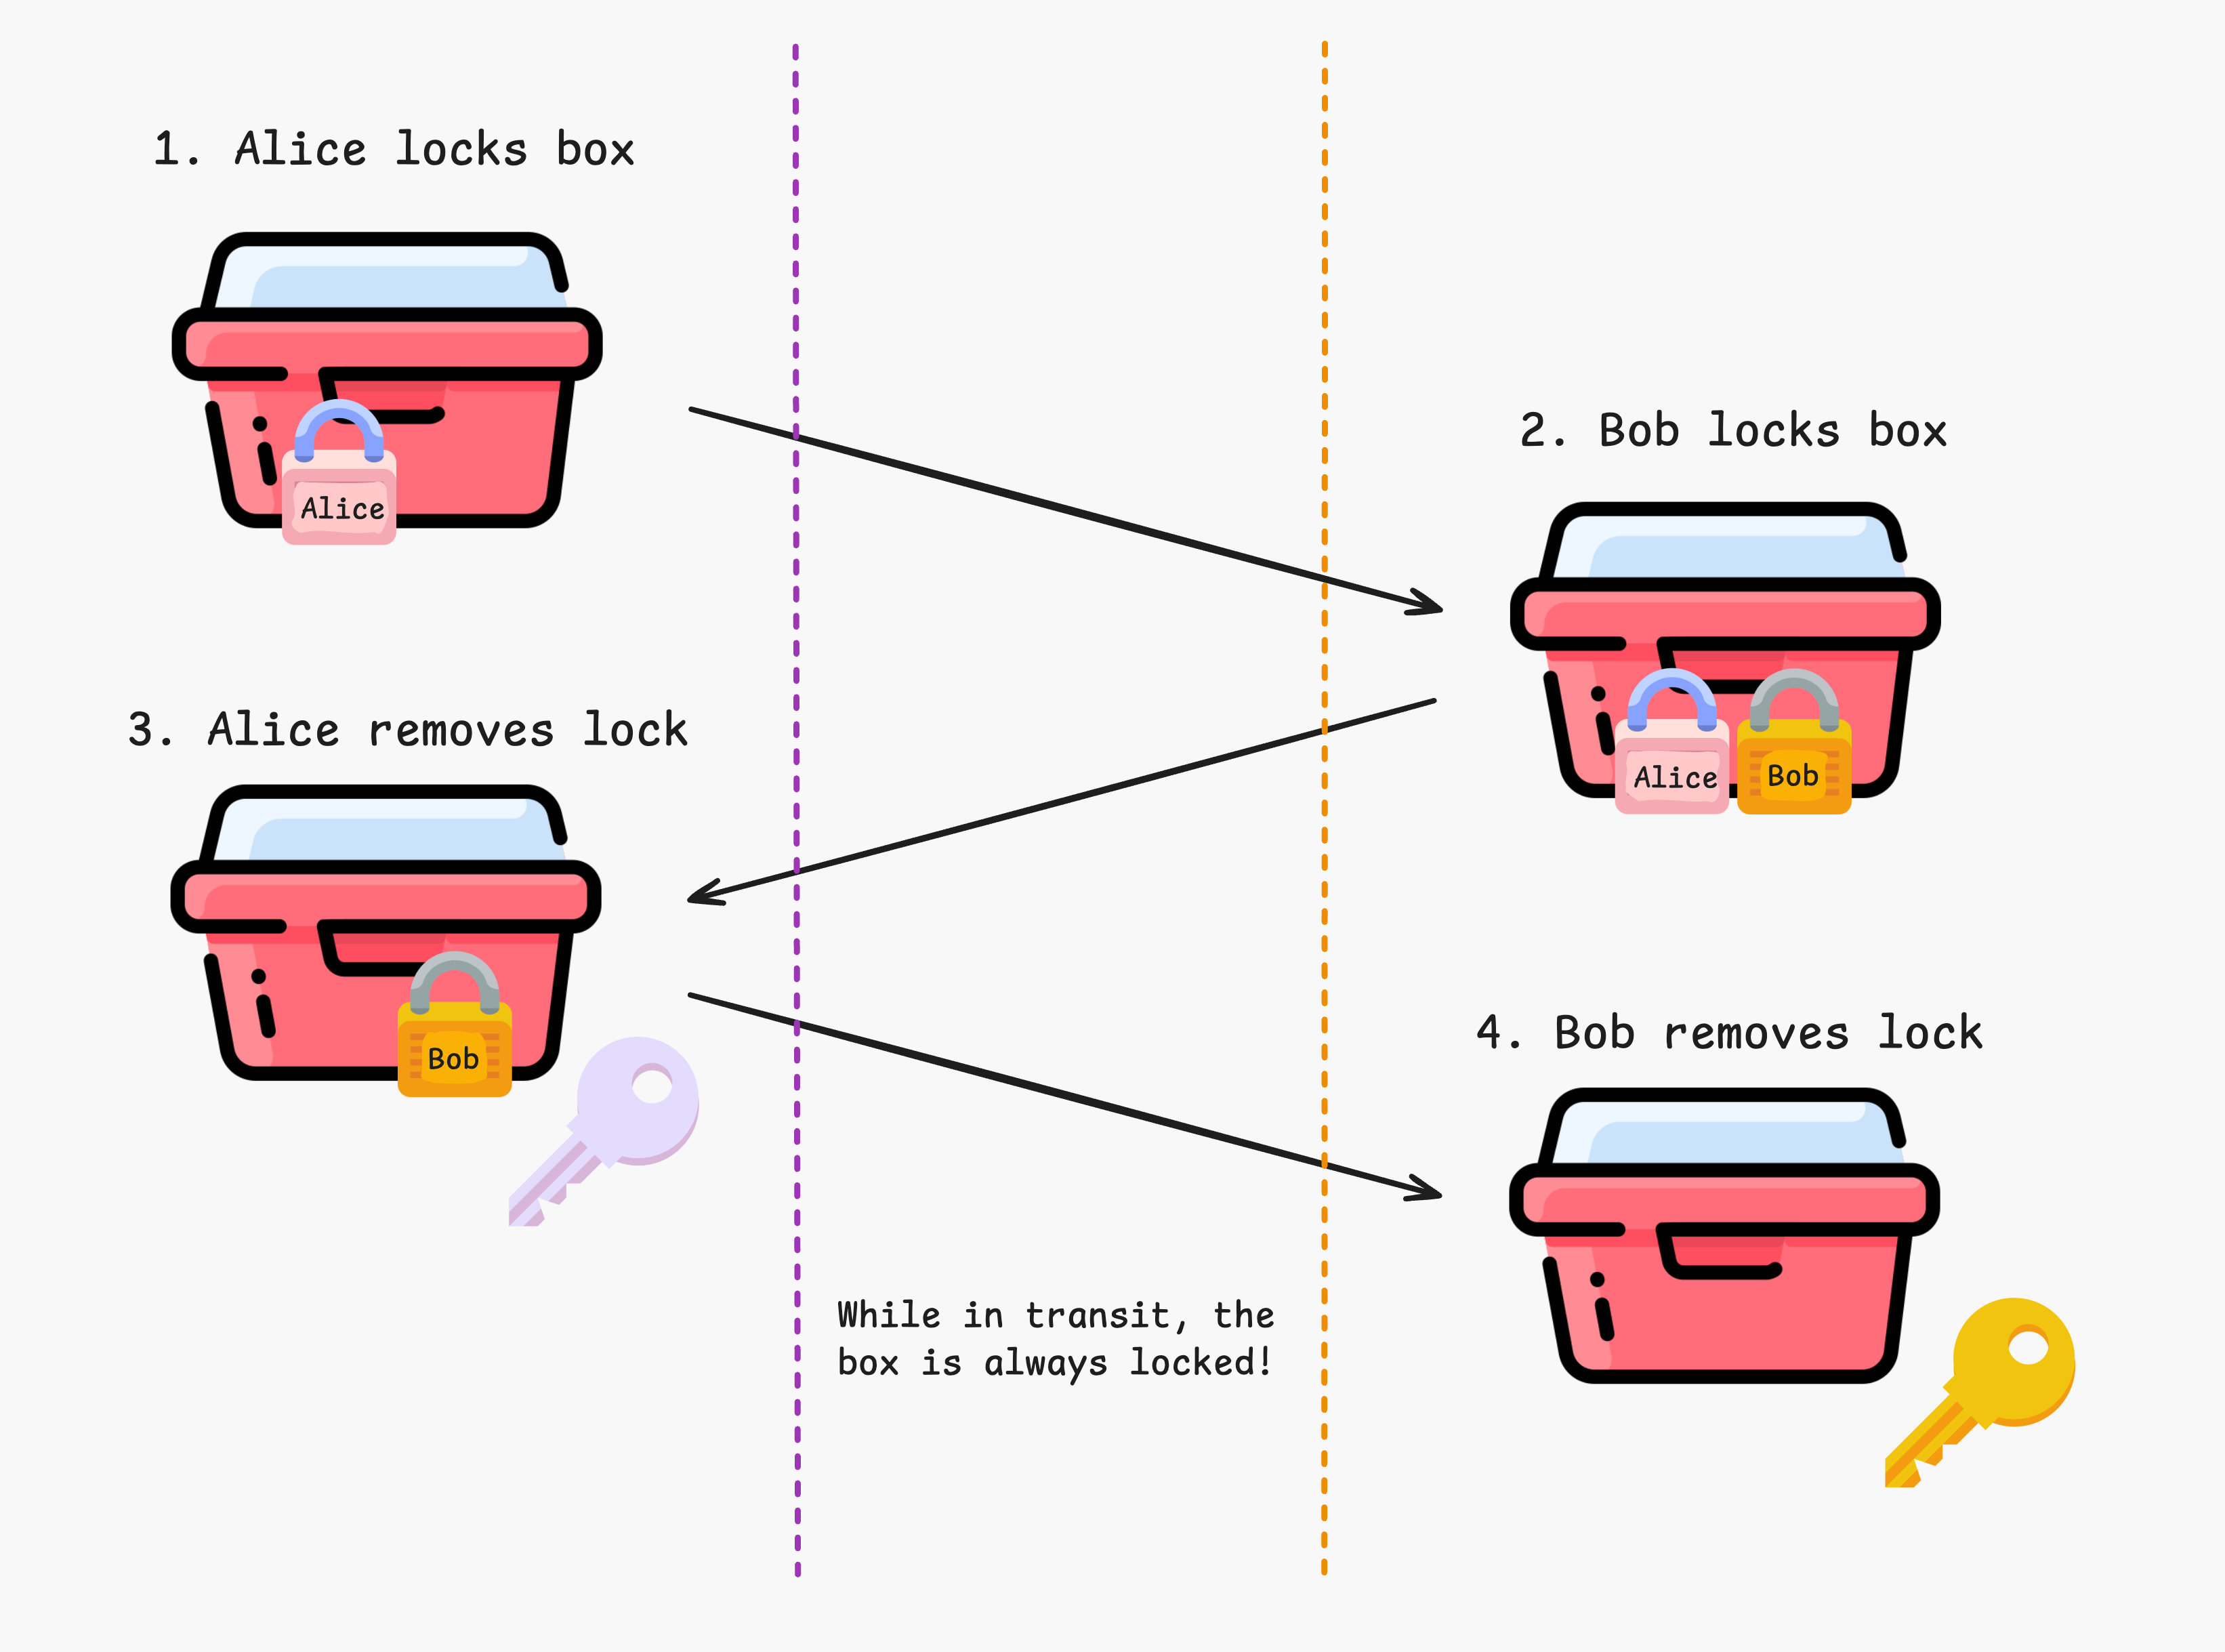
\includegraphics[width=0.9\linewidth]{figures/key-exchange-padlocks.png}
	\end{center}
\end{remark}

We now consider one of the most famous key exchange methods, which is called the \textit{Diffie-Hellmann} key exchange algorithm, and is one of the most famous methods.

Let $p$ be a large prime, and $g$ be a primitive root modulo $p$.
\begin{enumerate}
    \item Alice chooses a number $\alpha$ and sends $g^\alpha \pmod p$ to Bob.
    \item Bob chooses a number $\beta$ and sends $g^\beta \pmod p$ to Alice.
    \item Both parties now compute $k = g^{\alpha\beta} = (g^\alpha)^\beta = (g^\beta)^\alpha$, and use this as their secret key.
\end{enumerate}
Neither party knows both $\alpha$ and $\beta$, only their own, which means no attacker can steal all of the information required to compute $k$. This system therefore works even if Alice and Bob communicate only on a channel compromised by Eve!

To break this system and find $k$, Eve must compute $g^{\alpha\beta}$ using only $g$, $g^\alpha$, and $g^\beta$. It is conjectured (but not strictly proven) that this is as hard as the discrete logarithm problem.

% ================================================================== %

\subsection{Signatures and Authenticity}

We now consider another desideratum: message signatures. When Alice sends an encrypted secret message to Bob, she may have multiple goals in mind.

\begin{enumerate}
    \item Secrecy/Confidentiality: both Alice and Bob can be absolutely confident that no third party has read the original unencrypted message.
    \item Authenticity: both Alice and Bob can be absolutely confident that they are indeed talking to each other, and not a third party.
    \item Integrity: both Alice and Bob can be absolutely confident that no third party has tampered with the original message.
\end{enumerate}

Suppose Bob wants to be absolutely certain that the person with whom they are in communication is Alice rather than an impostor. How might we achieve this using RSA?

If Alice's private key is $(N, d)$ and her public key is $(N, e)$, then anyone can encrypt a message but only Alice can decrypt it. We might think to ``flip this around", and get Alice to encrypt using the \textit{private} key $(N, d)$: remember that RSA is entirely symmetrical in $d$ and $e$.

In fact, this is how the process works! Bob picks some arbitrary message $\mu$, and sends it to Alice without encrypting it. Alice then encrypts this message using $(N, d)$ as the encryption key (her private key) and sends back the result. Then, anyone can decrypt this message, but that doesn't matter, since it was arbitrary! In particular, Bob can decrypt it using $(N, e)$, and verify that the result matches the original text $\mu$.

The only way to create a message which decrypts to $\mu$ under the public key $(N, e)$ is to have the private key $d$, and so Bob knows that his interlocutor must be Alice!

We now consider the problem of \textit{integrity}. First, why is this even important?

\begin{remark}[Homomorphism Attack]
	\label{remark-homomorphism-attack}
    Suppose a bank creates a message of the form $(m_1, m_2, m_3)$, denoting the name of the client $m_1$, the amount of money $\$m_2$ to be credited to their account, and the password $m_3$ of the person authorising the transaction.
    
    These messages are encoded using RSA as $(z_1, z_2, z_3) = (m_1^e, m_2^e, m_3^e)$ all modulo $N$ using the bank's public encryption key $(N, e)$. Only the bank can decrypt this code.
    
    An attacker can enter into a transaction which credits \$100 to their account. Then, they can steal the encrypted password, or for example change $z_2$ to $z_2^3 \equiv m_2^{3e}$, stealing \$1 million!
\end{remark}

\begin{note}
	Even if an attacker didn't know that RSA was being used, they could simply transmit the same message repeatedly. We can prevent this attack vector by insisting that every message comes with a \textit{timestamp}.
\end{note}

So for integrity, we might want to consider the signature of a \textit{message}, rather than the sender. We suppose that all users have a private key and a public key. We want a \textit{signature map}:
\[
s : \calM \times \calK \to \calS
\where \begin{cases}
	\calM & \text{is the set of all possible messages} \\
	\calK & \text{is the set of all possible keys} \\
	\calS & \text{is the set of all possible signatures} \\
\end{cases}
\]
Alice signs a message $m$ with $s(m, K_A)$, where $K_A \in \calK$ is her private key. Ideally, Bob can verify that this is Alice's signature using Alice's public key $K_A'$. The signature should therefore be a \textit{trapdoor} function: something which is very easy to do one way and very difficult to reverse, much like in the discrete logarithm problem.

For example, we may use RSA. If Alice has private key $(N, d)$ and public key $(N, e)$, then she may sign a message $m$ with $s = m^d \pmod N$. Anyone can verify that $(m, s)$ is a valid signed message using the public key $(N, e)$, and therefore knows that Alice has sent the message!

\begin{definition}[Hash Function]
    A \textit{hash function} is a one-way function which is pre-image resistant and collision-resistant. In particular, $h : \calM \to \set{1, \dots, N}$ is a hash function if:
    \begin{enumerate}
	    \item Given a message $m \in \calM$, it is easy to hash the message and compute $h(m)$.
	    \item Given $1 \leq H \leq N$, it is very difficult to recover the original message $m$ with $H = h(m)$.
	    \item Given two messages $m_1 \neq m_2$ in $\calM$, the hashes $h(m_1)$ and $h(m_2)$ are different with an extremely high probability.
	\end{enumerate}
	In practice, these hash functions are constructed in such a way as to be ``very non-local", or chaotic: tiny changes to the input message $m$ (say flipping one bit of a binary string) makes the resulting hash totally different in a very unpredictable way.
	
	Hash functions are publicly known. Some of the most common ones are SHA-256 and MD5, which use a large sequence of binary operations and ``mixing up the data".
\end{definition}

\begin{corollary}
    It is easy to check that some data input maps to a given hash value. However, if the input data is unknown, it is deliberately very difficult to reconstruct.
\end{corollary}

\begin{corollary}
    A hash function is a trapdoor function!
\end{corollary}

This is a huge advantage, because it allows us to check data integrity too! When Alice wants to send a message to Bob, she encrypts her plaintext $\mu$ using Bob's public key to create an encrypted message $m$. She then computes the hash $h(m)$ using the publicly agreed hash function, then uses her own private key to encrypt $h(m)$ to form the signature. She then sends $m$ and $s$. Bob can:
\begin{enumerate}
    \item Decrypt $m$ using his own private key, and thus both parties are confident that only Bob is able to read the original message $\mu$.
    \item Compute $h(m)$ himself using the publicly agreed hash function.
    \item Decrypt the signature using Alice's public key. This should result in the hash $h(m)$ which he calculated. If there is a discrepancy, then he knows that either some message was corrupted, or that he is not talking to Alice. But if there is a match, then he knows for sure that only Alice could possibly have sent this message!
\end{enumerate}

We therefore have a ``perfect" system! Alice has total confidence that only Bob can see the message, and Bob has total confidence that Alice sent the exact message $\mu$ he decrypted.

An attacker Eve can read $m$ and $s$, and can decrypt $s$ into $h(m)$ using Alice's public key. She can therefore also verify that the message came from Alice, but not read it. What if Eve wants to forge a message from Alice? She could easily find $h(m)$, but would need to sign it using Alice's private key, which is difficult.

Even if Alice finds a way to alter the message in transit (such as in the Homomorphism Attack from Remark \ref{remark-homomorphism-attack}), any slightly changed version $m'$ of $m$ changes $h(m')$ to something completely unrecognisable, and so Eve could not sign the new hash with Alice's private key.

Another common signature scheme is the ElGamal Signature Scheme, developed in 1985. As usual, we take $p$ to be a large prime and $g$ to be a primitive root modulo $p$. Furthermore, we take the function $h : \calM \to \set{1, \dots, p-1}$ to be a collision-resistant hash function.

Alice first chooses a random integer $1 < u < p$ to be her private key, and then sets the public key to be $(p, g, y)$, where $y \equiv g^u \pmod p$. This is published for anyone to see.

When Alice wants to sign a message $m$, she chooses a random key $1 < k < p$ which is coprime to $p-1$, and finds $k'$ with $kk' = 1 \pmod{p-1}$. She then calculates the two numbers:
\[
r \equiv g^k \pmod p
\qquad
s \equiv k'(h(m) - ur) \pmod{p-1}.
\]
This $s$ has the property that $h(m) \equiv ur + ks \pmod{p-1}$. She then sends the signature $(r, s)$ for the message $m$. In order to verify that Alice sent the original message, anyone can compute $v_1 = y^r \cdot r^s$ and $v_2 = g^{h(m)}$, both modulo $p$.

\begin{proposition}[ElGamal Check]
    The signature $(r, s)$ is valid for message $m$ if $v_1 = v_2$.
\end{proposition}

\begin{prf}
    We have $v_1 \equiv y^r \cdot r^s \equiv (g^u)^r \cdot (g^k)^s \equiv g^{ur} \cdot g^{ks} \equiv g^{ur + ks} \equiv g^{h(m)} \equiv v_2 \pmod p$ if $v_1$ and $v_2$ are constructed correctly using the above signature scheme, where the crucial equivalence follows from the relation $h(m) \equiv ur + ks \pmod{p-1}$.
    
    It is harder to show that this signature is difficult to forge. Given some $m$, there is no other $m$ with the same $v_2 = g^{h(m)}$, so the attacker can only choose $r$ and $s$. But this only works out to the correct $v_1$ if $r$ and $s$ match the correct values, which can only be calculated knowing $u$.
\end{prf}

\begin{note}
	Of course, like any signature scheme, this is vulnerable to \textit{replay attacks}, where an attacker simply repeats a message they've already seen transmitted with the corresponding signature! To combat this attack, we can insist that each message comes with a ``nonce" (number used once, like a timestamp), which allows the recipient to ensure each message only comes through one time.
\end{note}

\end{document}
